% !TEX program = xelatex
% 原图版项目：主文件与原图目录须一同保存。
\documentclass[UTF8,zihao=-4,fontset=fandol,a4paper]{ctexart}
\usepackage[margin=24mm,headheight=16pt,headsep=8mm,footskip=12mm]{geometry}
\usepackage{amsmath,amssymb,bm,mathtools}
\usepackage{xcolor,graphicx,tikz,booktabs,array,tabularx,longtable}
\usepackage{enumitem,fancyhdr,caption,hyperref}
\definecolor{ink}{HTML}{233E50}
\definecolor{soft}{HTML}{F0F4F6}
\definecolor{muted}{HTML}{586774}
\hypersetup{hypertexnames=false,colorlinks=true,linkcolor=ink,urlcolor=ink,pdftitle={理论力学讲义：第二章 质点组力学（修订完善版）},pdfauthor={}}
\ctexset{section={format=\Large\bfseries\color{ink}},subsection={format=\large\bfseries},subsubsection={format=\normalsize\bfseries}}
\renewcommand{\thesection}{2.\arabic{section}}
\renewcommand{\theequation}{2.\arabic{equation}}
\renewcommand{\thefigure}{2.\arabic{figure}}
\setcounter{tocdepth}{2}
\linespread{1.18}
\setlength{\parskip}{3pt}
\setlength{\emergencystretch}{2em}
\clubpenalty=10000 \widowpenalty=10000
\setlist{nosep,topsep=5pt,leftmargin=2em}
\setlength{\textfloatsep}{13pt}
\setlength{\intextsep}{12pt}
\captionsetup{font=small,labelfont=bf,skip=6pt,hypcap=false}
\pagestyle{fancy}
\fancyhf{}
\fancyhead[L]{\small\color{muted}理论力学讲义}
\fancyhead[R]{\small\color{muted}第二章\quad 质点组力学}
\fancyfoot[C]{\small\thepage}
\renewcommand{\headrulewidth}{0pt}
\newcommand{\vect}[1]{\bm{#1}}
\newcommand{\dd}{\mathrm d}
\newcommand{\er}{\vect e_r}
\newcommand{\et}{\vect e_\theta}
\newcommand{\vt}{\vect e_t}
\newcommand{\vn}{\vect e_n}
\newcommand{\important}[1]{\par #1\par}
\newcounter{example}
\newcommand{\example}[1]{\Needspace{5\baselineskip}\refstepcounter{example}\subsubsection*{例\theexample\quad #1}}
\newcommand{\solution}{\setcounter{solutionstep}{0}\par\nopagebreak[4]\smallskip\nopagebreak[4]\noindent\textbf{解答}\quad}


\newcommand{\Mtot}{M}
\newcommand{\CM}{\mathrm C}
\newcounter{exercise}
\newcommand{\exercise}[1]{\Needspace{5\baselineskip}\refstepcounter{exercise}\subsubsection*{训练题\theexercise\quad #1}}

\makeatletter
\newcommand{\Needspace}[1]{\par\if@nobreak\else\penalty0\begingroup\dimen0=#1\relax\dimen2=\pagegoal\advance\dimen2 by-\pagetotal\ifdim\dimen0>\dimen2\newpage\fi\endgroup\fi}
\makeatother
\let\SavedSection\section
\renewcommand{\section}{\Needspace{8\baselineskip}\SavedSection}
\let\SavedSubsection\subsection
\renewcommand{\subsection}{\Needspace{6\baselineskip}\SavedSubsection}
\newcommand{\OriginalFigure}[2]{%
\par\begin{center}\begin{minipage}{\linewidth}\centering
\includegraphics[width=.91\linewidth,height=6.2cm,keepaspectratio]{原图/#1}%
\captionof{figure}{#2}\label{fig:orig-#1}\end{minipage}\end{center}\par}
\newcommand{\OriginalPanel}[1]{\includegraphics[width=.46\linewidth,height=4.6cm,keepaspectratio]{原图/#1}}


\usetikzlibrary{arrows.meta,calc,positioning,angles,quotes,patterns,decorations.pathmorphing}
\tikzset{every picture/.style={>=Stealth},every node/.style={font=\small},force/.style={->,thick,ink},guide/.style={dashed,muted}}
\newsavebox{\LessonFigureBox}
\newcommand{\TeachingFigure}[2]{%
\par\begin{center}\begin{minipage}{\linewidth}\centering
\sbox{\LessonFigureBox}{\input{补充图/#1.tex}}%
\ifdim\wd\LessonFigureBox>.98\linewidth
\resizebox{.98\linewidth}{!}{\usebox{\LessonFigureBox}}%
\else\usebox{\LessonFigureBox}\fi
\captionsetup{hypcap=false}\captionof{figure}{#2}\label{fig:lesson-#1}
\end{minipage}\end{center}\par}

\newsavebox{\QuestionDrawing}
\newcommand{\QuestionStatement}[3]{%
\par\noindent\begin{minipage}{\linewidth}%
\begin{minipage}[t]{.63\linewidth}\vspace{0pt}\raggedright\setlength{\parindent}{0pt}#1\end{minipage}\hfill%
\begin{minipage}[t]{.34\linewidth}\vspace{2pt}\centering%
\sbox{\QuestionDrawing}{\input{题图/#2.tex}}%
\resizebox{.98\linewidth}{!}{\usebox{\QuestionDrawing}}\par\vspace{3pt}{\small #3}%
\end{minipage}\end{minipage}\par\smallskip}
\newcommand{\LongQuestionStatement}[3]{\par #1\par\smallskip\noindent\begin{minipage}{\linewidth}\centering\sbox{\QuestionDrawing}{\input{题图/#2.tex}}\resizebox{.42\linewidth}{!}{\usebox{\QuestionDrawing}}\par{\small #3}\end{minipage}\par\smallskip}
\newcounter{solutionstep}
\newcommand{\Step}[1]{\ifnum\value{solutionstep}>0\par\smallskip\noindent\fi\stepcounter{solutionstep}\textbf{（\arabic{solutionstep}）#1}\quad}


\newsavebox{\SolutionDrawing}
\newsavebox{\SolutionScaled}
\newcommand{\SolutionFigure}[2]{%
\par\addvspace{6pt}\noindent\begin{minipage}{\linewidth}\centering%
\sbox{\SolutionDrawing}{\input{解答图/#1.tex}}%
\sbox{\SolutionScaled}{\resizebox{.88\linewidth}{!}{\usebox{\SolutionDrawing}}}%
\ifdim\ht\SolutionScaled>5.6cm\resizebox{!}{5.6cm}{\usebox{\SolutionDrawing}}\else\usebox{\SolutionScaled}\fi%
\captionof{figure}{#2}\label{fig:solution-#1}\end{minipage}\par\addvspace{6pt}}


\begin{document}

\begin{titlepage}
\vspace*{15mm}
\noindent{\Large\color{muted}理论力学\quad 课程讲义}
\vspace{16mm}
\par\noindent{\Huge\bfseries 第二章}
\vspace{5mm}
\par\noindent{\Huge\bfseries\color{ink}质点组力学}
\vspace{11mm}
\par\noindent{\large 整体运动、相对运动与相互作用}
\vspace{17mm}
\begin{center}
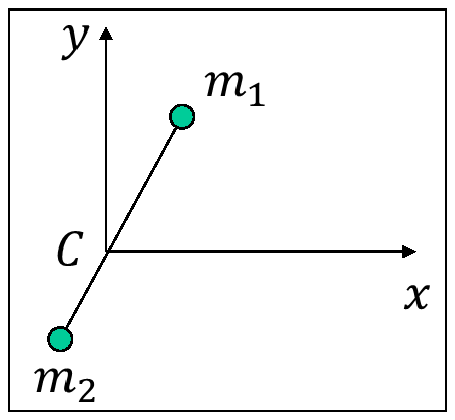
\includegraphics[width=.8\linewidth,height=6.5cm,keepaspectratio]{原图/two_body_cm}
\end{center}
\vfill
\noindent\begin{minipage}{\linewidth}\small
从质心出发，把质点组的整体运动与内部运动联系起来。依次讨论动量、角动量和能量定理，再用两体问题、碰撞与散射、变质量运动和位力定理说明这些方法的应用。正文包含推导、完整例题和训练题解答，配图说明模型、推导和结果之间的联系。\par\medskip
2026 年 10 月
\end{minipage}
\end{titlepage}

\pagenumbering{roman}
\section*{符号与基本约定}
本章研究由多个质点构成的系统。核心问题有两个：整个系统怎样运动，以及系统内部怎样发生相对运动。质心把这两类运动联系起来；动量、角动量和能量则分别揭示不同的动力学约束。

所有坐标方向、角度起算方向和速度所对应的参考系均在题干或解答中说明。课件原图沿用原有标注；图题说明其与正文的符号对应。定量图注明所取参数和适用范围。图中曲线和物体大小用于说明几何关系；未标明数值比例时，不作为测量依据。

本章默认使用经典力学。除变质量部分外，质点的质量均为常数；除另有说明外，参考系为惯性系，绳和杆为无质量理想连接件。位力定理的量子形式单独说明其平均与边界条件。
\textbf{统一记号}\quad
$M=\sum_i m_i$；$\vect R$ 为质心位置，$\vect V=\dot{\vect R}$；
$\vect r'_i=\vect r_i-\vect R$，$\vect v'_i=\vect v_i-\vect V$。
两体问题取 $\vect r=\vect r_1-\vect r_2$，$\mu=m_1m_2/M$。
$\vect F_{ij}$ 表示质点 $j$ 对质点 $i$ 的力。
\clearpage
\begingroup\small\linespread{1.05}\selectfont
\makeatletter
\renewcommand\@pnumwidth{2.5em}\renewcommand*\l@section[2]{\addvspace{4pt}\@dottedtocline{1}{0em}{2.7em}{\bfseries #1}{\bfseries #2}}
\renewcommand*\l@subsection{\@dottedtocline{2}{1.5em}{3.2em}}
\makeatother
\tableofcontents\endgroup\clearpage
\pagenumbering{arabic}
\section{质点组的运动学与质心}\label{sec:c2-1}
\subsection{系统边界、内力与外力}\label{sub:c2-1.1}
质点组是由若干质点组成的系统，质点之间的距离可以变化。刚体是其中质点间距离保持不变的特殊模型；液体、气体、行星系统、由绳或弹簧连接的物体，均可作为质点组研究。这里的“内部距离可变”与“系统总质量随时间变化”是两件不同的事。

选定系统以后，来自系统外部物体的力为外力，成员之间的相互作用力为内力。同一根绳的拉力是否为内力，取决于绳以及绳两端物体是否都包含在系统中。例如，把两个悬挂重物作为系统，地球引力和支架作用均为外力；只取其中一个重物，则绳的拉力也是外力。

对第 $i$ 个质点，
\begin{equation}
m_i\ddot{\vect r}_i=\vect F_i^{\rm ext}+\sum_{j\ne i}\vect F_{ij}.
\end{equation}
若相互作用满足 $\vect F_{ij}=-\vect F_{ji}$，按每一对质点只计一次，有
\begin{equation}
\sum_i\vect F_i^{\rm int}
=\sum_{i<j}(\vect F_{ij}+\vect F_{ji})=0.
\end{equation}
这并不意味着内力不起作用。内力能改变各成员的动量、相对位置、内部动能以及形变能。

关于固定点 $O$，一对内力的合力矩为
\begin{equation}
\vect r_i\times\vect F_{ij}+\vect r_j\times\vect F_{ji}
=(\vect r_i-\vect r_j)\times\vect F_{ij}.
\end{equation}
只有进一步要求内力沿两质点连线，即中心力形式，才能保证这一力矩为零。大小相等、方向相反本身不足以保证内力矩抵消。
\OriginalFigure{internal_central_pair}{两质点的中心内力沿连线、等大反向；关于 $O$ 的内力合力矩为零。 原图 $f_{ij}$ 对应正文的 $\mathbf F_{ij}$。}
\subsection{离散系统与连续物体的质心}\label{sub:c2-1.2}
定义质心
\begin{equation}\label{eq:CM}
\vect R=\frac1M\sum_i m_i\vect r_i,\qquad M=\sum_i m_i.
\end{equation}
其分量分别为 $X=\sum_i m_ix_i/M$、$Y=\sum_i m_iy_i/M$、
$Z=\sum_i m_iz_i/M$。质量恒定时，求导得
\begin{equation}
\vect P=\sum_i m_i\vect v_i=M\vect V,\qquad
\sum_i m_i\vect r'_i=0,\quad \sum_i m_i\vect v'_i=0.
\end{equation}
质心是位置的质量加权平均，不必落在物体内部。
\OriginalFigure{center_of_mass_coordinates}{质心 $C$ 与第 $i$ 个质点的位置关系。原图 $\mathbf r_C$ 对应正文的 $\mathbf R$，$x_C,y_C,z_C$ 对应 $X,Y,Z$。}均匀圆环的质心在圆心，均匀弯曲细杆的质心也可能位于杆外。

连续物体用积分代替求和：
\begin{equation}
\vect R=\frac{\int\vect r\,\dd m}{\int\dd m},\qquad
\dd m=
\begin{cases}
\lambda\,\dd s,&\text{细线},\\
\sigma\,\dd A,&\text{薄片},\\
\rho\,\dd V,&\text{体积}.
\end{cases}
\end{equation}
均匀物体的常数密度约去后，可直接求线、面积或体积的几何形心。对称性可先确定若干分量：若关于 $yz$ 平面对称，则 $X=0$；但轴向分量一般仍须积分。

改变坐标原点 $\vect r_i\mapsto\vect r_i-\vect a$ 时，质心也改变为
$\vect R-\vect a$，而 $\vect r'_i$ 不变。因此质心的定义与原点选择相容。

\example{三角形薄片与三个顶点质点}
\label{ex:c2-1}
\QuestionStatement{均匀三角形薄片顶点为 $\vect a,\vect b,\vect c$，求质心，并与三个等质量顶点质点比较。
以 $G$ 表示质心、$D$ 表示 $BC$ 中点，说明中线上的分割比；积分中须给出质量或面积权重。}{ex01}{例1题图}
% BEGIN DETAILED ANSWER ex01
\solution \Step{明确系统、坐标与约束} 三角形内的面密度为常数 $\sigma$，因此质心是面积加权平均。取 $A,B,C$ 三个顶点对应位置 $\vect a,\vect b,\vect c$，用两个无量纲参数表示内部点；不能仅以图形外观把薄片当成三个质点，须先证明两种平均相同。

图~\ref{fig:solution-ex01}~中顶点 $A,B,C$ 与中线交点 $G$，给出了本题列式所用的方向、位置或分区关系；图右侧列出由这些条件得到的关键方程及下一步计算。
\SolutionFigure{ex01}{例1的分析与计算}

\Step{列出方程并求解} 用重心坐标
$\vect r=\vect a+u(\vect b-\vect a)+v(\vect c-\vect a)$，
$u\ge0,v\ge0,u+v\le1$。面积元中的常数雅可比在分子、分母中约去。
积分域面积为 $1/2$，而
\[
\int_0^1\!\int_0^{1-u}u\,\dd v\,\dd u=\frac16,\qquad
\int_0^1\!\int_0^{1-u}v\,\dd v\,\dd u=\frac16.
\]
故 $\bar u=\bar v=1/3$，
\begin{equation}
\vect R=\frac{\vect a+\vect b+\vect c}{3}.
\end{equation}
三个等质量顶点质点给出完全相同的质心。若 $D=(\vect b+\vect c)/2$，
则 $\vect R=\vect a+\frac23(\vect D-\vect a)$，质心将每条中线按 $2:1$ 分割。

\Step{补出重心坐标积分的归一化}
设雅可比常数为 $J_0=|(\vect b-\vect a)\times(\vect c-\vect a)|$，则
\[
M=\sigma J_0\int_0^1\int_0^{1-u}\dd v\dd u=\sigma J_0/2,
\quad \int u\dd m=\sigma J_0/6.
\]
故 $\langle u\rangle=(\sigma J_0/6)/(\sigma J_0/2)=1/3$，$v$ 同理，第三个重心坐标 $1-u-v$ 的平均也为 $1/3$。
三个等质量顶点的平均是离散求和，本题薄片是连续积分；相同结果来自均匀性和三角形的仿射结构。沿中线 $AG$ 有 $AG=2AD/3$，所以 $AG:GD=2:1$。若顶点质量不相等或面密度不均匀，不能沿用这一比例。

% END DETAILED ANSWER ex01
\TeachingFigure{c2-diagram-02}{三角形质心位于三条中线的交点}


\subsection{组合体、挖孔与负质量法}\label{sub:c2-1.3}
把物体分解为若干已知质心的部分，整体质心为
\[
\vect R=\frac{\sum_k M_k\vect R_k}{\sum_kM_k}.
\]
挖去的部分可赋予负质量：这只是积分差的记账方法，不表示存在物理上的负质量。

\example{圆盘挖去两个相同圆孔}
\label{ex:c2-2}
\QuestionStatement{半径为 $R$ 的均匀圆盘挖去两个半径为 $r$ 的孔。两孔中心到圆盘中心的距离均为 $R/2$，夹角为 $60^\circ$，关于竖直轴对称且位于上半盘。设孔不重叠，求剩余薄片质心。
同时写出保证两个完整圆孔位于盘内且互不重叠的半径范围。}{ex02}{例2题图}
% BEGIN DETAILED ANSWER ex02
\solution \Step{明确系统、坐标与约束} 把被挖掉的两个完整圆孔视为从原圆盘的质量积分中减去两项。设剩余质量为 $M_{\rm rem}$，面密度相同，则面积比就是质量比，密度将在求质心时约去。左右对称先给出 $X=0$，只需计算竖直一阶矩。

图~\ref{fig:solution-ex02}~中位于 $y=\sqrt3R/4$ 的两个负质量圆孔，给出了本题列式所用的方向、位置或分区关系；图右侧列出由这些条件得到的关键方程及下一步计算。
\SolutionFigure{ex02}{例2的分析与计算}

\Step{列出方程并求解} 以圆盘中心为原点，$y$ 向上。孔中心
\[
(x_1,y_1)=\left(-\frac R4,\frac{\sqrt3R}4\right),\qquad
(x_2,y_2)=\left(\frac R4,\frac{\sqrt3R}4\right).
\]
原盘质量 $M_0=\sigma\pi R^2$，每孔质量 $m=\sigma\pi r^2$。于是
\begin{equation}
X=0,\qquad
Y=\frac{-m(y_1+y_2)}{M_0-2m}
=-\frac{\sqrt3Rr^2}{2(R^2-2r^2)}.
\end{equation}
孔在上方，剩余薄片的质心必向下偏移，负号可由这一几何检查判定。两孔中心距为 $R/2$，故不重叠要求 $r\le R/4$，此时孔也包含在原盘内。

\Step{展开负质量法的两条独立收支}
原盘的一阶矩为零，故
\[
M_{\rm rem}=\sigma\pi(R^2-2r^2),\qquad
M_{\rm rem}Y=0-\sigma\pi r^2\frac{\sqrt3R}{4}
-\sigma\pi r^2\frac{\sqrt3R}{4}.
\]
相除得到前式。此处不是对两个孔中心直接取平均，而是对剩余薄片作质量加权。
两孔中心距为 $R/2$，不重叠需 $2r\le R/2$；每孔距盘心 $R/2$，包含条件为 $R/2+r\le R$。合并得 $0<r\le R/4$，同时保证剩余质量严格为正。
$r\to0$ 时 $Y\to0$；在允许的最大 $r=R/4$ 时 $Y=-\sqrt3R/28$，仍在圆盘内且偏向下方，验证符号及数量级。

% END DETAILED ANSWER ex02
\OriginalFigure{disk_two_holes}{原圆盘上部挖去两相同圆孔；剩余部分的质心向下偏移。}

\subsection{连续体质心的积分实例}\label{sub:c2-1.4}
\example{均匀实心半球与厚半球壳}
\label{ex:c2-3}
\QuestionStatement{求半径为 $a$ 的均匀实心半球的质心；再求内半径为 $a$、外半径为 $b$ 的均匀厚半球壳质心。
取赤道面为 $z=0$、对称轴向上，$0\le a<b$；检验实心极限与薄壳极限。}{ex03}{例3题图}
% BEGIN DETAILED ANSWER ex03
\solution \Step{明确系统、坐标与约束} 以球心为原点，半球对 $x=0,y=0$ 两平面对称，故 $X=Y=0$。水平薄层内密度恒定，取 $\dd m=\rho A(z)\dd z$；对厚壳则把外半球和内半球的体积分分别相减，不能直接对两个半径作算术平均。

图~\ref{fig:solution-ex03}~中半球的水平截面和厚壳内外半径，给出了本题列式所用的方向、位置或分区关系；图右侧列出由这些条件得到的关键方程及下一步计算。
\SolutionFigure{ex03}{例3的分析与计算}

\Step{列出方程并求解} 以赤道平面为 $z=0$，半球位于 $z\ge0$。实心半球横截面积
$A(z)=\pi(a^2-z^2)$，所以
\[
V=\int_0^aA(z)\dd z=\frac{2\pi a^3}{3},\qquad
\int z\dd V=\int_0^a\pi z(a^2-z^2)\dd z=\frac{\pi a^4}{4}.
\]
因此 $X=Y=0$，$Z=3a/8$。

另用球坐标 $z=s\cos\theta$，$\dd V=s^2\sin\theta\,\dd s\,\dd\theta\,\dd\phi$，
$0\le\theta\le\pi/2$，可得
\[
\int z\dd V=
\int_0^{2\pi}\!\dd\phi\int_0^{\pi/2}\!\cos\theta\sin\theta\,\dd\theta
\int_0^a s^3\dd s=\frac{\pi a^4}{4}.
\]
厚半球壳由两实心半球相减：
\begin{equation}
Z=\frac{3(b^4-a^4)}{8(b^3-a^3)}.
\end{equation}
$a=0$ 时恢复实心结果 $3b/8$；薄壳极限 $b\to a$ 给出 $Z=a/2$。
实心半球与薄半球壳的质心不同，不能混用。

\Step{把壳层的一阶矩和质量分别相减}
外、内半球的质量分别为 $2\pi\rho b^3/3,2\pi\rho a^3/3$，一阶矩分别为 $\pi\rho b^4/4,\pi\rho a^4/4$，因此
\[
Z=\frac{\pi\rho(b^4-a^4)/4}{2\pi\rho(b^3-a^3)/3}.
\]
在 $b\to a$ 时分子、分母同时趋零，不能分别代零；因式分解或求导可得
$\lim Z=(3/8)(4a^3)/(3a^2)=a/2$。
实心半球的质量更多分布在赤道附近，质心较低；薄半球壳质量集中于曲面，得到更高的 $a/2$。这也解释了两类物体不能只因外轮廓相同而使用同一个质心公式。

% END DETAILED ANSWER ex03
\TeachingFigure{c2-diagram-04}{实心半球的水平切片与厚半球壳的体积差；右图 $a$、$b$ 分别为内外半径}
\OriginalFigure{hemisphere}{均匀实心半球及其坐标轴，半径为 $a$。}

\example{圆锥及其沿轴剖开的半圆锥}
\label{ex:c2-4}
\QuestionStatement{均匀圆锥底面半径为 $a$，高为 $h$。求完整圆锥的质心，以及沿包含轴的平面剖开、保留 $x\ge0$ 部分后的质心。
以底面中心为原点、轴向上为 $z$，补齐半圆截面的一阶矩积分。}{ex04}{例4题图}
% BEGIN DETAILED ANSWER ex04
\solution \Step{明确系统、坐标与约束} 完整圆锥绕对称轴旋转不改变质量分布，所以质心位于该轴。半圆锥仅保留 $x\ge0$ 后，仍关于 $y=0$ 对称，$Y=0$；每个水平截面的面积恰为整圆的一半，因此轴向平均高度不变，横向坐标须另外积分。

图~\ref{fig:solution-ex04}~中$x\ge0$ 半圆截面的形心及顶点高度，给出了本题列式所用的方向、位置或分区关系；图右侧列出由这些条件得到的关键方程及下一步计算。
\SolutionFigure{ex04}{例4的分析与计算}

\Step{列出方程并求解} 先以顶点为原点、沿轴向下取 $s$。截面半径 $as/h$，截面积
$\pi a^2s^2/h^2$。故
\[
\bar s=\frac{\int_0^h s^3\dd s}{\int_0^h s^2\dd s}=\frac{3h}{4}.
\]
以底面为 $z=0$、向上为正，则 $Z=h/4$。

半圆锥仍有 $Z=h/4$，$Y=0$。高度 $z$ 处截面为半径
$r=a(1-z/h)$ 的半圆盘，其面积为 $\pi r^2/2$，面积对 $yz$ 平面的矩为
\[
\int_{x\ge0}x\,\dd A
=\int_{-\pi/2}^{\pi/2}\!\cos\phi\,\dd\phi\int_0^r s^2\dd s
=\frac{2r^3}{3}.
\]
积分得半圆锥体积 $V=\pi a^2h/6$，一阶矩为
$\int_0^h(2/3)a^3(1-z/h)^3\dd z=a^3h/6$。所以
\begin{equation}
(X,Y,Z)=\left(\frac a\pi,0,\frac h4\right).
\end{equation}

\Step{说明半圆截面的一阶矩如何进入三维平均}
半径 $r$ 的半圆盘面积为 $A_h=\pi r^2/2$，其形心横坐标为
\[
\bar x_h=\frac{2r^3/3}{\pi r^2/2}=\frac{4r}{3\pi}.
\]
高度 $z$ 对应 $r(z)=a(1-z/h)$，所以整块半圆锥
\[
X=\frac{\int_0^h\bar x_h(z)A_h(z)\dd z}{\int_0^h A_h(z)\dd z}
=\frac{(2/3)\int_0^h r(z)^3\dd z}{(\pi/2)\int_0^h r(z)^2\dd z}=a/\pi.
\]
截面形心不能不加权地沿高度平均，因为截面质量随 $r^2$ 变化。轴向坐标 $h/4$ 从底面量起，与从顶点量起的 $3h/4$ 相加为 $h$。所有结果均落在保留的半圆锥内部，$X>0$ 与去掉负半空间一致。

% END DETAILED ANSWER ex04
\TeachingFigure{c2-diagram-05}{半圆锥的水平截面为半圆盘：先求截面形心 $4r/(3\pi)$，再沿高度作体积加权}
\OriginalFigure{cone}{均匀圆锥及柱坐标示意。原图 $z$ 从顶点向下，等于正文的轴向变量 $s$；以底面向上计的高度为 $h-z$。}

\example{抛物线围成的均匀薄片}
\label{ex:c2-5}
\QuestionStatement{均匀薄片由 $y=kx^2$ 与 $y=a$ 围成，其中 $k,a>0$。求质心。
写出积分域及面积元，分别计算面积与一阶矩，并检验质心是否在薄片内部。}{ex05}{例5题图}
% BEGIN DETAILED ANSWER ex05
\solution \Step{明确系统、坐标与约束} 交点由 $kx^2=a$ 给出，故 $x\in[-b,b]$，$b=\sqrt{a/k}$；每个竖直条带从 $y=kx^2$ 延伸到 $a$。条带面积为 $(a-kx^2)\dd x$，条带的一阶矩应积分 $y\dd y\dd x$，不是只用顶边高度乘面积。

图~\ref{fig:solution-ex05}~中两条竖直边界间宽为 $\dd x$ 的面积条，给出了本题列式所用的方向、位置或分区关系；图右侧列出由这些条件得到的关键方程及下一步计算。
\SolutionFigure{ex05}{例5的分析与计算}

\Step{列出方程并求解} 关于 $y$ 轴对称，故 $X=0$。令 $b=\sqrt{a/k}$，
\[
A=\int_{-b}^b(a-kx^2)\dd x=\frac43ab,
\]
\[
\int y\,\dd A=\frac12\int_{-b}^b(a^2-k^2x^4)\dd x
=\frac45a^2b.
\]
于是 $Y=3a/5$。取适当坐标单位使 $k=1$，即得到 $y=x^2$ 的特例。

\Step{逐项算出面积与条带力矩}
\[
A=2\left[ax-\frac{kx^3}{3}\right]_0^b
=2ab(1-1/3)=4ab/3,
\]
\[
M_y=2\int_0^b\frac{a^2-k^2x^4}{2}\dd x
=a^2b-\frac{k^2b^5}{5}=4a^2b/5.
\]
使用 $kb^2=a$ 约去曲率参数，得 $Y=M_y/A=3a/5$。
也可改用水平条带：$x$ 的宽度为 $2\sqrt{y/k}$，于是
$Y=\int_0^ay\sqrt y\dd y/\int_0^a\sqrt y\dd y=3a/5$，构成独立核验。
$k$ 决定横向伸缩，关于 $y$ 的归一化分布不变，因此 $Y/a$ 不依赖 $k$，且 $0<Y<a$。

% END DETAILED ANSWER ex05
\TeachingFigure{c2-diagram-06}{抛物线薄片关于竖直轴对称，质心高度为 $3a/5$}


\example{由坐标平面截出的四面体}
\label{ex:c2-6}
\QuestionStatement{均匀四面体由 $x=0,y=0,z=0$ 和 $4x+2y+z=8$ 围成，求质心。
坐标均用同一长度单位。写出三重积分上下限和质量密度如何约去。}{ex06}{例6题图}
% BEGIN DETAILED ANSWER ex06
\solution \Step{明确系统、坐标与约束} 第一卦限中的截平面与各坐标轴交于 $2,4,8$，因此体积分最直接的次序为先 $z$、再 $y$、最后 $x$：$0\le x\le2$，$0\le y\le4-2x$，$0\le z\le8-4x-2y$。均匀密度只作为常因子，不会改变归一化质心。

图~\ref{fig:solution-ex06}~中三条截距为 $2,4,8$ 的坐标棱，给出了本题列式所用的方向、位置或分区关系；图右侧列出由这些条件得到的关键方程及下一步计算。
\SolutionFigure{ex06}{例6的分析与计算}

\Step{列出方程并求解} 截距为 $a=2,b=4,c=8$。作变量变换
$x=au,y=bv,z=cw$，积分域为
$u,v,w\ge0,u+v+w\le1$。单纯形中四个重心坐标
$u,v,w,1-u-v-w$ 地位对称且和为1，因此平均均为 $1/4$。
也可直接计算
\[
\int\dd u\dd v\dd w=\frac16,\quad
\int u\,\dd u\dd v\dd w=\frac1{24}.
\]
故
\begin{equation}
(X,Y,Z)=\left(\frac a4,\frac b4,\frac c4\right)=\left(\frac12,1,2\right).
\end{equation}

\Step{单纯形积分限的计算}
作 $x=2u,y=4v,z=8w$，雅可比为64。变换后
\[
\int_0^1\dd u\int_0^{1-u}\dd v\int_0^{1-u-v}\dd w=1/6,
\]
\[
\int_0^1u\dd u\int_0^{1-u}\dd v\int_0^{1-u-v}\dd w
=\frac12\int_0^1u(1-u)^2\dd u=1/24.
\]
所以体积 $64/6=32/3$，$\bar u=(1/24)/(1/6)=1/4$，其余同理。
质心为四个顶点位置的平均：$(0+2,0+4,0+8)/4=(1/2,1,2)$。代入平面左侧为 $4(1/2)+2(1)+2=6<8$，且坐标均正，确在四面体内部；密度及统一的长度单位均按定义正确约去。

% END DETAILED ANSWER ex06
\TeachingFigure{c2-diagram-07}{均匀四面体的质心坐标等于各轴截距的四分之一}


\subsection{连续积分的变量与权重}\label{sub:c2-1.5}\label{topic:integraldetail}
求连续体质心的关键是质量元。均匀细线用 $\lambda\dd s$，薄片用 $\sigma\dd A$，实体用 $\rho\dd V$；均匀密度可从分子、分母约去，但几何权重不能约去。对称性只能消去与质量分布一同保持对称的分量。

\subsubsection*{四面体积分的完整限界}
对于 $x/a+y/b+z/c\le1$ 的第一卦限四面体，变换 $x=au,y=bv,z=cw$ 后 $\dd V=abc\dd u\dd v\dd w$。由内向外的积分为
\begin{align*}
V&=abc\int_0^1\dd u\int_0^{1-u}\dd v\int_0^{1-u-v}\dd w
=abc\int_0^1\frac{(1-u)^2}{2}\dd u=\frac{abc}{6},\\
\int x\dd V&=a^2bc\int_0^1\frac{u(1-u)^2}{2}\dd u\\
&=\frac{a^2bc}{2}\left(\frac12-\frac23+\frac14\right)=\frac{a^2bc}{24}.
\end{align*}
因此 $X=a/4$，交换坐标得到 $Y=b/4,Z=c/4$。积分的长度因子分别是 $abc$ 与 $a^2bc$，量纲检查能及时发现遗漏 Jacobian 或坐标因子的问题。

\subsubsection*{半圆锥的截面平均为何仍要加权}
半圆盘的面积质心为 $x_c(z)=4r(z)/(3\pi)$，截面积为 $A(z)=\pi r^2(z)/2$，$r(z)=a(1-z/h)$。整个半圆锥的质心不是这些截面质心的普通平均，而是
\[
X=\frac{\int_0^h x_c(z)A(z)\dd z}{\int_0^h A(z)\dd z}
=\frac{\frac23a^3\int_0^h(1-z/h)^3\dd z}
{\frac\pi2a^2\int_0^h(1-z/h)^2\dd z}.
\]
令 $u=1-z/h$，两个积分分别为 $h/4,h/3$，故 $X=a/\pi$。轴向一阶矩为
\[
\int_0^h zA(z)\dd z=\frac\pi2a^2h^2\int_0^1w(1-w)^2\dd w
=\frac{\pi a^2h^2}{24},
\]
除以体积 $\pi a^2h/6$ 得 $Z=h/4$。薄片、截面与实体之间的转换，每一次都要保留对应的质量权重。

\example{具有轴向密度梯度的实心半球}
\label{ex:c2-7}
\QuestionStatement{上半球半径为 $a$，密度随高度变化为 $\rho(z)=\rho_0(1+z/a)$。求质量及质心。
取球心为原点，$z\ge0,\rho_0>0$；与相同半径的均匀半球比较。}{ex07}{例7题图}
% BEGIN DETAILED ANSWER ex07
\solution \Step{明确系统、坐标与约束} 上方密度较大，质心应高于均匀半球，但不能据此直接给数值。利用水平截面 $A(z)=\pi(a^2-z^2)$，先求零阶质量矩 $M$，再求轴向一阶矩 $MZ$；二者使用同一密度函数和同一积分区间。

图~\ref{fig:solution-ex07}~中高度 $z$ 的截面及其密度权重，给出了本题列式所用的方向、位置或分区关系；图右侧列出由这些条件得到的关键方程及下一步计算。
\SolutionFigure{ex07}{例7的分析与计算}

\Step{列出方程并求解} 仍取水平截面，$\dd m=\rho_0(1+z/a)\pi(a^2-z^2)\dd z$。对称性给 $X=Y=0$。展开并积分：
\begin{align*}
M&=\rho_0\pi\int_0^a\left(a^2-z^2+az-z^3/a\right)\dd z\\
&=\rho_0\pi a^3\left(1-\frac13+\frac12-\frac14\right)
=\frac{11}{12}\rho_0\pi a^3,\\
MZ&=\rho_0\pi\int_0^a\left(a^2z-z^3+az^2-z^4/a\right)\dd z\\
&=\rho_0\pi a^4\left(\frac12-\frac14+\frac13-\frac15\right)
=\frac{23}{60}\rho_0\pi a^4.
\end{align*}
因此 $Z=23a/55\approx0.41818a$。它高于均匀半球的 $3a/8$，符合上方更密的分布；同时仍在 $0<Z<a$ 内。

\Step{比较体积平均与质量平均}
体积为 $V=2\pi a^3/3$，因此平均密度 $M/V=11\rho_0/8$，位于局部密度 $\rho_0$ 至 $2\rho_0$ 之间。
轴向质心为
\[
\frac Za=\frac{23/60}{11/12}=\frac{23}{55},\qquad
\frac{23}{55}-\frac38=\frac{19}{440}>0.
\]
可再把密度写成“均匀部分 $\rho_0$ 加线性部分 $\rho_0z/a$”。两部分质量分别为 $2\pi\rho_0a^3/3$ 与 $\pi\rho_0a^3/4$，再对各自一阶矩加权，仍得相同结果。
$\rho_0$ 只整体放大所有质量，约去后不影响质心；若误把密度直接用空间平均值替换，就会错误恢复 $3a/8$，丢失密度和位置的相关性。

% END DETAILED ANSWER ex07
\TeachingFigure{c2-diagram-08}{密度梯度使质心上移，不能只按体积平均}



\subsection{质心轨迹与总动量的几何联系}\label{sub:c2-1.6}
\example{等长曲柄连杆机构}
\label{ex:c2-8}
\QuestionStatement{曲柄 $OA$ 和连杆 $AB$ 长度均为 $l$，均匀且质量均为 $m_1$。
滑块 $B$ 的质量为 $m_2$，沿水平轴运动。曲柄以恒角速度 $\omega$ 转动，
$\theta=\omega t$ 从正水平轴起算。取连续运动支
$A=(l\cos\theta,l\sin\theta)$、$B=(2l\cos\theta,0)$。求质心轨迹、总动量大小和方向。
另以各部件质心速度直接求和，核验总动量。}{ex08}{例8题图}
% BEGIN DETAILED ANSWER ex08
\solution \Step{明确系统、坐标与约束} 先按几何确定各构件质心，再对两个杆和一个滑块求质量加权平均。注意每根杆的质量均为 $m_1$，故总质量是 $2m_1+m_2$；连杆 $AB$ 的中点不在 $OA$ 的中点，也不能把滑块坐标当作连杆坐标。

图~\ref{fig:solution-ex08}~中两根等长杆的中点和沿水平轴移动的滑块 $B$，给出了本题列式所用的方向、位置或分区关系；图右侧列出由这些条件得到的关键方程及下一步计算。
\SolutionFigure{ex08}{例8的分析与计算}

\Step{列出方程并求解} 两杆质心分别为
\[
C_1=\left(\frac l2\cos\theta,\frac l2\sin\theta\right),\quad
C_2=\left(\frac{3l}2\cos\theta,\frac l2\sin\theta\right).
\]
令 $M=2m_1+m_2$，则
\begin{equation}
X=\frac{2(m_1+m_2)l}{M}\cos\omega t,\qquad
Y=\frac{m_1l}{M}\sin\omega t.
\end{equation}
定义 $a_C=2(m_1+m_2)l/M$、$b_C=m_1l/M$，消去时间得
$X^2/a_C^2+Y^2/b_C^2=1$。总动量
\begin{equation}
P_x=-2(m_1+m_2)l\omega\sin\omega t,\qquad
P_y=m_1l\omega\cos\omega t,
\end{equation}
\[
|\vect P|=l|\omega|\sqrt{4(m_1+m_2)^2\sin^2\omega t+
m_1^2\cos^2\omega t}.
\]
方向沿质心椭圆轨迹切线，单位方向向量为 $\vect P/|\vect P|$。
在 $P_x=0$ 的时刻，应直接用分量判断方向，不能只用 $\tan\beta=P_y/P_x$。

\Step{部件速度求和与动量方向}
两杆质心速度分别为
\[
\vect v_{C_1}=\frac{l\omega}{2}(-\sin\theta,\cos\theta),\quad
\vect v_{C_2}=\frac{l\omega}{2}(-3\sin\theta,\cos\theta),
\]
滑块速度为 $\vect v_B=(-2l\omega\sin\theta,0)$。于是
$\vect P=m_1\vect v_{C_1}+m_1\vect v_{C_2}+m_2\vect v_B$，与 $M\dot{\vect R}$ 的两分量一致。
$\theta=0$ 时总动量仅向上，$\theta=\pi/2$ 时仅向左（$\omega>0$），与椭圆切向一致。
质心位置振幅之比为 $a_C/b_C=2(m_1+m_2)/m_1$；$m_2\to0$ 时仍有比值2，不能把两杆质心误认为沿圆周运动。连续支路的说明保证求导时不会错误引入绝对值跳变。

% END DETAILED ANSWER ex08
等长两杆的几何约束还允许 $B$ 固定在 $O$ 的另一支。这里明确选取运动滑块支，并在共线位置连续延拓；用 $\sqrt{\cos^2\theta}=|\cos\theta|$ 时须另行跟踪几何支。
\OriginalFigure{crank_slider}{曲柄滑块机构与质心椭圆。原图转角 $\varphi$ 对应正文的 $\theta$；$F_x,F_y,F_N$ 为支承反力。}

\section{动量定理与质心运动}\label{sec:c2-2}
\subsection{固定成员系统的动量定理}\label{sub:c2-2.1}
把各质点运动方程相加，内力合力为零，得到
\begin{equation}\label{eq:momentum}
\frac{\dd\vect P}{\dd t}=\vect F^{\rm ext}
=\sum_i\vect F_i^{\rm ext}.
\end{equation}
在 $t_1$ 到 $t_2$ 上积分，
\begin{equation}
\vect P(t_2)-\vect P(t_1)=\int_{t_1}^{t_2}\vect F^{\rm ext}\dd t
=\vect I^{\rm ext}.
\end{equation}
短时碰撞中，如果重力、缓慢变化的拉力等在极短接触时间内的冲量可以忽略，
则可在相应方向使用动量守恒；接触约束产生的冲量不能因作用时间短而被忽略。

若合外力始终为零，总动量守恒。若只有一个方向上的外力分量为零，
则只有该方向的动量守恒：
$F_x^{\rm ext}=0\Rightarrow P_x=\text{常量}$。
“光滑水平地面”通常消去水平摩擦，但仍有支持力和重力，故一般只保证水平动量守恒。

结合 $\vect P=M\vect V$ 得
\begin{equation}\label{eq:CMlaw}
M\ddot{\vect R}=\vect F^{\rm ext}.
\end{equation}
这是质心运动定理。它把系统整体平动描述为质量 $M$ 的一个点的运动，
不能代替决定转动、形变和各成员运动的方程。

\subsection{动量的参考系变换与冲量时间尺度}\label{sub:c2-2.2}\label{topic:momentumdetail}
在相对旧惯性系以恒速度 $\vect U$ 平移的新系中，$\widetilde{\vect v}_i=\vect v_i-\vect U$，总质量不变，故
\[
\widetilde{\vect P}=\sum_i m_i(\vect v_i-\vect U)
=\vect P-M\vect U,
\qquad \frac\dd{\dd t}\widetilde{\vect P}=\frac\dd{\dd t}\vect P.
\]
同一固定成员系统的动量守恒在两个惯性系中等价，但其动量数值不同。在碰撞前后质量相同，$\Delta\widetilde{\vect P}=\Delta\vect P$，所以外冲量也相同。

\subsubsection*{何时可以忽略重力冲量}
设碰撞持续 $\Delta t$，典型碰撞动量变化为 $m\Delta v$，重力冲量量级为 $mg\Delta t$。若 $g\Delta t\ll|\Delta v|$，才可忽略该方向上的重力冲量。地面或铰点的冲量可与 $m\Delta v$ 同阶，即使作用时间很短也不能删去。若碰撞发生在固定铰点附近，应判断关于铰点的冲量矩，而非只看外力大小。

\example{爆炸后的质心仍受同一外场控制}
\label{ex:c2-9}
\QuestionStatement{总质量 $M$ 的物体在均匀重力中抛出，于时刻 $t_0$ 瞬间爆成若干碎片。忽略空气阻力，求爆炸后各碎片质量加权位置与未爆炸轨道的关系。
明确上述结论在所有碎片尚未接触地面时成立；说明某碎片先落地后应如何判断。}{ex09}{例9题图}
% BEGIN DETAILED ANSWER ex09
\solution \Step{明确系统、坐标与约束} 把全部碎片作为固定成员系统。爆炸内冲量改变各碎片速度，但成对相消；在极短爆炸时段内可忽略有限重力的冲量。爆炸前后质心位置连续、总动量连续，这是延续原轨道的两个初条件。

图~\ref{fig:solution-ex09}~中爆炸点 $C$ 后的质心轨迹与重力方向，给出了本题列式所用的方向、位置或分区关系；图右侧列出由这些条件得到的关键方程及下一步计算。
\SolutionFigure{ex09}{例9的分析与计算}

\Step{列出方程并求解} 爆炸期间内冲量成对抵消，故 $\sum_i m_i\vect v_i^+=M\vect V^-$。碎片从同一位置 $\vect R_0$ 出发，各自满足
\[
\vect r_i(t)=\vect R_0+\vect v_i^+(t-t_0)
+\frac12\vect g(t-t_0)^2.
\]
加权求和，
\[
\vect R(t)=\frac{\sum_i m_i\vect r_i(t)}M
=\vect R_0+\vect V^-(t-t_0)+\frac12\vect g(t-t_0)^2.
\]
质心继续沿未爆炸时的抛物线运动。爆炸可以增加内部动能，使碎片分散，但不改变质心在共同均匀场中的方程。若某些碎片先落地并受地面力，整个碎片系统的合外力改变，后续质心不再沿原抛物线。

\Step{从质心方程独立复核}
每个碎片都只受 $m_i\vect g$，因此 $\sum\vect F_i=M\vect g$，而
\[
M\ddot{\vect R}=M\vect g,\qquad
\vect R(t_0)=\vect R_0,\quad \dot{\vect R}(t_0)=\vect V^-.
\]
积分即得到前面的质量加权位置，说明结论不要求碎片等质量，也不要求爆炸释放的能量已知。
若只把部分碎片算入系统，其他碎片对它们的爆炸冲量是外冲量，不能沿用这一初值。
若一块先落地，地面对这块的支持和碰撞冲量属于全碎片系统的外作用，此后合外力不再只有 $M\vect g$。因此不能把落地后的全部碎片位置继续代入原抛物线断言相同轨迹。

% END DETAILED ANSWER ex09
\subsection{外力测量与偏心转子的支承反力}\label{sub:c2-2.3}
\example{固定机座上的偏心电动机}
\label{ex:c2-10}
\QuestionStatement{定子质量为 $m_1$，质心固定在 $O$；转子质量为 $m_2$，质心到 $O$ 的偏心距为 $e$。
按原图所示取逆时针为正，转子以恒定角速度 $\omega>0$ 转动，初始质心在 $O$ 正上方。
求机座对整个电动机的支承合力。
同时给出支承合力的变化范围，并说明仅用动量定理能否确定支承力偶。}{ex10}{例10题图}
% BEGIN DETAILED ANSWER ex10
\solution \Step{明确系统、坐标与约束} 取定子和转子合成整个电动机为系统，支承合力是外力；马达与转子之间的作用属于内部作用。固定机座并不表示总质心静止，因为偏心质量正在绕固定点运动。应先求转子质心加速度，再与整个系统的重力合成。

图~\ref{fig:solution-ex10}~中偏心转子在初始上方的位置，给出了本题列式所用的方向、位置或分区关系；图右侧列出由这些条件得到的关键方程及下一步计算。
\SolutionFigure{ex10}{例10的分析与计算}

\Step{列出方程并求解} 取 $x$ 向右，$y$ 向上，转子质心位置
$\vect r_2=e(-\sin\omega t,\cos\omega t)$。总动量与其导数为
\[
\vect P=m_2e\omega(-\cos\omega t,-\sin\omega t),\quad
\dot{\vect P}=m_2e\omega^2(\sin\omega t,-\cos\omega t).
\]
支承合力 $\vect N$ 与重力满足
$\vect N-(m_1+m_2)g\vect e_y=\dot{\vect P}$，故
\begin{equation}
N_x=m_2e\omega^2\sin\omega t,\qquad
N_y=(m_1+m_2)g-m_2e\omega^2\cos\omega t.
\end{equation}
支承力包含静载与旋转不平衡载荷。若还要求机座所受支承力偶，
必须另外使用角动量定理；仅凭质心运动定理不能求出力偶。

\Step{给出整周期反力范围与极限}
记静重 $G=(m_1+m_2)g$、旋转载荷幅值 $D=m_2e\omega^2$，则
\[
N^2=D^2\sin^2\omega t+(G-D\cos\omega t)^2
=G^2+D^2-2GD\cos\omega t.
\]
因此 $N_{\max}=G+D$、$N_{\min}=|G-D|$，且竖直分量范围为 $G-D\le N_y\le G+D$。
$t=0$ 转子位于最高处，需要向下的向心加速度，故 $N_y(0)=G-D$；半周后为 $G+D$，可检查正负号。
$e=0$ 时恢复静载，$\omega$ 加倍时动载幅值乘四。若机座只能受单向支持而算得所需分量违反接触约束，应再检查固定机座假设；本题的固定连接可传递所要求的合力。

% END DETAILED ANSWER ex10
\OriginalFigure{eccentric_rotor}{偏心电动机的受力示意。$O_1$ 对应固定点 $O$，$O_2$ 为转子质心，$e=O_1O_2$；底部 $M$ 为支承力偶。正文按原图的逆时针方向取 $\omega>0$。}

\subsection{发射、着落与相对速度}\label{sub:c2-2.4}
\example{可自由后退的炮车}
\label{ex:c2-11}
\QuestionStatement{质量为 $M$ 的炮车在光滑水平轨道上静止。炮弹质量为 $m$，
相对炮车的出膛速度为 $V$，与水平线成向上角 $\alpha$。
求发射后炮车速度、炮弹在地面系中的速度和方向。
取 $0\le\alpha<\pi/2$，用速度合成及水平动量两条关系独立列式，检查重炮车极限。}{ex11}{例11题图}
% BEGIN DETAILED ANSWER ex11
\solution \Step{明确系统、坐标与约束} 发射后炮车质量仍为 $M$，炮弹质量为 $m$，初态总水平动量为零。轨道和地面可提供竖直冲量，故只对水平方向使用动量守恒。炮弹速度必须先从车系换到地面系，再进入该守恒式。

图~\ref{fig:solution-ex11}~中倾斜炮管方向与炮身的水平反冲，给出了本题列式所用的方向、位置或分区关系；图右侧列出由这些条件得到的关键方程及下一步计算。
\SolutionFigure{ex11}{例11的分析与计算}

\Step{列出方程并求解} 以炮弹水平发射方向为正。若炮车速度为 $U$，
则炮弹地面系速度为 $(V\cos\alpha+U,V\sin\alpha)$。
水平动量守恒：
\[
MU+m(V\cos\alpha+U)=0.
\]
因此
\begin{equation}
U=-\frac{m}{M+m}V\cos\alpha,\quad
v_x=\frac{M}{M+m}V\cos\alpha,\quad v_y=V\sin\alpha.
\end{equation}
\[
v=V\sqrt{\sin^2\alpha+\frac{M^2}{(M+m)^2}\cos^2\alpha},
\qquad \tan\theta=\frac{M+m}{M}\tan\alpha
\]
（末式适用于 $v_x>0$ 的角度区间）。
如果给定的是炮弹对地速度而不是相对炮车速度，水平动量方程中的速度就应直接取对地分量。两种题设不能混用。

\Step{两种速度定义与出射角}
速度合成分量为 $v_x-U=V\cos\alpha$、$v_y=V\sin\alpha$。这与动量方程一起构成三个未知量 $U,v_x,v_y$ 的闭合系统。
对 $v_x>0$，出射仰角应由
\[
\theta=\operatorname{atan2}\left(V\sin\alpha,\frac{M}{M+m}V\cos\alpha\right)
\]
确定；当 $\alpha>0$ 时 $\theta>\alpha$，因为反冲只减小水平分量。
$\alpha=0$ 时 $U=-mV/(M+m)$、$v_x=MV/(M+m)$，两者相对速率之差确为 $V$；$M/m\to\infty$ 时炮车反冲趋零，炮弹速度趋向给定的相对速度。
发射的化学能改变机械能，故不能再无条件加入机械能守恒来“多求一条方程”。

% END DETAILED ANSWER ex11
\OriginalFigure{cannon_velocity_triangle}{炮弹相对速度 $V$、炮车反冲速度 $U$ 与炮弹对地速度 $v$ 的合成；$\alpha$、$\theta$ 分别为相对速度和对地速度的仰角。}

\example{人跳上车再向后跳离}
\label{ex:c2-12}
\QuestionStatement{小车质量 $100\,\mathrm{kg}$，以 $1\,\mathrm{m/s}$ 向右运动。
质量 $50\,\mathrm{kg}$ 的人以 $2\,\mathrm{m/s}$、与水平成 $60^\circ$ 的方向向右下跳上车，
落稳后与车共同运动；随后以相对车 $1\,\mathrm{m/s}$、向左上与水平成 $30^\circ$ 的速度跳离。
忽略水平外力，求两个阶段的小车速度。
速度数字的单位均为 $\mathrm{m/s}$，要求区分对地速度与离车后的相对速度。}{ex12}{例12题图}
% BEGIN DETAILED ANSWER ex12
\solution \Step{明确系统、坐标与约束} 每一阶段都取“人加小车”为系统，水平方向无外冲量。第一次着车是带有竖直外冲量的粘连过程，第二次跳离则有肌肉做功；二者共同适用的是水平动量守恒，机械能并不跨阶段守恒。

图~\ref{fig:solution-ex12}~中跳入的 $60^\circ$ 水平投影与跳出的相对速度，给出了本题列式所用的方向、位置或分区关系；图右侧列出由这些条件得到的关键方程及下一步计算。
\SolutionFigure{ex12}{例12的分析与计算}

\Step{列出方程并求解} 落车前人的水平速度为 $2\cos60^\circ=1\,\mathrm{m/s}$，
因此共同速度
\[
u=\frac{100\times1+50\times2\cos60^\circ}{150}
=1\,\mathrm{m/s}.
\]
跳离后若车速度为 $U$，人的对地水平速度为 $U-\cos30^\circ$。
于是
\[
150u=100U+50(U-\cos30^\circ),
\]
\begin{equation}
U=1+\frac{\sqrt3}{6}\,\mathrm{m/s}\approx1.289\,\mathrm{m/s}.
\end{equation}
着落阶段可以有机械能损失；跳离阶段人的肌肉做功。两阶段均使用水平动量守恒，
但均不应无条件使用机械能守恒。

\Step{核算相对速度与两次动量}
第一次人的水平分量恰为 $1$，与车相同，所以共同水平速度仍为 $1\,\mathrm{m/s}$，并非人在落车后额外把车加速。
第二次给出的 $1\,\mathrm{m/s}$ 是相对于离开后小车的速率。若跳后车速为 $U$，人的水平速度为
$v_{hx}=U-1\cos30^\circ$，而不是直接等于 $-\cos30^\circ$。
把 $U=1+\sqrt3/6$ 回代，得到人的水平速度 $1-\sqrt3/3$，故末动量
\[
100(1+\sqrt3/6)+50(1-\sqrt3/3)=150\,\mathrm{kg\,m/s},
\]
与着车后相同。竖直方向由车、地面的支持冲量参与，不应将其速度分量纳入水平守恒式。

% END DETAILED ANSWER ex12
\example{多人同时跳车与依次跳车}
\label{ex:c2-13}
\QuestionStatement{小车质量为 $M$，载有 $N$ 个质量均为 $m$ 的人，初始静止。
每人离车时沿同一水平正方向，相对离车后小车速度为 $v$。
比较同时跳离与逐个跳离时小车的最终速度。
$N$ 为正整数、$M,m,v>0$。逐次跳离时，各人速度均相对于其离车后的车测量。}{ex13}{例13题图}
% BEGIN DETAILED ANSWER ex13
\solution \Step{明确系统、坐标与约束} 同时跳离是一次整体动量收支；依次跳离则必须在每一次分离瞬间重新选系统。已离车的人不再参与下一次加速，留在车上的质量随着跳离次数减少，这正是两种最终反冲不同的来源。

图~\ref{fig:solution-ex13}~中同一车上各人的同时或依次离车，给出了本题列式所用的方向、位置或分区关系；图右侧列出由这些条件得到的关键方程及下一步计算。
\SolutionFigure{ex13}{例13的分析与计算}

\Step{列出方程并求解} 同时离车时，若车速度为 $U$，每人的对地速度均为 $U+v$。
\begin{equation}
U_{\text{同时}}=-\frac{Nm}{M+Nm}v.
\end{equation}
依次离车时，设第 $k$ 人跳前共同速度为 $U_{k-1}$，跳后车与剩余人的速度为 $U_k$。
以该瞬间“车、未离车的人、正在离车的人”为系统，
\[
[M+(N-k+1)m]U_{k-1}
=[M+(N-k)m]U_k+m(U_k+v).
\]
故
\begin{equation}
U_k-U_{k-1}=-\frac{m}{M+(N-k+1)m}v,\qquad
U_{\text{依次}}=-v\sum_{j=1}^{N}\frac{m}{M+jm}.
\end{equation}
每项分母不大于 $M+Nm$，且 $N>1$ 时至少一项严格较小，因而
$|U_{\text{依次}}|>|U_{\text{同时}}|$。
差异来自每次跳离时车上剩余质量不同；各人的最终对地速度也不同。

\Step{补出同时分离与逐次分离的比较}
同时跳离满足 $0=MU+Nm(U+v)$，所以第一式分母包括全部乘客质量。
逐次模型中，跳前主体质量为 $M+(N-k+1)m$，跳后人和车的速度差始终是 $v$。原方程整理为
\[
[M+(N-k+1)m](U_k-U_{k-1})=-mv.
\]
初值 $U_0=0$ 给出前述和式。$N=1$ 时两式相同；例如 $N=2,M=m$，同时为 $-2v/3$，依次为 $-(1/3+1/2)v=-5v/6$，反冲大小的差异明确可见。
两种情况下人的肌肉做功和各人的最终地面速度不同，因而不能凭“总人重相同”要求末车速相同，也不能额外假定输入机械能相同。

% END DETAILED ANSWER ex13
\TeachingFigure{c2-diagram-12}{多人跳车必须逐次写出离车瞬间的动量方程}


\subsection{内部运动与质心约束}\label{sub:c2-2.5}
\example{可水平移动的支座与摆球}
\label{ex:c2-14}
\QuestionStatement{质量为 $m_A$ 的支座可在光滑水平面上移动。轻杆长 $l$，
下端摆球质量为 $m_B$，摆角 $\theta$ 从向下竖直方向起算。
初始系统静止，摆角为 $\theta_0$。若给定小振动形式
$\theta=\theta_0\cos kt$，求支座速度及最大速率。
取 $X(0)=X_0$，$|\theta_0|\ll1$；若摆角来自自由小振动，再求 $k$。}{ex14}{例14题图}
% BEGIN DETAILED ANSWER ex14
\solution \Step{明确系统、坐标与约束} 系统的水平外力为零，故支座和球的水平动量之和始终为初始值0。摆球相对支座的速度包含 $l\dot\theta\cos\theta$，其对地水平速度还须加 $\dot X$；漏掉后一项会导致错误的质量分母。

图~\ref{fig:solution-ex14}~中摆长 $l$、角度 $\theta$ 与水平活动支点，给出了本题列式所用的方向、位置或分区关系；图右侧列出由这些条件得到的关键方程及下一步计算。
\SolutionFigure{ex14}{例14的分析与计算}

\Step{列出方程并求解} 支座坐标为 $X$，球坐标为
$(X+l\sin\theta,-l\cos\theta)$。水平总动量为零：
\[
(m_A+m_B)\dot X+m_Bl\dot\theta\cos\theta=0.
\]
因此
\begin{equation}
\dot X=\frac{m_Bl}{m_A+m_B}\,k\theta_0\sin kt
\cos(\theta_0\cos kt).
\end{equation}
若 $|\theta_0|<\pi/2$，余弦非负且不超过1；在
$\cos kt=0$、$|\sin kt|=1$ 时两因子同时达到上界，故
\[
|\dot X|_{\max}=\frac{m_Bl}{m_A+m_B}\,k|\theta_0|.
\]
位置形式的守恒为
\[
X+\frac{m_Bl}{m_A+m_B}\sin\theta
=X(0)+\frac{m_Bl}{m_A+m_B}\sin\theta_0.
\]
若摆角来自系统自身的小振动而非外部指定，消去 $\dot X$ 后
\[
T\simeq\frac12\frac{m_Am_B}{m_A+m_B}l^2\dot\theta^2,\qquad
U\simeq\frac12m_Bgl\theta^2,
\]
从而 $k^2=(m_A+m_B)g/(m_Al)$。前面保留余弦的速度表达式，是给定运动形式的精确代入；
谐振形式本身仍属于小振幅近似。

\Step{最大速率与自由振动频率}
由给定谐振形式，$\dot\theta=-k\theta_0\sin kt$；代入动量约束即可得到 $\dot X$。对 $|\theta_0|<\pi/2$，
\[
|\sin kt|\le1,\quad 0<\cos(\theta_0\cos kt)\le1,
\]
且 $kt=\pi/2+n\pi$ 时两个上界同时达到，因此所给最大速率确实可实现，而非只给一个不一定可达的估计上界。
对于自由小振动，线性约束为 $\dot X\simeq-[m_Bl/(m_A+m_B)]\dot\theta$。代入完整动能后交叉项使有效摆动惯性变成 $m_Am_Bl^2/(m_A+m_B)$；再与势能 $m_Bgl\theta^2/2$ 比较，得到 $k^2=(m_A+m_B)g/(m_Al)$。
$m_A\to\infty$ 恢复固定支点 $k^2=g/l$，也验证了支座运动的影响。

% END DETAILED ANSWER ex14
\OriginalFigure{sliding_support_pendulum}{支座 $A$ 与摆球 $B$ 的速度关系。原图 $\varphi$ 对应正文 $\theta$，$v_A=\dot X$，$v_B^{\prime}$ 为摆球相对支座的切向速度。}

\example{太空中两人相互拉绳}
\label{ex:c2-15}
\QuestionStatement{两人在可忽略外力的空间中静止，相距 $L$，质量分别为 $m_1,m_2$。
两人拉紧轻绳直到相遇，求相遇点。
忽略绳的质量，设两人可视为质点；另求各自相对初始位置移动的距离和距离之比。}{ex15}{例15题图}
% BEGIN DETAILED ANSWER ex15
\solution \Step{明确系统、坐标与约束} 将两人和无质量绳一起作为系统，没有外力，且总初动量为0，所以质心在地面惯性系中固定。两人怎样分配拉力会改变相遇所需时间，但无论谁主动拉绳，固定质心的位置约束都必须满足。

图~\ref{fig:solution-ex15}~中两质点到相遇点的互补距离，给出了本题列式所用的方向、位置或分区关系；图右侧列出由这些条件得到的关键方程及下一步计算。
\SolutionFigure{ex15}{例15的分析与计算}

\Step{列出方程并求解} 初始总动量为零，质心保持在初始位置。取第一人初始位置为0、
第二人为 $L$，相遇时两人位置相同，必等于质心：
\[
x_{\text{遇}}=\frac{m_2}{m_1+m_2}L.
\]
二人走过的距离之比为 $s_1:s_2=m_2:m_1$。
瞬时速度满足 $m_1v_1+m_2v_2=0$。拉力大小影响到达时间，
但不改变相遇位置。若有推进器、第三个锚点或显著外力，结论应重新审查。

\Step{位移关系与质量极限}
设相遇点距第一人初位置为 $s_1$，第二人向左移动距离为 $s_2$。相遇要求 $s_1+s_2=L$，质心不变则要求
$m_1s_1-m_2s_2=0$。
联立得到
\[
s_1=\frac{m_2L}{m_1+m_2},\quad s_2=\frac{m_1L}{m_1+m_2}.
\]
这与直接求初始质心一致。$m_1=m_2$ 时在中点相遇；$m_1\gg m_2$ 时第一人移动很少，相遇点靠近第一人，符合较重者位移较小的直觉。
还可由 $m_1v_1+m_2v_2=0$ 在同一时间区间积分得到位移关系。拉力始终属于内力，能使内部动能改变，却不能移动系统质心；若喷气或抓住外部锚点，系统外力条件已改变。

% END DETAILED ANSWER ex15
\subsection{约束冲量与弹性反弹的综合模型}\label{sub:c2-2.6}
\example{冲量作用于由轻绳连接的两个小球}
\label{ex:c2-16}
\QuestionStatement{质量为 $m_A,m_B$ 的小球由拉直的不可伸长轻绳连接，在光滑水平面上静止。
给 $B$ 一个与 $A\to B$ 方向成 $\alpha$ 的冲量 $J$，
$0\le\alpha<\pi/2$。已知冲量后 $B$ 的速度大小为 $v_B$，求其方向和 $J$。
将从 $A$ 指向 $B$ 的连线取为 $+x$，垂直冲量分量取为 $+y$；求约束冲量并检查绳是否绷紧。}{ex16}{例16题图}
% BEGIN DETAILED ANSWER ex16
\solution \Step{明确系统、坐标与约束} 冲量发生的短时间内杆绳位置不变，但必须满足碰后绳长约束。不可伸长要求沿当前连线的两端速度相等，并不要求横向速度也相等。绳只能拉，约束冲量方向应先按维持绷紧的方向设定，再检查求得的冲量非负。

图~\ref{fig:solution-ex16}~中冲量沿 $AB$ 的径向分量与垂直分量，给出了本题列式所用的方向、位置或分区关系；图右侧列出由这些条件得到的关键方程及下一步计算。
\SolutionFigure{ex16}{例16的分析与计算}

\Step{列出方程并求解} 取绳方向为 $x$，横向为 $y$。冲量的向外分量使轻绳绷紧，
绳的约束冲量为 $K$。绳长在冲量后必须满足两端径向相对速度为零：
\[
m_Av_{Ax}=K,\quad m_Bv_{Bx}=J\cos\alpha-K,\quad
v_{Ax}=v_{Bx}=\frac{J\cos\alpha}{m_A+m_B}.
\]
横向分量给出 $v_{Ay}=0$、$v_{By}=J\sin\alpha/m_B$，所以
\begin{equation}
\tan\beta=\frac{m_A+m_B}{m_B}\tan\alpha,\qquad
J=\frac{v_B}{\sqrt{\cos^2\alpha/(m_A+m_B)^2+\sin^2\alpha/m_B^2}}.
\end{equation}
同时 $K=m_AJ\cos\alpha/(m_A+m_B)$。
若冲量方向使两球趋于靠近，柔绳会松弛，这组径向约束便不适用。
若冲量作用时间很短，外冲量中输入的功取决于施力过程；不能从总动量方程单独推断其数值。

\Step{补出速度方向、速率与冲量的关系}
令 $M=m_A+m_B$，则碰后球 $B$ 的速度为
\[
\vect v_B=J\left(\frac{\cos\alpha}{M}\vect e_x+
\frac{\sin\alpha}{m_B}\vect e_y\right).
\]
两正交分量平方相加给出 $v_B^2$，再取 $J>0$ 的根，即得到原解的冲量大小。
方向用 $\beta=\operatorname{atan2}(J\sin\alpha/m_B,J\cos\alpha/M)$ 确定；$\alpha=0$ 时两球仅沿绳一起运动，$K=m_AJ/M>0$。当 $\alpha\to\pi/2$，$K\to0$，球 $A$ 初瞬静止，球 $B$ 主要沿横向运动。
若外冲量的径向分量反向，使球 $B$ 朝 $A$ 运动，强制两球径向同速将要求负的绳冲量，此时应释放该约束并改为松绳模型。

% END DETAILED ANSWER ex16
\TeachingFigure{c2-diagram-14}{外冲量的径向分量由绳约束分配给两个小球}


\example{借助小球反弹延长越过深沟的运动}
\label{ex:c2-17}
\QuestionStatement{人质量为 $m_1$，小球质量为 $m_2$。二者在高度 $h$ 的沟沿开始运动。
抛球后人的竖直初速度为 $u>0$，球的竖直初速度为 $-w$；
两者水平速度相同且为 $v$。小球与水平沟底、以及随后与人的接触均理想弹性。
要求球到沟底的时刻正好是人达到最高点的时刻。求 $u,w$，
并分析此后能否重复同一过程。
抛球前二者具有相同水平速度 $v$、竖直总动量为零。再求每个重复周期的时间、水平距离及首次抛掷提供的竖直动能。}{ex17}{例17题图}
% BEGIN DETAILED ANSWER ex17
\solution \Step{明确系统、坐标与约束} 全过程分为“内部抛掷—共同重力飞行—球与沟底反弹—两者弹性碰撞”四段。内部抛掷阶段使用竖直总动量守恒；碰沟底时地面冲量是外冲量，不能跨这个事件保持两者总竖直动量。碰人之前的速度应由各段运动重新计算。

图~\ref{fig:solution-ex17}~中人向上、球向下与沟底高度差，给出了本题列式所用的方向、位置或分区关系；图右侧列出由这些条件得到的关键方程及下一步计算。
\SolutionFigure{ex17}{例17的分析与计算}

\Step{列出方程并求解} 设抛球前二者竖直总动量为零，内部抛掷使
$m_1u=m_2w$。人的上升时间为 $t_a=u/g$；球在这段时间下降 $h$：
\[
h=wt_a+\frac12gt_a^2
=\left(\frac{m_1}{m_2}+\frac12\right)\frac{u^2}{g}.
\]
因此
\begin{equation}
u=\sqrt{\frac{gh}{m_1/m_2+1/2}},\qquad
w=\frac{m_1}{m_2}u.
\end{equation}
球触地前向下速率为 $w+u$，弹性反弹后以此速率向上。
再经过 $t_a$，球回到原高度且速度为 $+w$；人也回到原高度，
速度为 $-u$。两者水平位移相同，因此可在该时刻相遇。
接触前竖直总动量仍为 $-m_1u+m_2w=0$。
一维弹性碰撞在质心系中使双方速度反向，所以碰撞后人重新具有 $+u$，
球具有 $-w$，下一周期重复。

每个周期耗时 $2u/g$，水平前进 $2vu/g$。在平整沟底、理想反弹、
准确接触且无空气阻力的模型中，重复反弹能够延长人的悬空时间。
然而初次抛掷必须提供
\[
E_{\text{初}}=\frac12m_1u^2+\frac12m_2w^2
=\frac12m_1u^2\left(1+\frac{m_1}{m_2}\right)
\]
的竖直动能；球重力势能在下降和返回过程中交换而不被凭空创造。
球的反弹和人与球的接触条件若不能实现，周期延续也就不能实现。

\Step{各运动阶段与周期闭合}
人从初始高度出发，$y_h-h=ut-gt^2/2$，在 $t_a=u/g$ 达最高点。球满足 $y_b-h=-wt-gt^2/2$，所以题设同步触底恰给出原解的高度关系。
反弹后再经历 $t_a$，球上升的距离为
$(w+u)t_a-gt_a^2/2=h$，速度变为 $w+u-gt_a=w$；人同时返回原高度，速度为 $-u$。
这时竖直总动量为0且碰撞弹性，双方速度在质心系中反向，因此确实恢复初始抛球后的速度组合。
周期 $\mathcal T=2u/g$、每周期水平推进 $v\mathcal T$，与质量比决定的 $u$ 一起构成闭合结果。
机械能在各次理想弹性碰撞中保持，但第一次内部抛掷必须由人提供额外动能；地面冲量可以改变总动量而不在固定地面接触处作机械功。

% END DETAILED ANSWER ex17
\OriginalFigure{chasm_rebound_original}{原动画末帧：蓝线为人的轨迹，红线为小球在沟底与人之间反弹的轨迹；两者保持相同的水平速度。}

\section{角动量定理与整体转动}\label{sec:c2-3}
\subsection{固定点、固定轴与角动量守恒}\label{sub:c2-3.1}
对惯性系固定原点 $O$，定义
\begin{equation}
\vect L_O=\sum_i\vect r_i\times m_i\vect v_i.
\end{equation}
求导时 $\vect v_i\times m_i\vect v_i=0$，所以
\[
\dot{\vect L}_O
=\sum_i\vect r_i\times\vect F_i^{\rm ext}
+\sum_{i<j}(\vect r_i-\vect r_j)\times\vect F_{ij}.
\]
中心内力使第二项为零，故
\begin{equation}\label{eq:ang}
\dot{\vect L}_O=\vect\tau_O^{\rm ext},\qquad
\Delta\vect L_O=\int\vect\tau_O^{\rm ext}\dd t.
\end{equation}
若外力矩为零，则关于该点的角动量守恒。外力本身可以不为零：
固定铰轴的力可能很大，但关于铰轴的力矩为零。
若仅 $\tau_z^{\rm ext}=0$，则仅 $L_z$ 守恒。

判断时须统一参考点、坐标轴方向和速度参考系。
关于不同点的角动量相差位置矢量与总动量的叉积，
不能把一个点的初态与另一个点的末态直接相等。

\subsection{移动原点、加速平动系与质心系}\label{sub:c2-3.2}
设原点 $A$ 在惯性系中运动，位置、速度、加速度分别为
$\vect r_A,\vect v_A,\vect a_A$，坐标轴不旋转。
用绝对速度定义的角动量
$\vect L_A^{\rm abs}=\sum_i(\vect r_i-\vect r_A)\times m_i\vect v_i$
满足
\begin{equation}
\dot{\vect L}_A^{\rm abs}
=\vect\tau_A^{\rm ext}-\vect v_A\times\vect P.
\end{equation}
若改用相对速度，则
\[
\vect L_A^{\rm rel}
=\sum_i(\vect r_i-\vect r_A)\times m_i(\vect v_i-\vect v_A).
\]
该平动系中每个质点受到惯性力 $-m_i\vect a_A$，其合力矩为
\[
-\sum_i m_i(\vect r_i-\vect r_A)\times\vect a_A
=-M(\vect R-\vect r_A)\times\vect a_A.
\]
从而
\begin{equation}
\dot{\vect L}_A^{\rm rel}
=\vect\tau_A^{\rm ext}-M(\vect R-\vect r_A)\times\vect a_A.
\end{equation}
取 $A=C$，$\vect R-\vect r_A=0$；而 $\vect v_A\times\vect P
=\vect V\times M\vect V=0$。两种定义在质心处相同，均得到
\begin{equation}\label{eq:LC}
\vect L_C=\sum_i\vect r'_i\times m_i\vect v'_i,\qquad
\dot{\vect L}_C=\sum_i\vect r'_i\times\vect F_i^{\rm ext}.
\end{equation}
即使质心在加速，这一式仍成立。它只适用于不旋转的质心平动系；
把坐标轴锁定在一个旋转物体上时还须处理旋转惯性效应。

\subsection{移动原点角动量公式的逐项推导}\label{sub:c2-3.3}\label{topic:movingorigindetail}
记 $\vect s_i=\vect r_i-\vect r_A$。使用绝对速度的定义为
$\vect L_A^{\rm abs}=\sum_i\vect s_i\times m_i\vect v_i$。求导时既有力矩项，也有力臂变化项：
\begin{align*}
\dot{\vect L}_A^{\rm abs}
&=\sum_i(\vect v_i-\vect v_A)\times m_i\vect v_i
+\sum_i\vect s_i\times\vect F_i\\
&=-\vect v_A\times\sum_i m_i\vect v_i
+\sum_i\vect s_i\times\vect F_i.
\end{align*}
中心内力按对相加后力矩为零，留下
$\dot{\vect L}_A^{\rm abs}=\vect\tau_A^{\rm ext}-\vect v_A\times\vect P$。

若使用相对速度 $\vect w_i=\vect v_i-\vect v_A$，则
$\vect L_A^{\rm rel}=\sum_i\vect s_i\times m_i\vect w_i$。因为 $\dot{\vect s}_i=\vect w_i$，第一项逐个为零，而
$m_i\dot{\vect w}_i=\vect F_i-m_i\vect a_A$，于是
\begin{align*}
\dot{\vect L}_A^{\rm rel}
&=\sum_i\vect s_i\times\vect F_i
-\left(\sum_i m_i\vect s_i\right)\times\vect a_A\\
&=\vect\tau_A^{\rm ext}-M(\vect R-\vect r_A)\times\vect a_A.
\end{align*}
两种角动量自身也有确定关系：
\[
\vect L_A^{\rm rel}=\vect L_A^{\rm abs}
-M(\vect R-\vect r_A)\times\vect v_A.
\]
对这式求导可复核两种导数公式。取 $A=C$ 时附加项自动为零，故质心系可以加速，而对应的角动量定理仍成立。

\example{无外力矩仍不守恒的移动点角动量}
\label{ex:c2-18}
\QuestionStatement{自由质点质量为 $m$，在 $(vt,0)$ 运动；参考点 $A=(0,ut)$，两坐标轴不旋转。求关于 $A$ 的两种角动量。
分别用绝对速度与相对于 $A$ 的速度定义角动量，保留两种定义的运输修正项。}{ex18}{例18题图}
% BEGIN DETAILED ANSWER ex18
\solution \Step{明确系统、坐标与约束} 关于移动点的角动量需要同时给出位置基点和速度定义。设 $\vect s=\vect r-\vect r_A$，绝对定义为 $\vect s\times m\vect v$，相对定义为 $\vect s\times m(\vect v-\vect v_A)$；它们相差 $\vect s\times m\vect v_A$。

图~\ref{fig:solution-ex18}~中移动点 $A$ 到粒子的有向位置矢量，给出了本题列式所用的方向、位置或分区关系；图右侧列出由这些条件得到的关键方程及下一步计算。
\SolutionFigure{ex18}{例18的分析与计算}

\Step{列出方程并求解} $\vect s=(vt,-ut)$、$\vect v=(v,0)$，所以
$L_A^{\rm abs}=muvt$，导数为 $muv$。真实力及其力矩均为零，但
$-\vect v_A\times\vect P=-(0,u)\times(mv,0)=muv\vect e_z$，正好给出变化率。
相对速度为 $(v,-u)$，与 $\vect s$ 平行，因此 $L_A^{\rm rel}=0$。由于 $A$ 匀速，$\vect a_A=0$，其导数也为零。这一例子说明同一参考点配合不同速度定义，会得到不同量；写守恒式以前必须先写出定义。

\Step{把两个叉积逐项展开}
取 $\vect s=(vt,-ut,0)$、$\vect v_A=(0,u,0)$，则
\[
L_{A,z}^{\rm abs}=s_xmv_y-s_ymv_x=0-(-ut)mv=muvt,
\]
\[
L_{A,z}^{\rm rel}=(vt)m(-u)-(-ut)mv=0
\]
（相对速度分量为 $(v,-u)$，展开时两项相消）。
真实外力矩为0，绝对定义的变化由移动基点项
$-(\vect v_A\times\vect P)_z=+muv$ 提供；相对定义中的惯性修正则与 $\vect a_A$ 成正比，本题该项为零。
当 $u=0$ 时移动点退化为固定原点，两种定义相同且均为0。单凭“零外矩”作守恒判断，隐含了对参考点和速度定义的附加要求。

% END DETAILED ANSWER ex18
\subsection{轻滑轮上的爬绳问题}\label{sub:c2-3.4}
\example{等质量猴子爬绳与滑轮惯量}
\label{ex:c2-19}
\QuestionStatement{两只质量均为 $m$ 的猴子 $A,B$，开始静止并位于同一高度，
抓住轻绳两端。绳越过半径 $r$ 的无摩擦滑轮。
$B$ 以相对绳向上的速度 $v(t)$ 爬绳，$A$ 仅抓紧绳子。
比较二者对地上升速度；再考虑滑轮有转动惯量 $I_p$、绳与轮不打滑的情形。
$v(t)$ 指 $B$ 相对于本侧绳的有向向上爬速，不是对地速率；两种情形初始轮与猴均静止。}{ex19}{例19题图}
% BEGIN DETAILED ANSWER ex19
\solution \Step{明确系统、坐标与约束} 两只猴子的上升方向都以地面竖直向上为正；但同一条不可伸长绳的两侧速度方向相反。设左侧抓绳猴速度为 $u$，右侧绳本身速度是 $-u$，因此右猴对地速度为相对爬速加绳速，即 $v-u$。

图~\ref{fig:solution-ex19}~中A侧绳上升与B侧绳下降的速度约束，给出了本题列式所用的方向、位置或分区关系；图右侧列出由这些条件得到的关键方程及下一步计算。
\SolutionFigure{ex19}{例19的分析与计算}

\Step{列出方程并求解} 设 $A$ 所在绳段对地向上速度为 $u$，则另一侧绳段向下速度为 $u$。
因此 $v_A=u$、$v_B=v-u$。
关于轮轴取 $A$ 上升时角动量为正。两只猴子的重力矩相消，
轮轴支承力无力矩。轻轮情形有
\[
mr\,u-mr(v-u)=0,
\]
故 $v_A=v_B=v/2$。初始高度相同，则两者始终同高，也同时到达同高目标。
若初始高度不同，速度相同不等于同时到达。

有轮惯量时必须把轮计入系统，其角动量为 $I_pu/r$：
\[
mr\,u-mr(v-u)+\frac{I_pu}{r}=0.
\]
于是
\begin{equation}
v_A=\frac{mr^2}{2mr^2+I_p}v,\qquad
v_B=\frac{mr^2+I_p}{2mr^2+I_p}v.
\end{equation}
$I_p>0$ 时爬绳者上升更快。若绳可在滑轮上滑动，
就不能以 $\omega_p=u/r$ 代替滑轮角速度，必须另给接触条件。

\Step{把滑轮惯量和位移结果补全}
以左侧上升为正转向，猴子的角动量差为 $mr(v_A-v_B)$；无滑轮滑动时轮角速度为 $u/r$，故总角动量
\[
L_O=mr[2u-v]+I_pu/r.
\]
轮轴支承无力矩、两猴重力矩等大反向，且初态 $L_O=0$，于是得到一般比例。若 $v(t)$ 随时间变化，关系在每一时刻都成立。
从同高初态开始，爬绳者与抓绳者的高度差为
\[
y_B-y_A=\frac{I_p}{2mr^2+I_p}\int_0^t v(s)\dd s.
\]
$I_p=0$ 时同高；$I_p>0,v>0$ 时 $B$ 更高；$I_p\to\infty$ 时绳近似不动，$A$ 近似不升、$B$ 近似以相对爬速上升。肌肉供能不妨碍关于固定轴的角动量守恒。

% END DETAILED ANSWER ex19
\OriginalFigure{monkeys_pulley}{轻滑轮两侧的猴子 $A,B$。$v_A$ 为 $A$ 对地向上速度，$v$ 为 $B$ 相对绳的向上爬速，二者含义不同。}

\example{不等质量猴子同时爬到轮轴高度}
\label{ex:c2-20}
\QuestionStatement{$A,B$ 的质量分别为 $m,m'$，开始到轮轴水平面的距离为 $s,s'$。
二者从静止开始，均以恒定的对地向上加速度爬绳。
滑轮和绳均为轻质，求二者同时到达所需时间。
设 $m,m^{\prime},s,s^{\prime}>0$，说明实数正时间的存在条件，以及 $m=m^{\prime}$ 的退化情形。}{ex20}{例20题图}
% BEGIN DETAILED ANSWER ex20
\solution \Step{明确系统、坐标与约束} 猴子可以沿绳爬动，因此两猴绝对加速度不受“大小相等、方向相反”的绳端固定约束。轻绳和轻滑轮只保证两侧张力相同。应先对两猴分别写绝对运动方程，再用同时到达的位移条件确定加速度。

图~\ref{fig:solution-ex20}~中两猴到轮轴水平面的不同高度 $s,s^{\prime}$，给出了本题列式所用的方向、位置或分区关系；图右侧列出由这些条件得到的关键方程及下一步计算。
\SolutionFigure{ex20}{例20的分析与计算}

\Step{列出方程并求解} 分别记绝对加速度为 $a,a'$。两侧张力相同：
$ma=T-mg$、$m'a'=T-m'g$。消去 $T$ 得
\[
ma-m'a'=(m'-m)g.
\]
也可直接对轮轴用角动量定理得到同一式。
同时到达要求 $a=2s/t^2$、$a'=2s'/t^2$，所以
\begin{equation}
t=\sqrt{\frac{2(ms-m's')}{(m'-m)g}}.
\end{equation}
对 $m'\ne m$，根号中的量必须为正；若 $m'>m$，则必须
$ms>m's'$。相应 $a,a'$ 都为正，张力为正。
若 $m=m'$，必须 $s=s'$ 才可能同时到达，且时间不能由这些条件单独确定；
若 $s\ne s'$，此从静止恒加速度模型无同时到达解。

\Step{回代时间并筛选可实现条件}
从静止且加速度恒定，$s=at^2/2$、$s'=a't^2/2$。代入张力消元式得
\[
\frac{2(ms-m's')}{t^2}=(m'-m)g.
\]
当 $m'\ne m$，正的有限时间要求 $(ms-m's')/(m'-m)>0$；若分子为0、分母非零，无有限时间解。
求得 $t$ 后，$a=2s/t^2>0,a'=2s'/t^2>0$，张力可由 $T=m(g+a)$ 和 $T=m'(g+a')$ 两式独立回代检验。
当质量相等时两式要求 $a=a'$。若初始距离也相等，任何符合肌肉驱动条件的共同恒加速度都可同时到达，因此题给资料无法选出唯一时间；距离不同则不可能同时到达。

% END DETAILED ANSWER ex20
\subsection{轨道角动量与质心内部角动量}\label{sub:c2-3.5}
展开 $\vect r_i=\vect R+\vect r'_i$、
$\vect v_i=\vect V+\vect v'_i$，并利用
$\sum m_i\vect r'_i=\sum m_i\vect v'_i=0$，得到
\begin{equation}\label{eq:decompL}
\vect L_O=\underbrace{\vect R\times M\vect V}_{\vect L_{\text{轨}}}
+\underbrace{\sum_i\vect r'_i\times m_i\vect v'_i}_{\vect L_C}.
\end{equation}
总外力矩也可以分解：
\[
\vect\tau_O^{\rm ext}
=\vect R\times\vect F^{\rm ext}+\vect\tau_C^{\rm ext}.
\]
因此
\[
\dot{\vect L}_{\text{轨}}=\vect R\times\vect F^{\rm ext},\qquad
\dot{\vect L}_C=\vect\tau_C^{\rm ext}.
\]
这两条各有清楚的物理意义，但不保证运动彼此解耦；
非均匀场中的总力与质心力矩通常都依赖系统姿态。
\OriginalFigure{angular_momentum_decomposition}{质心轨道角动量与内部角动量。原图 $\mathbf r_C,\mathbf P,J^{\prime}$ 分别对应正文的 $\mathbf R,M\mathbf V,L_C$。}

\example{竖直轻杆连接的双球自由平抛}
\label{ex:c2-21}
\QuestionStatement{两小球质量均为 $m$，由长 $l$ 的刚性轻杆连接，开始杆竖直。
下球受到向右冲量 $J$，同时系统与支架分离且释放过程不附加冲量。
求两球在均匀重力场中的位置。
另将 $J=40\,\mathrm{N\,s}$、$m=1\,\mathrm{kg}$、$l=10\,\mathrm m$ 代入求质心速度和转速；检验初态。}{ex21}{例21题图}
% BEGIN DETAILED ANSWER ex21
\solution \Step{明确系统、坐标与约束} 释放后的均匀重力对双球质心不产生合力矩，因此可把运动分为质心自由抛体与相对质心的匀速转动。初始杆竖直，水平冲量与杆垂直，不引入沿杆的初瞬约束冲量；先分别确定总动量和质心角动量，再还原端点。

图~\ref{fig:solution-ex21}~中下端冲量 $J$ 到质心 $C$ 的垂直力臂，给出了本题列式所用的方向、位置或分区关系；图右侧列出由这些条件得到的关键方程及下一步计算。
\SolutionFigure{ex21}{例21的分析与计算}

\Step{列出方程并求解} 以初始质心为原点，$x$ 向右、$y$ 向上。
冲量与初始杆垂直，下球速度为 $J/m$，上球速度为0。
质心速度 $V=J/(2m)$，关于质心角动量 $L_C=Jl/2$，
转动惯量 $I_C=ml^2/2$，故恒角速度 $\omega=J/(ml)$。
重力对质心合力矩为零。
\begin{equation}
\vect R=\left(Vt,-\frac12gt^2\right),\qquad
\vect r'_1=\frac l2(\sin\omega t,-\cos\omega t),\quad
\vect r'_2=-\vect r'_1.
\end{equation}
于是
\[
x_1=Vt+\frac l2\sin\omega t,\quad y_1=-\frac12gt^2-\frac l2\cos\omega t,
\]
\[
x_2=Vt-\frac l2\sin\omega t,\quad y_2=-\frac12gt^2+\frac l2\cos\omega t.
\]
$t=0$ 时位置分别为 $(0,-l/2)$、$(0,l/2)$；
求导恢复初速度 $(J/m,0)$ 与 $(0,0)$，检验了符号。
若 $J=40\,\mathrm{N\,s}$、$m=1\,\mathrm{kg}$、$l=10\,\mathrm m$，
则 $V=20\,\mathrm{m/s}$、$\omega=4\,\mathrm{s^{-1}}$。
单球轨迹是平抛质心轨迹与圆周相对运动的合成，通常不是抛物线。

\Step{由两种初始速度独立求出转速}
初始下球速度为 $J/m$，质心速度为 $J/(2m)$，所以下球相对质心的速度为 $J/(2m)$；它到质心距离为 $l/2$，故
\[
\omega=\frac{J/(2m)}{l/2}=\frac{J}{ml}.
\]
这与 $L_C/I_C=(Jl/2)/(ml^2/2)$ 一致。
对两条位置式求导，初始 $v_{1x}=V+l\omega/2=J/m$，$v_{2x}=V-l\omega/2=0$，竖直速度均为0；相加除二恢复质心轨迹，相减的模恒为 $l$。
代入给定数值，质心每秒前进20米，杆相对质心的转速为 $4\,\mathrm{s^{-1}}$。只有质心轨迹是重力抛物线，单球叠加周期转动，不能用同一条单质点抛体公式描述两个端点。

% END DETAILED ANSWER ex21
\par\begin{center}\begin{minipage}{\linewidth}\centering
\OriginalPanel{projectile_double_ball_setup}
\hfill
\OriginalPanel{projectile_double_ball_paths}
\captionof{figure}{左：刚杆双球释放前的初态与质心平抛示意。下球 1 受到水平冲量，原图 $I$ 对应正文 $J$；原图 $y$ 向下，与正文的纵轴方向相反；右：双球的原课件轨迹：蓝线为下球 1、红线为上球 2，黑色虚线为质心；纵坐标向上为正。}
\label{fig:orig-projectile_double_ball_setup}
\label{fig:orig-projectile_double_ball_paths}
\end{minipage}\end{center}\par

\subsection{非均匀场中的潮汐力矩}\label{sub:c2-3.6}
\example{中心斥力场中的刚杆双球}
\label{ex:c2-22}
\QuestionStatement{两等质量 $m$ 小球由刚性轻杆连接，初始静止，
杆与质心到力心 $O$ 的连线成 $45^\circ$。分别讨论每球所受中心斥力
$\vect F=k\vect r$ 与 $\vect F=c\vect r/r^3$，其中 $k,c>0$。
要求判断质心是否沿初始径向直线、杆是否转动，以及关于 $O$ 的总角动量是否守恒。}{ex22}{例22题图}
% BEGIN DETAILED ANSWER ex22
\solution \Step{明确系统、坐标与约束} 把两端的相对质心矢量写成 $\pm\vect s$，杆长不变，所以内部转动惯量固定。判断是否转动要计算关于质心的总外矩；判断关于力心的总角动量则应另对 $O$ 取矩，两项结论不可以互相替代。

图~\ref{fig:solution-ex22}~中杆与 $OC$ 夹 $45^\circ$ 时的两个径向外力，给出了本题列式所用的方向、位置或分区关系；图右侧列出由这些条件得到的关键方程及下一步计算。
\SolutionFigure{ex22}{例22的分析与计算}

\Step{列出方程并求解} 记两球位置为 $\vect r_A=\vect R-\vect s$、
$\vect r_B=\vect R+\vect s$。线性场中
\[
\vect F_{\rm tot}=2k\vect R,\qquad
\vect\tau_C=(-\vect s)\times k(\vect R-\vect s)
+\vect s\times k(\vect R+\vect s)=0.
\]
初始内部角动量为零，杆的转动惯量固定，故杆方向不变。
质心满足 $\ddot{\vect R}=(k/m)\vect R$，
从静止释放时 $\vect R(t)=\vect R(0)\cosh(\sqrt{k/m}\,t)$，
沿原径向直线向外运动。

平方反比场中
\[
\vect F_{\rm tot}=c\left(\frac{\vect r_A}{r_A^3}
+\frac{\vect r_B}{r_B^3}\right),
\quad
\vect\tau_C=c\left(\frac1{r_A^3}-\frac1{r_B^3}\right)
\vect R\times\vect r_B.
\]
若 $A$ 更靠近力心，则 $r_A<r_B$，其力更大；合力一般不沿 $OC$，
质心会产生横向加速度，杆也产生转动。
各球真实外力均指向自身径向，因此 $\vect\tau_O=0$，
总角动量始终为初始值0；轨道与内部角动量可以各自非零，但彼此抵消。
若改为平方反比引力，全部真实力与初始力矩均反向。

非均匀场中的姿态和轨道通常耦合，但特殊对称姿态可使力矩为零。
这种耦合本身不等于已经证明运动混沌。

\Step{解释两种力矩结论为何不同}
线性场中两力的差为 $2k\vect s$，与杆平行，因此两端关于质心的力矩相消；合力则恰为 $2k\vect R$，与质心位置平行，质心径向方程闭合。
平方反比场中，两力的系数 $c/r_A^3,c/r_B^3$ 不同。若 $A$ 更靠近 $O$，其贡献较大，不能把两外力简单替成 $2c\vect R/R^3$。这使质心运动和杆姿态耦合。
每个力却始终平行于它自己的 $\vect r_A$ 或 $\vect r_B$，故 $\vect r_A\times\vect F_A=\vect r_B\times\vect F_B=0$，关于 $O$ 的角动量仍守恒。
由分解式 $\vect L_O=2m\vect R\times\dot{\vect R}+\vect L_C$，初值为0意味着两项在演化中彼此抵消，不意味着两项都各自保持为0。

% END DETAILED ANSWER ex22
\OriginalFigure{tidal_repulsive_double_ball}{平方反比中心斥力下的双球。$C$ 为质心，$O$ 为力心；近端 $A$ 受力较大，合力不沿 $OC$。}

\section{动能定理、机械能与约束运动}\label{sec:c2-4}
\subsection{内力功、系统势能与能量守恒}\label{sub:c2-4.1}
各质点的动能定理求和：
\begin{equation}\label{eq:work}
\dd T=\sum_i\vect F_i^{\rm ext}\cdot\dd\vect r_i
+\sum_{i<j}\vect F_{ij}\cdot\dd(\vect r_i-\vect r_j).
\end{equation}
内力成对反向，却作用于不同位置、具有不同位移，
所以内力总功一般不为零。若一对中心内力连接刚性距离，
$\dd r_{ij}=0$，该对力的总功为零；单个成员所受内力的功仍可能非零。

若保守力具有不显含时间的总势能
\[
U=\sum_i U_i^{\rm ext}(\vect r_i)
+\sum_{i<j}u_{ij}(r_{ij}),
\]
则保守力总功为 $-\dd U$。每一对内势能只计一次。
若其余约束力总功为零，则 $\dd(T+U)=0$。
若有非保守力，则
\[
\Delta(T+U)=W_{\text{非保守}}.
\]
一般不能把相互作用势能任意分摊后声称各质点机械能分别守恒。
运动中的另一个质点可改变相互作用势能，并与当前质点交换能量。

如果势能显含时间，写为 $U(\vect r_1,\ldots,\vect r_N,t)$，
保守力仍为 $-\nabla_iU$，但能量方程多一项。
由
\[
\dot T=-\sum_i\nabla_iU\cdot\vect v_i+\mathcal P_{\text{非保守}},
\qquad
\dot U=\sum_i\nabla_iU\cdot\vect v_i+\frac{\partial U}{\partial t},
\]
相加得到
\begin{equation}
\Delta(T+U)=W_{\text{非保守}}
+\int_{t_1}^{t_2}\frac{\partial U}{\partial t}\,\dd t.
\end{equation}
例如外部装置移动势阱、改变弹簧支点或控制场强时，
这项描述外部控制带来的能量交换。仅说力能写成势能梯度，
还不足以推出机械能守恒。


在原点加速度为 $\vect a_A$ 的不旋转平动系中，
惯性力总元功为 $-M\vect a_A\cdot\dd(\vect R-\vect r_A)$。
质心系中这一和为零，因此
\[
\dd T_C=\sum_i(\vect F_i^{\rm ext}+\vect F_i^{\rm int})
\cdot\dd\vect r'_i.
\]
“总元功为零”不代表每个质点受到的惯性力分别不做功。

\example{秋千为何越荡越高}
\label{ex:c2-23}
\QuestionStatement{把人和脚踏板作为两质点系统，连接件的长度固定、悬点固定，
但人可以主动改变人与脚踏板的相对距离 $r$。
为什么没有外界牵引，机械能仍可增加？
以 $f$ 表示促使 $r$ 增大的有向内力，画出一周期的 $f$--$r$ 过程并说明机械能的来源。}{ex23}{例23题图}
% BEGIN DETAILED ANSWER ex23
\solution \Step{明确系统、坐标与约束} “内力合力为零”只约束质心动量，不能推出内力总功为零。把主动改变长度的两质点相互作用写成 $\vect f,-\vect f$，其总瞬时功率为 $\vect f\cdot(\vect v_1-\vect v_2)$，需要两点的相对速度，而不是系统质心速度。

图~\ref{fig:solution-ex23}~中$f-r$ 平面上有方向的闭合路径，给出了本题列式所用的方向、位置或分区关系；图右侧列出由这些条件得到的关键方程及下一步计算。
\SolutionFigure{ex23}{例23的分析与计算}

\Step{列出方程并求解} 理想固定绳的张力对系统不做功，重力功已计入势能。
人的肌肉作用是系统内部的主动作用，它可以使相对位置改变。
取促使距离增大的内力分量为 $f$，一周期中
\[
\Delta(T+U_g)=\oint f\,\dd r.
\]
如果增距阶段的力大于缩距阶段的力，$f$--$r$ 图的有向回路面积为正，
机械能增加。能量来自人体化学能；把化学能也计入完整能量账目后，
总能量仍遵守守恒。

\Step{由瞬时功率得到完整循环的功}
若 $r$ 表示可主动改变的相对距离，并把促使 $r$ 增大的力分量定义为 $f$，则内力功率为 $f\dot r$。在一个循环里
\[
W_{\rm int}=\int_0^{\mathcal T}f(t)\dot r(t)\dd t=\oint f\dd r.
\]
例如在 $r_1\to r_2$ 的增距段保持 $f_+$，返回段保持 $f_-<f_+$，循环功为 $(f_+-f_-)(r_2-r_1)>0$，等于图中有向面积。
若仅有保守弹簧力 $f=-\dd U/\dd r$，一周的积分应为0；秋千的人主动调整用力时机，不能用单值保守势替代全部肌肉作用。
在完整能量收支中，化学能减少量提供机械能增长及热耗散；悬点固定、理想绳不作功，并不禁止人的主动内力把储能转入机械运动。

% END DETAILED ANSWER ex23
\OriginalFigure{active_internal_work}{内力随相对距离变化的回路。原图 $f_{12},r_{12}$ 对应正文的 $f,r$，回路的有向面积给出一周期内力功。}

\subsection{柯尼希定理及其应用}\label{sub:c2-4.2}
由 $\vect v_i=\vect V+\vect v'_i$，
\[
T=\frac12\sum_i m_i(V^2+2\vect V\cdot\vect v'_i+v_i'^2).
\]
交叉项为 $\vect V\cdot\sum_i m_i\vect v'_i=0$，故
\begin{equation}\label{eq:Konig}
T=\frac12MV^2+T_C,\qquad
T_C=\sum_i\frac12m_i v_i'^2.
\end{equation}
这就是柯尼希定理。内部动能可来自转动、振动、形变或其他相对运动，
不应一律写成刚体转动动能。

\example{双球的公转与自转}
\label{ex:c2-24}
\QuestionStatement{两球质量均为 $m$，距中点 $A$ 均为 $r$，以角速率 $\omega$ 绕 $A$ 顺时针转动。
$A$ 以角速率 $\Omega$ 沿半径 $R$ 绕固定点 $O$ 逆时针运动。
两种转动在同一平面，求动能与关于 $O$ 的角动量。
其中 $\omega$ 相对不旋转的质心平动系定义。另讨论某瞬时两球自转平面的法线与质心速度平行时，角动量两部分如何合成；不额外指定持续进动。}{ex24}{例24题图}
% BEGIN DETAILED ANSWER ex24
\solution \Step{明确系统、坐标与约束} 两球的共同中点 $A$ 就是质心。先在不旋转的质心平动系中描述两球等大反向的相对速度，再叠加 $A$ 的速度；这样可直接看出柯尼希分解的混合项为何相消。以逆时针 $+z$ 为正，自转顺时针带负号。

图~\ref{fig:solution-ex24}~中质心的逆时针公转与两球的顺时针自转，给出了本题列式所用的方向、位置或分区关系；图右侧列出由这些条件得到的关键方程及下一步计算。
\SolutionFigure{ex24}{例24的分析与计算}

\Step{列出方程并求解} 自转角速率相对于不旋转的质心平动系定义。
\[
T=m\Omega^2R^2+m\omega^2r^2,\qquad
L_{O,z}=2m\Omega R^2-2m\omega r^2.
\]
动能中无公转、自转交叉项。若瞬时自转轴改为平行质心速度方向，
且自转角速度矢量为 $\vect\omega$，则
\[
\vect L_O=2m\Omega R^2\vect e_z+2mr^2\vect\omega.
\]
两项正交时，$|\vect L_O|=2m\sqrt{\Omega^2R^4+\omega^2r^4}$，
动能表达式保持上述形式。
如果要求转动平面持续跟随质心速度转向，还须另给进动运动；
此时不能把该运动的角速度遗漏。

\Step{逐项展开平动能与角动量}
每球的质心平移速度大小为 $\Omega R$，相对速度大小为 $\omega r$；求和时
\[
T=\frac12m|\vect V+\vect v'|^2+\frac12m|\vect V-\vect v'|^2
=mV^2+mv'^2.
\]
角动量分解为 $\vect R\times2m\vect V+\sum\vect r'_i\times m\vect v'_i$，所以两部分分别为 $+2m\Omega R^2$ 与 $-2m\omega r^2$。
即使两部分角动量数值恰相消，总动能仍为两个正项之和，不能以 $L_O=0$ 推出静止。
对于题设额外的瞬时空间构形，两项角动量互相垂直，故用勾股合成大小，而不是按有向标量相减。若要求自转轴持续跟着轨道转向，还须补足相应进动角速度，本题的瞬时比较不包含这项额外运动。

% END DETAILED ANSWER ex24
\example{运动能量与食物热值的估算}
\label{ex:c2-25}
\QuestionStatement{质量为 $100\,\mathrm{kg}$ 的运动者完成上升、加速和转动动作。
给定食物热值为每 $100\,\mathrm g$ 含 $246\,\mathrm{kcal}$，
建立估算其最低食物消耗的方法。
将上升高度、速度变化、重复次数和效率均作为待测参数，给出符号估算式、单位换算与理论下限；题设不要求无依据的唯一数值。}{ex25}{例25题图}
% BEGIN DETAILED ANSWER ex25
\solution \Step{明确系统、坐标与约束} 把估算分成机械功需求与化学能换算。上升、平移加速、体内转动加速和耗散分别记账；只比较运动起止时刻的净机械能，可能漏掉中间制动以后重复加速所需的正功。题给热值只能完成第二步，不能代替缺少的运动数据。

图~\ref{fig:solution-ex25}~中单次升高 $H$ 和从静止加速到 $V$ 的示例过程，给出了本题列式所用的方向、位置或分区关系；图右侧列出由这些条件得到的关键方程及下一步计算。
\SolutionFigure{ex25}{例25的分析与计算}

\Step{列出方程并求解} 将运动分段，估计 $\Delta(MgH)$、
$\Delta(MV^2/2)$、$\Delta T_C$，并计入碰撞、摩擦及制动后再次加速的损失。
净机械能变化小，并不说明运动过程中能量消耗小；不可把反复加速所需功漏掉。
热值换算 $1\,\mathrm{kcal}=4184\,\mathrm J$，故
\[
q_{\text{食}}=10.29264\,\mathrm{MJ/kg},\qquad
m_{\text{食}}=\frac{E_{\text{机械}}}{\eta q_{\text{食}}}.
\]
$\eta$ 是化学能转为所估机械功的效率。取 $\eta=1$ 仅给理论下限。
没有高度、速度、动作次数、耗散和效率数据，不能得到唯一数值答案；
这些量需实际测量或明示估计值。

\Step{给出可以实际代入的符号账目}
若第 $j$ 次动作上升 $H_j$，平移速度从 $V_{j-}$ 增至 $V_{j+}$，内部转动能从 $T_{C,j-}$ 增至 $T_{C,j+}$，可估
\[
E_{\rm mech}=\sum_j\left[MgH_j+
\frac M2(V_{j+}^2-V_{j-}^2)+\Delta T_{C,j}+E_{{\rm loss},j}\right]_{\rm supply}.
\]
这里逐段记录实际需要供给的正功；不把没有能量回收装置的负功简单抵消下一段正功。对纯上升的最低估计，$M=100\,\mathrm{kg}$ 给出 $E\ge100g\sum_jH_j$。
热值为 $246\times4184/0.100=10\,292\,640\,\mathrm{J/kg}$，所以机械供能为 $E$ 时食物质量估计为 $E/(\eta q_{\rm food})$。
$\eta=1$ 仅为这个机械能预算的理想下限；真实动作效率与耗散未给定时，答案只能保持参数式，不能补造唯一的食物消耗数值。

% END DETAILED ANSWER ex25
\subsection{能量分解、内力功与参考系}\label{sub:c2-4.3}\label{topic:energydetail}
对一对中心力，$\vect F_{ji}=-\vect F_{ij}$。在同一时间微元内，这一对力的总功率为
\[
\mathcal P_{ij}=\vect F_{ij}\cdot\vect v_i+
\vect F_{ji}\cdot\vect v_j
=\vect F_{ij}\cdot(\vect v_i-\vect v_j).
\]
若 $\vect F_{ij}=-u'(r_{ij})\er$，且
$\dot r_{ij}=\er\cdot(\vect v_i-\vect v_j)$，便有
$\mathcal P_{ij}=-u'(r_{ij})\dot r_{ij}=-\dd u/\dd t$。每个无序对只计算一次，因此 $U_{\rm int}=\sum_{i<j}u(r_{ij})$。若改用 $i\ne j$ 的有序对求和，必须加 $1/2$，否则能量被重复计数。

\subsubsection*{柯尼希定理的交叉项与最小动能}
由 $\sum_i m_i\vect r'_i=0$，时间求导给 $\sum_i m_i\vect v'_i=0$。完整平方展开为
\[
T=\frac12MV^2+\vect V\cdot\sum_i m_i\vect v'_i
+\frac12\sum_i m_iv_i'^2=\frac12MV^2+T_C.
\]
在新惯性系中，
\begin{align*}
\widetilde T&=\frac12\sum_i m_i(v_i^2-2\vect U\cdot\vect v_i+U^2)\\
&=T-\vect U\cdot\vect P+\frac12MU^2
=T_C+\frac12M|\vect V-\vect U|^2.
\end{align*}
所以在所有匀速平移的惯性系中，质心静止系动能最小，最小值为 $T_C$。这一分解可用于碰撞：完全粘连后若所有相对运动停止，内部动能被转为热、形变等能量，但质心平动能仍由动量守恒决定。

\example{一对弹簧内力的功可以增加总动能}
\label{ex:c2-26}
\QuestionStatement{两球由理想弹簧连接，在无外力空间内从压缩量 $\delta$ 的静止状态释放。弹簧劲度为 $k$、原长为 $a$，忽略碰撞且振幅小于 $a$。求经过原长时的动能分配。
两球质量分别为 $m_1,m_2>0$；另求此时各球速率并说明内力合力为零与内力功的区别。}{ex26}{例26题图}
% BEGIN DETAILED ANSWER ex26
\solution \Step{明确系统、坐标与约束} 把两球和理想弹簧一起作为系统，总动量为零，初始储能完全在弹簧中。弹簧恢复原长时势能取零，两球动量等大反向，因此可先求共同动量大小 $p$，再分配速度和动能，避免错误地把两球速度设成相等。

图~\ref{fig:solution-ex26}~中弹簧经过原长时相反方向的两速度，给出了本题列式所用的方向、位置或分区关系；图右侧列出由这些条件得到的关键方程及下一步计算。
\SolutionFigure{ex26}{例26的分析与计算}

\Step{列出方程并求解} 初态总动量为零，始终 $m_1\vect v_1=-m_2\vect v_2=\vect p$。弹簧能减少 $k\delta^2/2$，转为总动能，
\[
T_1+T_2=\frac{p^2}{2m_1}+\frac{p^2}{2m_2}
=\frac{p^2}{2\mu}=\frac12k\delta^2.
\]
因此 $p=\delta\sqrt{\mu k}$，$T_1/T_2=m_2/m_1$。轻球速度与动能较大。内力合力为零，质心不动；内力总功却等于弹簧能的减少，并不为零。若把弹簧势能和两球动能共同计入，机械能保持不变。

\Step{还原两球速度及动能比例}
折合质量 $\mu=m_1m_2/(m_1+m_2)$，前式给 $p^2=\mu k\delta^2$。所以
\[
v_1=\frac{\delta\sqrt{\mu k}}{m_1},\qquad
v_2=\frac{\delta\sqrt{\mu k}}{m_2},
\]
两方向相反，且
\[
T_1=\frac{m_2}{m_1+m_2}\frac{k\delta^2}{2},\quad
T_2=\frac{m_1}{m_1+m_2}\frac{k\delta^2}{2}.
\]
两式相加恢复全部初始弹性势能；等质量时各得一半，$m_1\gg m_2$ 时轻球取得绝大部分动能。
原长处弹簧力瞬时为零，但球速度最大而非为零。内力的合力在全过程都为零，而内力功率为 $-\dot U$，在释放阶段不为零；这是动量与能量两种整体约束的区别。

% END DETAILED ANSWER ex26
\subsection{相互吸引与自由旋转管内的小球}\label{sub:c2-4.4}
\example{两自由质点因引力相向运动}
\label{ex:c2-27}
\QuestionStatement{两质点质量 $m_1,m_2$，初始静止、相距 $a$，无外力，
相互吸引力大小 $Gm_1m_2/r^2$。求距离变为 $a/2$ 时的速度。
写出两个速度的方向，并用折合质量求相对速率进行交叉核验。}{ex27}{例27题图}
% BEGIN DETAILED ANSWER ex27
\solution \Step{明确系统、坐标与约束} 初始总动量为零，且没有外力，所以始终质心静止。两球相向运动时，速度矢量方向相反；先用正速率 $v_1,v_2$ 表示，再在最终矢量式中恢复符号。势能零点取无穷远，$U=-Gm_1m_2/r$。

图~\ref{fig:solution-ex27}~中两球距离从 $a$ 缩到 $a/2$ 时的相向速度，给出了本题列式所用的方向、位置或分区关系；图右侧列出由这些条件得到的关键方程及下一步计算。
\SolutionFigure{ex27}{例27的分析与计算}

\Step{列出方程并求解} 令 $\vect e$ 从质点1指向质点2。质心静止，
$m_1v_1=m_2v_2$，这里 $v_1,v_2$ 均为正速率。
能量守恒给
\[
\frac12m_1v_1^2+\frac12m_2v_2^2
=Gm_1m_2\left(\frac{2}{a}-\frac1a\right).
\]
消元得
\[
\vect v_1=m_2\sqrt{\frac{2G}{a(m_1+m_2)}}\,\vect e,\qquad
\vect v_2=-m_1\sqrt{\frac{2G}{a(m_1+m_2)}}\,\vect e.
\]
另一解法使用折合质量 $\mu=m_1m_2/(m_1+m_2)$：
$\mu(v_1+v_2)^2/2=Gm_1m_2/a$，得到相对速率
$v_1+v_2=\sqrt{2G(m_1+m_2)/a}$，再按反质量比分配。

\Step{用相对速度把两式消元写完整}
令 $M=m_1+m_2$、相对接近速率 $w=v_1+v_2$，动量约束给
$v_1=(m_2/M)w$、$v_2=(m_1/M)w$。
动能化为 $T=\mu w^2/2$，从 $r=a$ 至一般 $r$ 有
\[
\frac12\mu w^2=Gm_1m_2\left(\frac1r-\frac1a\right),\qquad
w^2=2GM\left(\frac1r-\frac1a\right).
\]
取 $r=a/2$ 后还原即得原解。$r\to a$ 时两个速度都趋零，满足初值；等质量时两速率相等。
若只把一个球看作在另一个固定球的引力场中自由下落，会遗漏靶的反冲，除非明确采用重质量固定中心极限。

% END DETAILED ANSWER ex27
\OriginalFigure{gravitating_pair}{两自由质点 $m_1,m_2$ 的相对距离为 $r$。}

\example{自由旋转管中的小球从管口射出}
\label{ex:c2-28}
\QuestionStatement{均匀水平细管长 $l$、质量 $M_t$，绕一端竖直光滑轴自由转动。
管内小球质量 $m$，与管壁无摩擦。初始角速度为 $\omega_0\ne0$，
球在管中点，相对管静止。求出管时的径向速率与绝对速率。
区分径向相对管速率 $v_r$ 与切向牵连速率 $l\omega_{\rm out}$，核验角动量和能量守恒。}{ex28}{例28题图}
% BEGIN DETAILED ANSWER ex28
\solution \Step{明确系统、坐标与约束} 取管和球为系统。轴承虽然传外力，但对固定竖直轴的力矩为零；轴固定且无摩擦，系统在水平面内运动，所以外力不作机械功。守恒的是整体轴向角动量和整体动能，球单独的动能可以因管壁法向力作功而变化。

图~\ref{fig:solution-ex28}~中固定端 $O$、可变球半径 $r$ 与切向转动，给出了本题列式所用的方向、位置或分区关系；图右侧列出由这些条件得到的关键方程及下一步计算。
\SolutionFigure{ex28}{例28的分析与计算}

\Step{列出方程并求解} 管的转动惯量 $I_t=M_tl^2/3$。
轴承力关于轴的力矩为零且固定轴不做功；重力势能恒定。
设球半径为 $r$，管角速度为 $\omega$，则
\[
(I_t+mr^2)\omega=(I_t+ml^2/4)\omega_0.
\]
整体动能守恒：
\[
\frac12(I_t+mr^2)\omega^2+\frac12m\dot r^2
=\frac12(I_t+ml^2/4)\omega_0^2.
\]
$r=l$ 时
\begin{equation}
\omega_{\rm out}=\frac{4M_t+3m}{4(M_t+3m)}\omega_0,\qquad
v_r^2=\frac{3(4M_t+3m)}{16(M_t+3m)}l^2\omega_0^2.
\end{equation}
球的绝对速度是 $\vect v=v_r\er+l\omega_{\rm out}\et$，因此
\begin{equation}
v_{\rm out}=
\frac{l|\omega_0|}{4(M_t+3m)}
\sqrt{(4M_t+3m)(7M_t+12m)}.
\end{equation}
管壁无摩擦只意味着球相对管的滑动方向不受摩擦。
管壁法向力在惯性系可以对球做功，球的动能并不单独守恒。
若管被电机强制保持恒角速度，电机做功，必须改用另一套能量收支。

\Step{按角动量代入能量逐项消元}
记 $A_0=I_t+ml^2/4$、$A(r)=I_t+mr^2$，则 $\omega=A_0\omega_0/A(r)$。能量式给
\[
m\dot r^2=A_0\omega_0^2-\frac{A_0^2\omega_0^2}{A(r)}
=\frac{A_0m(r^2-l^2/4)}{A(r)}\omega_0^2.
\]
$r=l$ 时取向外的正根；切向速率为 $l\omega_{\rm out}$，与径向正交，故绝对速率平方为二者平方和，不能直接相加速率。
出管角速度与初角速度同号，且其绝对值减小，符合球离轴更远时转动惯量增大的趋势。
$r=l/2$ 时径向速度恢复0；$M_t/m\to\infty$ 时管速近似不变，但有限质量管仍发生相应能量转移。强制恒速的电机模型具有额外外功，不属于本题。

% END DETAILED ANSWER ex28
\OriginalFigure{free_rotating_tube}{一端绕竖直轴自由转动的水平细管及管内小球；$r$ 为球到转轴的距离，$\theta$ 为管的方位角。}

\subsection{接地双质点：光滑接触与静摩擦}\label{sub:c2-4.5}
\example{光滑地面上由轻杆连接的双球}
\label{ex:c2-29}
\QuestionStatement{两个质量均为 $m$ 的质点由长 $l$ 的刚性轻杆连接，
下球1接触水平光滑地面，上球2位于右上方。杆与竖直方向夹角为
$\theta$，初始 $\theta=\alpha$，$0<\alpha<\pi/2$，从静止释放。
求上球首次碰地前的两球速度。
给出任意允许倾角下的速度、接触支持力及接地分支的可行条件。}{ex29}{例29题图}
% BEGIN DETAILED ANSWER ex29
\solution \Step{明确系统、坐标与约束} 当前下球仍接触固定地面，法向速度为0；光滑条件只消除水平外力，并不消除地面支持力。用固定水平质心坐标消去两球共同的水平运动，再由刚杆长度约束以单个倾角描述几何。

图~\ref{fig:solution-ex29}~中两球的水平质心约束及上球高度 $l\cos\theta$，给出了本题列式所用的方向、位置或分区关系；图右侧列出由这些条件得到的关键方程及下一步计算。
\SolutionFigure{ex29}{例29的分析与计算}

\Step{列出方程并求解} 取 $x$ 向右、$y$ 向上，下球初始位置为0。
水平质心固定及杆长约束给
\[
x_1=-\frac l2(\sin\theta-\sin\alpha),\quad y_1=0,\qquad
x_2=\frac l2(\sin\theta+\sin\alpha),\quad y_2=l\cos\theta.
\]
于是
$v_{1x}=-(l/2)\cos\theta\dot\theta$、
$v_{2x}=(l/2)\cos\theta\dot\theta$、
$v_{2y}=-l\sin\theta\dot\theta$。
能量为
\[
T=\frac{ml^2}{4}(1+\sin^2\theta)\dot\theta^2,\qquad
U=mgl\cos\theta.
\]
守恒给
\begin{equation}
\dot\theta^2=\frac{4g(\cos\alpha-\cos\theta)}
{l(1+\sin^2\theta)}.
\end{equation}
下球向左速率与上球竖直向下速率分别为
\[
u=\cos\theta\sqrt{\frac{gl(\cos\alpha-\cos\theta)}{1+\sin^2\theta}},\qquad
|v_{2y}|=2\sin\theta
\sqrt{\frac{gl(\cos\alpha-\cos\theta)}{1+\sin^2\theta}}.
\]
两水平速度大小相同、方向相反。
支持力可由 $N-2mg=m\ddot y_2$ 求出：
\[
N=mg\,\frac{4-4\cos\alpha\cos\theta+2\cos^2\theta}
{(2-\cos^2\theta)^2}>0.
\]
故该接地支在 $\alpha\le\theta<\pi/2$ 自洽。

\Step{速度、能量与接触条件}
两球水平速度和为0，竖直方向只有上球运动，因此
\[
T=\frac m2\left[2\left(\frac l2\cos\theta\dot\theta\right)^2+
(l\sin\theta\dot\theta)^2\right]
=\frac{ml^2}{4}(1+\sin^2\theta)\dot\theta^2.
\]
这补出了有效惯性系数的来源。由 $T+U=mgl\cos\alpha$，取向右倒下支 $\dot\theta\ge0$，得到原解。
对 $y_2=l\cos\theta$ 求两次导数，再代入 $N-2mg=m\ddot y_2$，得到支持力公式。
其分子可写成 $2[(\cos\theta-\cos\alpha)^2+2-\cos^2\alpha]$，严格为正，故地面无需提供拉力。
$\theta=\alpha$ 时速度为0；$\theta\to\pi/2$ 时下球水平速率趋零、上球竖直速率趋于 $\sqrt{2gl\cos\alpha}$。这些是碰撞前值，碰后须另用冲量规则。

% END DETAILED ANSWER ex29
\OriginalFigure{smooth_floor_double_ball}{光滑地面上的双球速度与外力；$v_1$ 向左，原图 $v_2^{\prime}$ 为上球相对下球的速度，$\theta$ 从竖直方向量起。}

\example{粗糙地面上先不滑动的双球}
\label{ex:c2-30}
\LongQuestionStatement{质量均为 $m$ 的两球由长 $l$ 的轻刚杆连接，下球在水平粗糙地面、上球在右上方。杆与竖直向上方向成角 $\theta$，初态 $\theta=\alpha\in(0,\pi/2)$、静止。地面最大静摩擦系数为 $\mu_s$；在下球尚未滑动的阶段，求支持力、所需摩擦力及首次起滑条件。}{ex30}{例30题图}
% BEGIN DETAILED ANSWER ex30
\solution \Step{明确系统、坐标与约束} 只在下球固定的阶段，上球才绕下球作圆周运动。先由重力矩求 $\ddot\theta$、由能量求 $\dot\theta^2$，然后对整个双球系统用动量定理求地面力；静摩擦的大小来自运动需求，不能预先令它始终等于 $\mu_sN$。

图~\ref{fig:solution-ex30}~中下端固定时的法向 $N$ 与有符号摩擦 $f$，给出了本题列式所用的方向、位置或分区关系；图右侧列出由这些条件得到的关键方程及下一步计算。
\SolutionFigure{ex30}{例30的分析与计算}

\Step{列出方程并求解} 此阶段上球绕固定下球转动。
\[
\dot\theta^2=\frac{2g}{l}(\cos\alpha-\cos\theta),\qquad
\ddot\theta=\frac gl\sin\theta.
\]
上球速度 $v=l\dot\theta$，加速度分量为
\[
a_x=l(\cos\theta\ddot\theta-\sin\theta\dot\theta^2),\quad
a_y=-l(\sin\theta\ddot\theta+\cos\theta\dot\theta^2).
\]
下球加速度为零，全系统水平合力等于 $ma_x$，
竖直合力 $N-2mg=ma_y$。以摩擦向右为正，得到
\begin{equation}
N=mg(1-2\cos\alpha\cos\theta+3\cos^2\theta),\quad
f=mg(3\cos\theta-2\cos\alpha)\sin\theta.
\end{equation}
静止接触需要 $N\ge0$ 且 $|f|\le\mu_sN$。
摩擦方向在
\[
\theta_0=\arccos\left(\frac23\cos\alpha\right)
\]
处改变。起滑时满足
\begin{equation}
\mu_s=\frac{|(3\cos\theta-2\cos\alpha)\sin\theta|}
{1-2\cos\alpha\cos\theta+3\cos^2\theta}.
\end{equation}
释放瞬间 $\theta=\alpha$，这条静止接触分支还须满足
\[
\mu_s\ge\frac{\sin\alpha\cos\alpha}{1+\cos^2\alpha}.
\]
若不满足，下球自释放即起滑，应直接采用滑动阶段方程，
不能沿静止分支寻找一个更晚的临界交点。
初态满足许可条件时，沿 $\theta$ 增大方向寻找\textbf{首次越出}
$|f|\le\mu_sN$ 许可区间的临界点；仅与边界相切而仍留在许可区间内，不意味着起滑。
在 $f>0$ 支首次越过上界时，所需向右摩擦不足，下球开始向左滑；
若此前始终可维持静止，而在 $f<0$ 支首次越过下界，则下球开始向右滑。
若 $\mu_s$ 不小于整段 $|f|/N$ 的最大值，
则上球首次碰地以前下球不滑动；这一结论不涉及碰撞后的阶段。

取 $\alpha\to0^+$ 的极限，最大需求约为 $2.041885$，
发生于 $\theta\simeq1.492775\,\mathrm{rad}$。
精确 $\alpha=0$ 且初速为0是竖直平衡解，必须有微小偏角或初始扰动才会倒下。
由起滑求得的是最大静摩擦系数，不是动摩擦系数。

\Step{区分等式边界与实际首次失稳}
重力的沿杆投影不能直接给摩擦，因为摩擦沿地面，而上球同时具有切向与法向加速度。应先算 $a_x,a_y$，再用 $f=ma_x$、$N=2mg+ma_y$。
对本支 $N/(mg)=1-2\cos\alpha\cos\theta+3\cos^2\theta$，判别式或配方可证其始终为正；起滑只由摩擦锥条件决定。
释放时所需摩擦比为
$|f|/N=\sin\alpha\cos\alpha/(1+\cos^2\alpha)$，若已超过给定 $\mu_s$，根本不存在所假设的初始固定阶段。
若初态可行，应随 $\theta$ 增大连续检查 $f/N$；变号只表示所需摩擦方向改变，并不意味着这一时刻必然滑动。
在临界点还须确认轨迹随后越出允许区间，而非与边界相切后返回。起滑以后角速度与初态已由本阶段演化确定，须把它们传递给新的滑动方程。

% END DETAILED ANSWER ex30
\TeachingFigure{c2-diagram-24}{取 $\alpha=10^\circ$、$\mu_s=0.2$。浅色带为静摩擦许可区间；实线为实际静止阶段，$\theta_*=28.2517^\circ$ 处首次越界。虚线仅表示继续固定下端所需的摩擦比，右图放大首次越界附近}
\par\begin{center}\begin{minipage}{\linewidth}\centering
\OriginalPanel{static_friction_demand}
\hfill
\OriginalPanel{rough_floor_double_ball}
\captionof{figure}{左：原课件的带符号需求曲线。纵轴原标 $\mu$，在本文应读作 $q=f/N$，不是非负的摩擦系数；曲线对应 $\alpha\to0^+$ 的极限；右：下球暂时静止时的双球受力与上球速度。原图 $A,B$ 对应下球 1、上球 2，$f$ 向右为正，$N$ 为地面对下球的支持力。}
\label{fig:orig-static_friction_demand}
\label{fig:orig-rough_floor_double_ball}
\end{minipage}\end{center}\par

\subsection{冲量后接触切换与碰撞规则}\label{sub:c2-4.6}
\example{上球受水平冲量后的接地运动与离地分支}
\label{ex:c2-31}
\LongQuestionStatement{两等质量 $m$ 小球由长 $l$ 的轻刚杆连接，开始竖直静止，
下球在光滑地面，上球受到向右冲量 $J$。
求首次再次碰地之前的运动。
杆相对竖直的有向倒角为 $\theta$，向右倒下取正。必须检查支持力非负性，并在需要时切换到自由飞行分支。}{ex31}{例31题图}
% BEGIN DETAILED ANSWER ex31
\solution \Step{明确系统、坐标与约束} 短冲量首先给出确定的速度初值；其后的接触问题必须检查地面能否持续提供非负支持。先假设下球接地，求所需支持力；若该力为负，地面不能向下拉球，就必须立即解除接触，使用质心自由飞行加相对转动。

图~\ref{fig:solution-ex31}~中上端冲量产生的离地参数 $\Lambda$，给出了本题列式所用的方向、位置或分区关系；图右侧列出由这些条件得到的关键方程及下一步计算。
\SolutionFigure{ex31}{例31的分析与计算}

\Step{列出方程并求解} 冲量后上球水平速度 $J/m$、下球速度0，
$V=J/(2m)$、$\dot\theta(0)=J/(ml)$。
若下球保持接地，水平质心作匀速运动：
\[
x_1=Vt-\frac l2\sin\theta,\ y_1=0;\qquad
x_2=Vt+\frac l2\sin\theta,\ y_2=l\cos\theta.
\]
动能减去固定的质心水平动能后，能量式给
\begin{equation}
\dot\theta^2=
\frac{J^2/(m^2l^2)+(4g/l)(1-\cos\theta)}
{1+\sin^2\theta}.
\end{equation}
取向右倒下的正支，时间由完整求积式确定：
\[
t=\int_0^{\theta(t)}
\sqrt{\frac{1+\sin^2\phi}
{J^2/(m^2l^2)+(4g/l)(1-\cos\phi)}}\,\dd\phi.
\]
令 $\Lambda=J^2/(m^2gl)$，支持力
\[
N(\theta)=mg\frac{4-(4+\Lambda)\cos\theta+2\cos^2\theta}
{(2-\cos^2\theta)^2},\quad N(0)=mg(2-\Lambda).
\]
$\Lambda\le2$ 时，在 $0\le\theta\le\pi/2$ 支持力非负，
上述接地解可用到上球首次碰地。
$\Lambda>2$ 时，地面不能向下拉住下球，因此下球立即离地。
离地后质心自由平抛，角速度 $\omega=J/(ml)$ 恒定：
\[
x_1=Vt-\frac l2\sin\omega t,\quad
y_1=\frac l2-\frac12gt^2-\frac l2\cos\omega t,
\]
\[
x_2=Vt+\frac l2\sin\omega t,\quad
y_2=\frac l2-\frac12gt^2+\frac l2\cos\omega t.
\]
下一次碰撞发生在某端点首次从正高度返回 $y=0$ 的正时间，
应作接触事件判定后切换方程。

若地面粗糙，必须再给 $\mu_s,\mu_k$。以 $x=x_1$，
在下球接地而上球未接地时，闭合运动方程为
\begin{align}
2m\ddot x+ml(\cos\theta\ddot\theta-\sin\theta\dot\theta^2)&=f,\\
l\ddot\theta+\cos\theta\ddot x&=g\sin\theta,\\
N&=2mg-ml(\sin\theta\ddot\theta+\cos\theta\dot\theta^2).
\end{align}
滑动时 $f=-\mu_kN\,\operatorname{sgn}\dot x$；
静止接触时 $\dot x=\ddot x=0$ 且 $|f|\le\mu_sN$。
$N$ 降到0并有分离趋势时切换为自由飞行。
能量损失率为 $\dot E=f\dot x=-\mu_kN|\dot x|$。
给定摩擦系数与初值后，可按这些分段方程积分得到唯一相应模型的运动，
不能仅说“有摩擦”就给出一条通用轨迹。

\Step{接触阈值与事件切换的初值}
令 $c=\cos\theta\in[0,1]$，接地支持力的分子为
$Q(c)=4-(4+\Lambda)c+2c^2$。
若 $0\le\Lambda\le2$，$Q'(c)=4c-(4+\Lambda)\le0$，故最小值在 $c=1$，为 $2-\Lambda\ge0$；这证明不只是初瞬，整段到杆水平前都可保持接地。
若 $\Lambda>2$，自由飞行解的下球高度在 $t=0$ 附近为
\[
y_1=\left(\frac{l\omega^2}{4}-\frac g2\right)t^2+O(t^4)
=\frac g4(\Lambda-2)t^2+O(t^4)>0,
\]
验证它确实离开地面，而不是数值误差造成的负接触力。
两分支都恢复相同的初始位置、上球速度 $J/m$ 和下球零速度。之后每次碰地、离地或静摩擦失效都属于新事件，不能把一条连续分支无限外推。

% END DETAILED ANSWER ex31
\OriginalFigure{upper_ball_impulse_initial}{竖直双球系统的上球受到水平冲量；原图 $I$ 对应正文 $J$。}

\example{连接质点组与光滑地面的弹性及非弹性碰撞}
\label{ex:c2-32}
\QuestionStatement{给出刚杆连接双球与地面碰撞时的正确瞬时规则，
并解释能否把全系统竖直动量简单反向。
模型由两个点质量和无质量刚杆组成，重力冲量在短碰撞中可忽略。允许用总质量 $M$、质心惯量 $I_C$ 和接触点力臂表示结果，给出单点接触冲量。}{ex32}{例32题图}
% BEGIN DETAILED ANSWER ex32
\solution \Step{明确系统、坐标与约束} 碰撞规律施加在实际接触点的法向相对速度上，不是施加在质心速度或全系统竖直动量上。光滑地面只传法向冲量 $K\vect n$；刚杆把接触端冲量与整个系统的质心和转动变化联系起来。

图~\ref{fig:solution-ex32}~中接触点 $q$ 的法线与质心偏置力臂，给出了本题列式所用的方向、位置或分区关系；图右侧列出由这些条件得到的关键方程及下一步计算。
\SolutionFigure{ex32}{例32的分析与计算}

\Step{列出方程并求解} 设发生接触的端点法向速度为 $v_n$，地面静止，
恢复系数为 $0\le e\le1$，应施加
\[
v_n^+=-e\,v_n^-.
\]
$e=1$ 为弹性法向碰撞，$e<1$ 有法向能量损失。
光滑地面切向外冲量为零，系统总水平动量守恒。
同时必须满足杆约束
\[
(\vect v_2^+-\vect v_1^+)\cdot(\vect r_2-\vect r_1)=0
\]
及各端点的冲量方程。

对单一接触端点 $q$，用整个刚性双球的质量 $M$、质心惯量 $I_C$、
端点相对质心矢量 $\vect s_q$ 表示。若法向冲量为 $K\vect n$，
\[
\vect V^+=\vect V^-+\frac K M\vect n,\qquad
\omega^+=\omega^-+\frac K{I_C}(\vect s_q\times\vect n)_z.
\]
接触点法向速度的增量为
$K[1/M+(\vect s_q\times\vect n)_z^2/I_C]$，故
\begin{equation}
K=-\frac{(1+e)v_n^-}
{1/M+(\vect s_q\times\vect n)_z^2/I_C}.
\end{equation}
接近地面时 $v_n^-<0$，$K>0$。以此求质心和转动速度变化，
再还原两球速度，杆的速度约束自然得到满足。
同时多点接触须联立多个冲量和接触条件，不能逐个随意反射。

全系统竖直动量一般不整体反向。只有特定构形下，
例如首次杆水平、上球撞地且下球原法向速度为0，
杆的瞬时长度约束沿水平，才允许上球竖直分量独立反向。

\Step{解释有效接触质量与能量损失}
记 $b_n=(\vect s_q\times\vect n)_z$，接触点法向速度为
$v_n=\vect V\cdot\vect n+\omega b_n$。冲量引起的变化为
\[
\Delta v_n=\frac KM+\frac{Kb_n^2}{I_C}
=K/m_{\rm eff},\qquad
m_{\rm eff}^{-1}=M^{-1}+b_n^2/I_C.
\]
代入恢复条件便得 $K=-(1+e)m_{\rm eff}v_n^-$。接近地面 $v_n^-<0$ 时冲量为正，符合单向接触。
对应动能损失为
\[
\Delta T_{\rm loss}=\frac12m_{\rm eff}(1-e^2)(v_n^-)^2.
\]
它在 $e=1$ 时为0，在 $e=0$ 时最大；但 $e=0$ 只使该接触点法向速度立即为0，不必让整个刚体静止。多点接触需要联立有效质量矩阵，逐点独立反射会破坏同一个刚体的速度约束。

% END DETAILED ANSWER ex32
\subsection{接地双球的运动方程与接触阶段}\label{sub:c2-4.7}\label{topic:contactdetail}
同一个杆球系统，固定下端、光滑滑动、粗糙滑动和自由飞行具有不同自由度。能量式给出的轨道还需要支持力、摩擦力和碰撞条件检验，才能判断哪一段真实可达。

\subsubsection*{光滑接地时的动能和角加速度}
水平外力为零，质心水平速度为常量 $V$。选杆与竖直夹角为 $\theta$，在接地阶段写
\[
x_1=Vt+c-\frac l2\sin\theta,\quad
x_2=Vt+c+\frac l2\sin\theta,\quad
y_1=0,\quad y_2=l\cos\theta.
\]
求导后两个水平速度为 $V\mp(l/2)\cos\theta\dot\theta$，上球竖直速度为 $-l\sin\theta\dot\theta$。把三个非零分量逐项平方，交叉项抵消：
\begin{align*}
T&=\frac m2\left[(V-\tfrac l2\cos\theta\dot\theta)^2
+(V+\tfrac l2\cos\theta\dot\theta)^2
+l^2\sin^2\theta\dot\theta^2\right]\\
&=mV^2+\frac{ml^2}{4}(1+\sin^2\theta)\dot\theta^2.
\end{align*}
减去不变的 $mV^2$ 后，令 $D=1+\sin^2\theta$，机械能为
$E_\theta=ml^2D\dot\theta^2/4+mgl\cos\theta$。对其求导、在 $\dot\theta\ne0$ 处约去 $\dot\theta$，再连续延拓到初始转折位置，得到
\[
D\ddot\theta+\sin\theta\cos\theta\dot\theta^2
=\frac{2g}{l}\sin\theta.
\]
这不是固定下端单摆的 $\ddot\theta=(g/l)\sin\theta$，因为光滑下球也在运动。

全系统竖直动量定理给
$N-2mg=m\ddot y_2=-ml(\sin\theta\ddot\theta+\cos\theta\dot\theta^2)$。代入角加速度并合并，
\[
N=mg\frac{2-(l/g)\cos\theta\dot\theta^2}{D}.
\]
静止从 $\alpha$ 释放时，$\dot\theta^2=4g(\cos\alpha-\cos\theta)/(lD)$，于是恢复前面的支持力公式。因 $0\le\cos\theta\le\cos\alpha\le1$，其分子可写成
\[
4-4\cos\alpha\cos\theta+2\cos^2\theta
=2(\cos\theta-\cos\alpha)^2+4-2\cos^2\alpha>0.
\]
这给出整个接地阶段支持力为正的直接证明，而不仅是几个数值点的检查。

\subsubsection*{受冲量后为何出现 $\Lambda=2$ 的阈值}
竖直初态上球受水平冲量 $J$ 后，$V=J/(2m)$、$\dot\theta_0=J/(ml)$。令 $\Lambda=J^2/(m^2gl)$。代入上式，
\[
\frac N{mg}=\frac{4-(4+\Lambda)\cos\theta+2\cos^2\theta}{(2-\cos^2\theta)^2}.
\]
当 $0\le\Lambda\le2$，设 $c=\cos\theta\in[0,1]$，分子导数为 $4c-(4+\Lambda)\le0$，故最小值在 $c=1$，等于 $2-\Lambda\ge0$。接地支有效。当 $\Lambda>2$，初始需要负支持力，地面无法拉住下球，必须立即改用自由飞行。

\example{强冲量后的第一次碰地事件}
\label{ex:c2-33}
\QuestionStatement{两等质量 $m$ 的球由长 $l$ 的刚性轻杆连接，初态竖直静止，下球在光滑水平地面。上球获得向右冲量 $J$，令 $\Lambda=J^2/(m^2gl)=4$。求此后哪一球先返回地面及首次碰撞位置。用 $l,\sqrt{l/g}$ 分别作长度和时间单位，排除 $t=0$ 的平凡根。}{ex33}{例33题图}
% BEGIN DETAILED ANSWER ex33
\solution \Step{明确系统、坐标与约束} 强冲量满足立即离地条件，因此在首个新碰撞之前，两球都只受重力，质心按自由抛体运动，杆以恒角速度转动。确定首碰事件要分别对两个端点求高度的正零点，再比较时间，不能只看初态哪个球更低。

图~\ref{fig:solution-ex33}~中离地后两端旋转高度与首次接触事件，给出了本题列式所用的方向、位置或分区关系；图右侧列出由这些条件得到的关键方程及下一步计算。
\SolutionFigure{ex33}{例33的分析与计算}

\Step{列出方程并求解} 令 $\tau=t\sqrt{g/l}$，自由飞行角速率满足 $\omega\sqrt{l/g}=2$，两球轨迹为
\[
\frac{x_{1,2}}l=\tau\mp\frac12\sin2\tau,\qquad
\frac{y_{1,2}}l=\frac12(1-\tau^2\mp\cos2\tau).
\]
初始下球 $y_1(0)=0$，展开得 $y_1/l=\tau^2/2+O(\tau^4)>0$，所以零时刻不是新的碰撞。寻找从正高度返回零的第一个正根，上球方程为 $1-\tau^2+\cos2\tau=0$，得到
\[
\tau_*=0.890059,\quad \theta_*=1.780117,\quad
x_1/l=0.400972,\quad x_2/l=1.379145.
\]
此时下球高度仍为正，所以上球先碰地。下球高度的下一零点约在 $\tau=1.391557$，它属于未计第一次碰撞的自由轨迹延长线，不能用于实际后续运动。碰后需按恢复系数重新求速度并再次判断接触。

\Step{给出可复算的数值求根方法}
对上球定义 $F_2(\tau)=1-\tau^2+\cos2\tau$，导数为
$F'_2=-2\tau-2\sin2\tau$。例如从 $\tau_0=0.9$ 用 Newton 迭代
\[
\tau_{j+1}=\tau_j-\frac{1-\tau_j^2+\cos2\tau_j}
{-2\tau_j-2\sin2\tau_j}
\]
可得 $\tau_*=0.8900586\ldots$，并应回代另一端高度。
该时刻由上球方程可写 $\cos2\tau_*=\tau_*^2-1$，故下球高度
$y_1/l=1-\tau_*^2\simeq0.2078>0$，确认上球先撞地。
位置按同一时刻代入两条轨迹，二者水平间距仍与当前杆角相符。另一条未碰撞轨迹的后续零点只是假设继续自由飞行得到的数学延长线，第一次碰撞后不能继续使用。

% END DETAILED ANSWER ex33
\TeachingFigure{c2-diagram-26}{强冲量情形 $\Lambda=J^2/(m^2gl)=4$ 的双球轨迹，横纵坐标分别为 $x/l,y/l$。在 $\tau=t\sqrt{g/l}\approx0.890059$ 时原来的上球先碰地，此时下球仍高于地面；两条曲线均截止于这一事件。}


\subsubsection*{静摩擦阶段的推导与起滑方向}
下球固定时，上球绕下球转动。能量给 $\dot\theta^2=2g(\cos\alpha-\cos\theta)/l$，方程给 $\ddot\theta=(g/l)\sin\theta$。代入
\[
f=ml(\cos\theta\ddot\theta-\sin\theta\dot\theta^2),
\quad N=2mg-ml(\sin\theta\ddot\theta+\cos\theta\dot\theta^2),
\]
逐项化简得 $f=mg\sin\theta(3\cos\theta-2\cos\alpha)$、
$N=mg(1-2\cos\alpha\cos\theta+3\cos^2\theta)$。支持力正性可由
$1-2ac+3c^2=3(c-a/3)^2+1-a^2/3>0$ 检验，其中 $a=\cos\alpha$、$c=\cos\theta$。

静摩擦实际值由动力学求出，最大值才是 $\mu_sN$。从初始角沿增大的 $\theta$ 检查 $|f|/N$，第一个达到 $\mu_s$ 的位置决定起滑。在 $f>0$ 段，所需向右摩擦不足时下球向左滑；在 $f<0$ 段，所需向左摩擦不足时向右滑。进入滑动后使用 $f=-\mu_kN\operatorname{sgn}\dot x_1$，并联立滑动方程；发生速度过零、支持力变零或另一球碰地时都要重新判定阶段。


\subsection{杆球碰撞的冲量、有效质量与能量损失}\label{sub:c2-4.8}\label{topic:impactdetail}
考虑单一端点 $q$ 撞静止光滑地面。设碰前端点法向速度 $v_n^-<0$，法向外冲量为 $K\vect n$。在碰撞极短时间内忽略重力冲量，位置及杆长不变。

质心速度变化为 $\Delta\vect V=K\vect n/M$；角速度变化为
$\Delta\omega=K\ell_n/I_C$，其中 $\ell_n=(\vect s_q\times\vect n)_z$。端点速度由 $\vect v_q=\vect V+\omega\vect e_z\times\vect s_q$ 给出。将上述变化投影到 $\vect n$，得
\[
\Delta v_n=K\left(\frac1M+\frac{\ell_n^2}{I_C}\right)
=\frac K{m_{\rm eff}},\qquad
m_{\rm eff}=\left(\frac1M+\frac{\ell_n^2}{I_C}\right)^{-1}.
\]
恢复条件 $v_n^+=-ev_n^-$ 给 $K=-(1+e)m_{\rm eff}v_n^->0$。这个有效质量是端点法向运动的响应系数，随构形变化，并不等于总质量或单个小球质量。

碰撞前后动能差可直接由质心与转动部分展开：
\[
\Delta T=K v_n^-+\frac{K^2}{2m_{\rm eff}}
=-\frac12(1-e^2)m_{\rm eff}(v_n^-)^2.
\]
$e=1$ 时无动能损失，$e=0$ 时端点法向速度变零。系统竖直动量变化为 $K\vect n$，一般不整体反向。

\example{杆水平时上球碰地的速度更新}
\label{ex:c2-34}
\QuestionStatement{两球均为 $m$，杆长 $l$，碰前杆水平。下球瞬时竖直速度为0，上球向下速度为 $v$；只对上球施加碰撞法向冲量。求碰后竖直速度及能量损失。
地面固定且光滑，恢复系数为 $e\in[0,1]$，竖直向上取正；说明这一特殊姿态结论为何不能推广至任意倾角。}{ex34}{例34题图}
% BEGIN DETAILED ANSWER ex34
\solution \Step{明确系统、坐标与约束} 两球杆水平时，刚性约束只要求两端的水平相对速度为零，并不要求竖直速度相同。因此一个端点的法向碰撞可以在这个特殊瞬间仅反转它自己的竖直分量；仍应先通过质心与转动的冲量方程验证，而非直接假定。

图~\ref{fig:solution-ex34}~中水平杆右端球2承受的法向冲量，给出了本题列式所用的方向、位置或分区关系；图右侧列出由这些条件得到的关键方程及下一步计算。
\SolutionFigure{ex34}{例34的分析与计算}

\Step{列出方程并求解} 质心竖直速度 $V_y^-=-v/2$，若上球在右，角速度 $\omega^-=-v/l$。$M=2m$、$I_C=ml^2/2$、$\ell_n=l/2$，故 $m_{\rm eff}=m$。于是
\[
K=(1+e)mv,\quad V_y^+=\frac{ev}{2},\quad
\omega^+=\frac{ev}{l}.
\]
还原端点速度，$v_{1y}^+=V_y^+-\omega^+l/2=0$，
$v_{2y}^+=V_y^++\omega^+l/2=ev$。能量损失为 $(1-e^2)mv^2/2$。该特殊姿态允许一个球的竖直速度独立反向；倾斜姿态下必须同时更新质心和转动，不能照抄此结果。

对于同时发生的多个接触，须对每个接触写法向速度条件，并以同一组质心、角速度变化联立求冲量。求得冲量还要满足非负性；若某接触需要负冲量，就不能把它视为本次碰撞的主动接触。持续静止支承与新发生的碰撞也应分别建模。

\Step{把恢复系数及损失逐项回代}
接触球在质心右侧 $l/2$，其有效质量由
\[
\frac1{m_{\rm eff}}=\frac1{2m}+
\frac{(l/2)^2}{ml^2/2}=\frac1m
\]
给出。冲量 $K=(1+e)mv$ 使质心速度增量为 $(1+e)v/2$、角速度增量为 $(1+e)v/l$。
与碰前的 $-v/2,-v/l$ 相加，得到原解；接触球法向速度确为 $ev$，另一球法向速度仍为0。
仅比较竖直部分的动能，碰前为 $mv^2/2$，碰后为 $me^2v^2/2$，差即原解。$e=1$ 时无损失，$e=0$ 时这一瞬间两竖直速度都为零，但若还有共同水平速度，该部分仍保留。

% END DETAILED ANSWER ex34
\subsection{桌沿接触的支承与摩擦}\label{sub:c2-4.9}
\example{两端载质点的轻粗杆绕桌沿转动}
\label{ex:c2-35}
\QuestionStatement{长 $l$ 的轻杆两端各装质量 $m$ 的质点，初始水平。
桌沿到左端距离为 $l/3$，到右端距离为 $2l/3$，右端悬空。
释放后先绕桌沿 $O$ 不滑动转动；杆向下转至与水平夹角 $\alpha$ 时刚开始滑动。
采用桌沿角点的法向垂直杆、摩擦沿杆的接触模型，求 $\mu_s$。
同时核查接触法向力为正，并区分最大静摩擦系数与动摩擦系数。}{ex35}{例35题图}
% BEGIN DETAILED ANSWER ex35
\solution \Step{明确系统、坐标与约束} 桌沿固定接触点 $O$ 到左右两球距离不同，故首先应求总质心和关于 $O$ 的惯量。支承法向与地面竖直方向不同：本题明确采用角点反力垂直于杆的接触模型，摩擦沿杆，需要把求出的总反力投影到这两个方向。规定 $f$ 沿图中的 $\vect e$ 为正，实际摩擦箭头标的是大小 $|f|$，本题运动中 $f<0$ 表示其沿 $-\vect e$。

图~\ref{fig:solution-ex35}~中桌沿 $O$ 处沿杆正向 $\vect e$ 与实际摩擦 $|f|$ 的分解，给出了本题列式所用的方向、位置或分区关系；图右侧列出由这些条件得到的关键方程及下一步计算。
\SolutionFigure{ex35}{例35的分析与计算}

\Step{列出方程并求解} 质心到 $O$ 距离为 $l/6$，转动惯量
$I_O=5ml^2/9$。以向下转角 $\theta$ 为正，
\[
\frac12I_O\dot\theta^2=\frac{mgl}{3}\sin\theta,\quad
\dot\theta^2=\frac{6g}{5l}\sin\theta,\quad
\ddot\theta=\frac{3g}{5l}\cos\theta.
\]
质心位置 $(l\cos\theta/6,-l\sin\theta/6)$。
由 $2m\vect a_C=\vect R_{\text{接}}-2mg\vect e_y$ 得
\[
R_x=-\frac35mg\sin\theta\cos\theta,\qquad
R_y=\frac35mg(3+\sin^2\theta).
\]
沿杆单位矢量 $\vect e=(\cos\theta,-\sin\theta)$，
法向 $\vect n=(\sin\theta,\cos\theta)$，故
\[
N=\vect R_{\text{接}}\cdot\vect n=\frac95mg\cos\theta,\qquad
f=\vect R_{\text{接}}\cdot\vect e=-\frac{12}{5}mg\sin\theta.
\]
起滑时
\begin{equation}
\mu_s=\frac{|f|}{N}\bigg|_{\theta=\alpha}=\frac43\tan\alpha.
\end{equation}
这里确定的是静摩擦阈值。只有另设 $\mu_k=\mu_s$ 才能把它作为动摩擦系数。
若采用不同的桌面接触几何，法向方向也会不同，不能混用本例公式。

\Step{补出质心加速度和反力投影}
总质量为 $2m$，质心在 $O$ 右侧 $l/6$，因此
\[
\vect a_C=\frac l6[-\dot\theta^2(\cos\theta,-\sin\theta)
-\ddot\theta(\sin\theta,\cos\theta)].
\]
代入能量和力矩给出的 $\dot\theta^2,\ddot\theta$，先得到固定坐标中的 $R_x,R_y$，再分别与 $\vect e,\vect n$ 点乘，才可形成 $|f|/N$。
$\theta=0$ 时 $f=0$、$N=9mg/5$，支持力小于总重是因为质心已具有向下切向加速度；不能预先把它设为 $2mg$。
在 $0\le\theta<\pi/2$，$N>0$，且摩擦需求比为 $(4/3)\tan\theta$ 严格增加，所以题给首次起滑角直接确定最大静摩擦系数。此单调性同时保证不存在更早越界后又重新静止的遗漏分支。

% END DETAILED ANSWER ex35
\OriginalFigure{rough_rod_edge}{轻杆两端载有等质量小球，右端悬空；虚线表示初始水平位置，$\theta$ 为向下转角。}

\addtocontents{toc}{\protect\newpage}
\section{两体问题与相对运动}\label{sec:c2-5}
\subsection{质心坐标、相对坐标与折合质量}\label{sub:c2-5.1}
对两个质量恒定的质点，取
\[
M=m_1+m_2,\qquad \mu=\frac{m_1m_2}{M},\qquad
\vect R=\frac{m_1\vect r_1+m_2\vect r_2}{M},\quad
\vect r=\vect r_1-\vect r_2.
\]
反解为
\begin{equation}
\vect r_1=\vect R+\frac{m_2}{M}\vect r,\qquad
\vect r_2=\vect R-\frac{m_1}{M}\vect r.
\end{equation}
若 $\vect f(\vect r)$ 是2对1的内力，则
\[
m_1\ddot{\vect r}_1=\vect f+\vect F_1^{\rm ext},\qquad
m_2\ddot{\vect r}_2=-\vect f+\vect F_2^{\rm ext}.
\]
相加以及相减后得到
\begin{align}
M\ddot{\vect R}&=\vect F_1^{\rm ext}+\vect F_2^{\rm ext},\\
\mu\ddot{\vect r}&=\vect f(\vect r)
+\mu\left(\frac{\vect F_1^{\rm ext}}{m_1}
-\frac{\vect F_2^{\rm ext}}{m_2}\right).\label{eq:rel}
\end{align}
无外力时，质心匀速运动；相对运动等价于一个质量为 $\mu$ 的质点
在 $\vect f$ 作用下的运动。这个等效质点描述相对坐标，
不是把某一个真实物体的质量改成 $\mu$。

有共同均匀重力 $\vect F_i^{\rm ext}=m_i\vect g$ 时，
$\ddot{\vect R}=\vect g$，相对方程仍为 $\mu\ddot{\vect r}=\vect f$。
若两外力分别为常矢量，相对方程仍自治，但附加恒力未必为中心力。
若共同线性场为 $\vect F_i^{\rm ext}=m_i A\vect r_i$，
$A$ 为同一常矩阵，则
$\ddot{\vect R}=A\vect R$、$\mu\ddot{\vect r}=\vect f+\mu A\vect r$。
各向异性矩阵一般不保证角动量守恒。
不同粒子受到不同系数的线性场时，通常不能这样解耦。
\par\begin{center}\begin{minipage}{\linewidth}\centering
\OriginalPanel{two_body_cm}
\hfill
\OriginalPanel{relative_vectors}
\captionof{figure}{左：以质心 $C$ 为原点时，两质点位于通过质心的同一直线上；右：两体位置、质心位置与相对位矢。原图 $\vect r_c$ 对应正文 $\vect R$，$\vect r=\vect r_1-\vect r_2$ 由质点2指向质点1。}
\label{fig:orig-two_body_cm}
\label{fig:orig-relative_vectors}
\end{minipage}\end{center}\par

\subsection{折合质点的动量、角动量与能量}\label{sub:c2-5.2}
由坐标反解式求导，
\[
\vect v'_1=\frac{m_2}{M}\dot{\vect r},\qquad
\vect v'_2=-\frac{m_1}{M}\dot{\vect r}.
\]
因此
\begin{equation}
\vect p_{\rm rel}=\mu\dot{\vect r}
=m_1\vect v'_1=-m_2\vect v'_2.
\end{equation}
折合质点动量等于一个真实质点的质心系动量，
而不是质心系总动量；后者恒为零。
再利用 $\vect r'_1=(m_2/M)\vect r$、
$\vect r'_2=-(m_1/M)\vect r$，得
\begin{equation}
\vect L_C=\vect r\times\mu\dot{\vect r},\qquad
T_C=\frac12\mu|\dot{\vect r}|^2.
\end{equation}
角动量与动能等于两真实质点在质心系中的总量。
当两质点外加加速度相同（包括无外力或共同均匀场），
且内力是时间无关的中心保守力 $\vect f=-U'(r)\er$ 时，
相对方程中的外力项为零，内角动量和相对机械能守恒。
若内角动量非零，相对运动位于固定平面内，且
\[
L=\mu r^2\dot\phi,\qquad
E_{\rm rel}=\frac12\mu\dot r^2+\frac{L^2}{2\mu r^2}+U(r).
\]
定义有效势
\begin{equation}
U_{\rm eff}(r)=\frac{L^2}{2\mu r^2}+U(r).
\end{equation}
径向转折点满足 $E_{\rm rel}=U_{\rm eff}(r)$，
此时仅 $\dot r=0$，切向速度 $L/(\mu r)$ 通常不为零。
稳定圆轨道满足 $U_{\rm eff}'(r_0)=0$、
$U_{\rm eff}''(r_0)>0$；若第二导数为负，则为不稳定圆轨道。

给定能量和角动量后，完整相对运动可用两次求积确定：
\[
t-t_0=\pm\int_{r_0}^{r}
\sqrt{\frac{\mu}{2[E_{\rm rel}-U_{\rm eff}(s)]}}\,\dd s,
\]
\[
\phi-\phi_0=\pm\int_{r_0}^{r}
\frac{L\,\dd s}{s^2\sqrt{2\mu[E_{\rm rel}-U_{\rm eff}(s)]}}.
\]
转折点处须换径向支；随后再用坐标反解式还原真实质点轨迹。

\subsection{折合质量的代数推导与真实运动还原}\label{sub:c2-5.3}\label{topic:reduceddetail}
\subsubsection*{“相减”以前先除以各自质量}
两个牛顿方程相加直接给质心方程。相对加速度则为
\begin{align*}
\ddot{\vect r}&=\ddot{\vect r}_1-\ddot{\vect r}_2\\
&=\left(\frac1{m_1}+\frac1{m_2}\right)\vect f
+\frac{\vect F_1^{\rm ext}}{m_1}-\frac{\vect F_2^{\rm ext}}{m_2}.
\end{align*}
所以 $1/\mu=1/m_1+1/m_2$，而不是直接以两质量之差作为相对方程系数。再乘 $\mu$ 就得到式\eqref{eq:rel}。共同均匀场消去是因为两个外加速度相同；它不要求两外力数值相同。

由坐标反解式求导，$\vect v_1=\vect V+(m_2/M)\dot{\vect r}$、
$\vect v_2=\vect V-(m_1/M)\dot{\vect r}$。展开两球动能，交叉项系数为
$m_1m_2/M-m_2m_1/M=0$，相对速度平方的系数为
\[
m_1\frac{m_2^2}{M^2}+m_2\frac{m_1^2}{M^2}
=\frac{m_1m_2(m_1+m_2)}{M^2}=\mu.
\]
因此 $T=MV^2/2+\mu|\dot{\vect r}|^2/2$。质心系角动量同样展开为
\[
\vect L_C=\left(m_1\frac{m_2^2}{M^2}+m_2\frac{m_1^2}{M^2}\right)
\vect r\times\dot{\vect r}=\mu\vect r\times\dot{\vect r}.
\]
能量和角动量都能在折合质点中表示，但真实位置仍须用质量比例还原。

\example{自由弹簧两球的完整时间解}
\label{ex:c2-36}
\QuestionStatement{光滑直线上两球质量为 $m_1=m,m_2=2m$，用劲度 $k$、原长 $a$ 的无质量弹簧连接。初始 $x_1=a,x_2=0,v_1=v_0>0,v_2=0$。假设振幅足够小，使两球不交换左右顺序。求两球运动及能量分解。
写出初条件如何决定相位，并验证总动量、总能量和两球的初始速度。}{ex36}{例36题图}
% BEGIN DETAILED ANSWER ex36
\solution \Step{明确系统、坐标与约束} 选整个自由弹簧系统，水平外力为零。图中的右球为 $m$，左球为 $2m$；相对坐标要按 $q=x_1-x_2$ 取正，因此初值是 $q(0)=a,\dot q(0)=v_0$。先解质心的匀速运动，再解相对振动，避免把某一球误当作固定端。

图~\ref{fig:solution-ex36}~中右球 $m$ 与左球 $2m$ 的相对距离，给出了本题列式所用的方向、位置或分区关系；图右侧列出由这些条件得到的关键方程及下一步计算。
\SolutionFigure{ex36}{例36的分析与计算}

\Step{列出方程并求解} 令 $q=x_1-x_2$，$M=3m,\mu=2m/3$。质心与相对方程为
\[
\ddot R=0,\qquad \mu\ddot q=-k(q-a),\qquad
\omega=\sqrt{3k/(2m)}.
\]
由初态 $R(0)=a/3,\dot R(0)=v_0/3,q(0)=a,\dot q(0)=v_0$，得
\[
R=\frac a3+\frac{v_0t}{3},\qquad q=a+\frac{v_0}{\omega}\sin\omega t.
\]
反解坐标，
\begin{align*}
x_1&=a+\frac{v_0t}{3}+\frac{2v_0}{3\omega}\sin\omega t,\\
x_2&=\frac{v_0t}{3}-\frac{v_0}{3\omega}\sin\omega t,\\
v_1&=\frac{v_0}{3}(1+2\cos\omega t),\quad
v_2=\frac{v_0}{3}(1-\cos\omega t).
\end{align*}
不交换顺序的充分条件为 $v_0/\omega<a$。总动量 $mv_1+2mv_2=mv_0$ 恒定；能量为
\[
T_{\rm CM}=\frac{mv_0^2}{6},\qquad
E_{\rm rel}=\frac12\mu v_0^2=\frac{mv_0^2}{3},\qquad
E=\frac12mv_0^2.
\]
相对能量中 $T_C=(mv_0^2/3)\cos^2\omega t$、
$U=(mv_0^2/3)\sin^2\omega t$ 交换，质心平动能不变。两球各自的动能则随时间变化，不能单独守恒。

\Step{由相对方程回到两条实际轨迹}
对两球分别写 $m\ddot x_1=-k(q-a)$、$2m\ddot x_2=k(q-a)$，相减得
\[
\ddot q+\frac{3k}{2m}(q-a)=0.
\]
初始伸长为零，故余弦项为零，正弦项由 $\dot q(0)=v_0$ 确定。再联立 $x_1+2x_2=3R$ 与 $x_1-x_2=q$ 得 $x_1=R+2q/3,x_2=R-q/3$，从而得到原解。
$t=0$ 回代两位置和两速度均满足初值。质心动能为 $mv_0^2/6$，相对能量为 $mv_0^2/3$，合计正好等于入射球初动能 $mv_0^2/2$。
若不允许两球次序交换，需 $q_{\min}=a-|v_0|/\omega>0$；等号已经达到重合边界，应另行规定真实球的碰撞。

% END DETAILED ANSWER ex36
\TeachingFigure{c2-diagram-29}{质量为 $m$、$2m$ 的弹簧双球速度。初始球1速度为 $v_0$、球2静止；水平细虚线为质心速度 $V/v_0=1/3$，两球各自的速度随时间周期变化。}



\subsection{引力轨道、圆形双星与斥力散射}\label{sub:c2-5.4}
\example{日地两体的相对轨道与双方公转}
\label{ex:c2-37}
\QuestionStatement{太阳、地球质量为 $m_S,m_E$，只计两体万有引力。
求相对运动方程、轨道参数，并说明固定太阳近似。
相对矢量取 $\vect r=\vect r_S-\vect r_E$；用 $L,E_{\rm rel}$ 表示轨道参数，明确束缚轨道的周期与质心系中的真实位置。}{ex37}{例37题图}
% BEGIN DETAILED ANSWER ex37
\solution \Step{明确系统、坐标与约束} 定义相对矢量 $\vect r=\vect r_S-\vect r_E$，总质量 $M=m_S+m_E$，约化质量 $\mu=m_Sm_E/M$。两天体都受力，只有质心匀速；日心固定近似需在质量比很小时另行说明。相对方程中的势能常数为 $K=Gm_Sm_E$。

图~\ref{fig:solution-ex37}~中两天体到同一个质心 $C$ 的反向位置，给出了本题列式所用的方向、位置或分区关系；图右侧列出由这些条件得到的关键方程及下一步计算。
\SolutionFigure{ex37}{例37的分析与计算}

\Step{列出方程并求解} 令 $K=Gm_Sm_E$，则
\[
\mu\ddot{\vect r}=-K\frac{\vect r}{r^3},\qquad
U=-\frac Kr,\qquad \frac K\mu=G(m_S+m_E).
\]
取 $u=1/r$，由 $\dot\phi=L/(\mu r^2)$，
$\dot r=-(L/\mu)u'$，
$\ddot r-r\dot\phi^2=-(L^2/\mu^2)u^2(u''+u)$。
径向方程因此化为
\[
u''+u=\frac{\mu K}{L^2}.
\]
其解
\begin{equation}
r=\frac{p}{1+e\cos(\phi-\phi_0)},\qquad
p=\frac{L^2}{\mu K},\quad
e^2=1+\frac{2E_{\rm rel}L^2}{\mu K^2}.
\end{equation}
$E_{\rm rel}<0$ 为椭圆，$E_{\rm rel}=0$ 为抛物线，
$E_{\rm rel}>0$ 为双曲线；非零角动量情形下这些轨道均为圆锥曲线。
束缚轨道半长轴 $a_r=-K/(2E_{\rm rel})$，
周期
\[
\mathcal T=2\pi\sqrt{\frac{a_r^3}{G(m_S+m_E)}}.
\]
在静止质心系中，双方分别位于
$\vect r_S=(m_E/M)\vect r$、
$\vect r_E=-(m_S/M)\vect r$，都绕共同质心运动。
$m_S\gg m_E$ 时，$\mu\simeq m_E$、$M\simeq m_S$，
太阳的质心偏移很小，才可近似把太阳作为固定力心。

\Step{说明轨道参数、周期和两天体轨迹的联系}
相对运动能量写为
\[
E_{\rm rel}=\frac\mu2\dot r^2+\frac{L^2}{2\mu r^2}-\frac Kr,
\qquad L=\mu r^2\dot\varphi.
\]
令 $u=1/r$，由 $\dot r=-(L/\mu)\dd u/\dd\varphi$ 得 Binet 方程；选择近心点为角零点，解为 $u=(1+e\cos\varphi)/p$。
椭圆近远心距离是 $p/(1\pm e)$，故半长轴 $a_r=p/(1-e^2)=-K/(2E_{\rm rel})$。面积速度为 $L/(2\mu)$，用椭圆面积 $\pi a_r^2\sqrt{1-e^2}$ 除以面积速度即可得到周期公式。
两天体关于质心的位置始终为相反方向、固定反质量比的缩放，所以它们的周期相同，半长轴分别是 $m_Ea_r/M,m_Sa_r/M$。$m_E\ll m_S$ 时才近似回到固定太阳的开普勒问题。

% END DETAILED ANSWER ex37
\OriginalFigure{sun_earth_orbits}{两体椭圆运动的课件动画静帧：红、蓝虚线表示两体绕共同质心的轨道，黑线表示相对轨道。质量比例与坐标采用示意值。}

\example{圆形双星的周期}
\label{ex:c2-38}
\QuestionStatement{两星质量为 $M_1,M_2$，距离恒为 $L$，只受相互引力，求周期。
区分两星间距和各自绕质心的半径，分别用任一恒星和折合质点核验。}{ex38}{例38题图}
% BEGIN DETAILED ANSWER ex38
\solution \Step{明确系统、坐标与约束} 图中 $L$ 是两星之间的恒定距离，不能把它同时当作任意一星的轨道半径。令其绕质心的半径为 $R_1,R_2$，先用质心关系分配这两个半径，再用共同角速度写向心方程。

图~\ref{fig:solution-ex38}~中两星间距 $L$ 与质心半径之和，给出了本题列式所用的方向、位置或分区关系；图右侧列出由这些条件得到的关键方程及下一步计算。
\SolutionFigure{ex38}{例38的分析与计算}

\Step{列出方程并求解} 质心两侧半径为
$r_1=M_2L/(M_1+M_2)$、$r_2=M_1L/(M_1+M_2)$。
对第一星
\[
M_1\omega^2r_1=\frac{GM_1M_2}{L^2}
\Rightarrow \omega^2=\frac{G(M_1+M_2)}{L^3}.
\]
因此
\[
\mathcal T=2\pi\sqrt{\frac{L^3}{G(M_1+M_2)}}.
\]
相对折合质点方程给 $\mu\omega^2L=GM_1M_2/L^2$，
得到同一结果。距离 $L$ 是两星间距，不能当作每颗星的轨道半径。

\Step{质心半径与质量依赖}
质心定义给 $M_1R_1=M_2R_2$，且 $R_1+R_2=L$，所以
\[
R_1=\frac{M_2}{M_1+M_2}L,\qquad
R_2=\frac{M_1}{M_1+M_2}L.
\]
代入第一颗星的 $M_1\Omega^2R_1=GM_1M_2/L^2$，消去 $M_1,M_2$ 后得 $\Omega^2=G(M_1+M_2)/L^3$，第二颗星的方程给出同样结果。
因此周期只依赖总质量和相对轨道尺度。等质量时每颗星半径为 $L/2$；一颗质量远大于另一颗时，大星半径趋零而小星半径趋 $L$，两种极限均与图示质心关系一致。

% END DETAILED ANSWER ex38
\example{可反冲的反立方斥力靶的最近距离}
\label{ex:c2-39}
\QuestionStatement{入射质点质量 $m$，靶质量 $2m$，靶在远离入射粒子时静止。
入射相对速度为 $v_\infty$，冲量参数为 $\rho$。
两者只受大小 $mc/r^3$ 的中心斥力，$c>0$。求最近间距。
$\rho\ge0$ 是相对入射轨迹的冲量参数；证明 $\rho>0$ 时径向转向点仍有角向运动，并说明 $\rho=0$ 的区别，并检查正碰及无相互作用极限。}{ex39}{例39题图}
% BEGIN DETAILED ANSWER ex39
\solution \Step{明确系统、坐标与约束} 靶质量 $2m$ 并非固定。用相对速度的入射值 $v_\infty$ 和相对轨道冲量参数 $\rho$ 描述最近距离；相对角动量为 $\mu\rho v_\infty$，而不是 $m\rho v_\infty$。由 $F=mc/r^3$ 向外及 $F=-\dd U/\dd r$ 可先积分确定势能。

图~\ref{fig:solution-ex39}~中$\rho>0$ 时最近点 $Q$ 处垂直于径矢 $OQ$ 的切向速度，给出了本题列式所用的方向、位置或分区关系；图右侧列出由这些条件得到的关键方程及下一步计算。
\SolutionFigure{ex39}{例39的分析与计算}

\Step{列出方程并求解} $\mu=2m/3$，相对势能 $U=mc/(2r^2)$，
\[
E_{\rm rel}=\frac12\mu v_\infty^2,\qquad L=\mu\rho v_\infty.
\]
最近处 $r=a$，径向速率为零，故
\[
\frac12\mu v_\infty^2
=\frac{\mu^2\rho^2v_\infty^2}{2\mu a^2}+\frac{mc}{2a^2}.
\]
于是
\begin{equation}
a=\sqrt{\rho^2+\frac{3c}{2v_\infty^2}}.
\end{equation}
$\rho=0$ 时仍有正的最近距离；$c\to0$ 时趋于 $|\rho|$。
靶会反冲，不能用入射粒子的实验室角动量代替相对角动量。

\Step{核对最近点的几何意义和根的唯一性}
取 $U(\infty)=0$，则 $U=mc/(2r^2)>0$。有效势为
\[
U_{\rm eff}=\frac{\mu^2\rho^2v_\infty^2+\mu mc}{2\mu r^2},
\]
对 $r>0$ 单调下降。由无穷远向内运动时径向速率不断减小，在唯一的 $U_{\rm eff}=E_{\rm rel}$ 处转向；此处 $\dot r=0$；若 $\rho>0$，仍有 $v_t=L/(\mu a)=\rho v_\infty/a>0$，轨迹切线与径矢垂直。正碰 $\rho=0$ 时 $L=0$，最近点总相对速度为0，没有角向运动。
将等式乘 $2a^2$ 后，$\mu v_\infty^2a^2=\mu\rho^2v_\infty^2+mc$，再代 $m/\mu=3/2$ 即得答案。$c/v_\infty^2$ 具有长度平方量纲；正面入射仍在 $a=\sqrt{3c/2}/v_\infty$ 转向，体现排斥势在原点发散。

% END DETAILED ANSWER ex39
\OriginalFigure{repulsive_approach}{最近距离的课件几何示意：$\rho$ 为冲量参数，$a$ 为最近间距。本题应将图中的路径理解为相对运动，不能把靶当作在实验室中固定。}

\subsection{轻杆冲量与自由弹簧的距离极值}\label{sub:c2-5.5}
\example{不等质量轻杆双球的一端受横向冲量}
\label{ex:c2-40}
\QuestionStatement{质量为 $m_1,m_2$ 的两球由长 $L$ 的刚性轻杆连接，
初始在光滑水平面静止，杆沿 $y$ 轴，球1在下。
$t=0$ 给球1向右冲量 $J$。以初始质心为原点，求任意时刻的位置。
记 $M=m_1+m_2$，将杆两端相对质心的半径分别写明，核查位置、速度初值。}{ex40}{例40题图}
% BEGIN DETAILED ANSWER ex40
\solution \Step{明确系统、坐标与约束} 冲量作用于下端 $m_1$，对全系统的线动量改变为 $J$，对质心的角冲量为 $Jd_1$。由于质量不等，图中质心不能默认取杆中点；先求 $d_1,d_2$，再建立转动。冲量结束后没有外力，质心匀速、转动角速度恒定。

图~\ref{fig:solution-ex40}~中偏置质心 $C$ 与下端到质心的距离 $d_1$，给出了本题列式所用的方向、位置或分区关系；图右侧列出由这些条件得到的关键方程及下一步计算。
\SolutionFigure{ex40}{例40的分析与计算}

\Step{列出方程并求解} 质心速度为 $J/M$；球到质心的距离
$d_1=m_2L/M$、$d_2=m_1L/M$。
质心系角动量为 $Jd_1$，转动惯量为 $\mu L^2$，故
$\omega=J/(m_1L)$。于是
\[
\vect r_1(t)=\left(\frac{Jt}{M}+d_1\sin\omega t,-d_1\cos\omega t\right),
\]
\[
\vect r_2(t)=\left(\frac{Jt}{M}-d_2\sin\omega t,d_2\cos\omega t\right).
\]
初瞬速度分别为 $(J/m_1,0)$、$(0,0)$。
各自轨迹是匀速平移和圆周相对运动的合成；不同质量时圆周半径不同。
求角速度时应使用 $v'_1/d_1$，不能使用绝对速度 $v_1/d_1$。

\Step{展开惯量并回代冲量后的端点速度}
由 $m_1d_1=m_2d_2,d_1+d_2=L$ 得 $I_C=m_1d_1^2+m_2d_2^2=\mu L^2$。因此
\[
\omega=\frac{Jd_1}{I_C}=\frac{J}{m_1L},\qquad V_C=\frac J{m_1+m_2}.
\]
在初始杆竖直的瞬间，下端的向右速度为 $V_C+\omega d_1=J/m_1$，上端为 $V_C-\omega d_2=0$。这不违反杆约束，因为两端此时的相对速度垂直于杆。
两种运动的能量相加为 $J^2/[2(m_1+m_2)]+J^2d_1^2/(2I_C)=J^2/(2m_1)$，恰与初瞬只有下端运动的状态一致；该检验也能发现把质心误置于中点造成的错误。

% END DETAILED ANSWER ex40
\par\begin{center}\begin{minipage}{\linewidth}\centering
\OriginalPanel{rod_impulse}
\hfill
\OriginalPanel{rod_impulse_tracks}
\captionof{figure}{左：轻杆双球受横向冲量后的初瞬：左为实验室系速度，右为质心系速度；带撇号的速度是质心系速度；右：课件动画中的双球轨迹静帧：质心匀速平移与两球相对转动叠加，黑线为该时刻的连杆。坐标与质量比采用课件示意值。}
\label{fig:orig-rod_impulse}
\label{fig:orig-rod_impulse_tracks}
\end{minipage}\end{center}\par

\example{横向冲量后的等质量自由弹簧}
\label{ex:c2-41}
\QuestionStatement{两球质量均为 $m$，由劲度系数 $k>0$、原长 $a$ 的轻弹簧连接，
初始静止且弹簧处于原长。给一个球横向冲量，使其初速度为 $v_0>0$，
另一球仍静止。求两球间距的最小值和最大值。
给出外侧转折点的方程与物理解的选取条件，说明最大间距时相对总速度是否为零。}{ex41}{例41题图}
% BEGIN DETAILED ANSWER ex41
\solution \Step{明确系统、坐标与约束} 入射速度垂直于初始弹簧，故初瞬相对径向速度为零、相对切向速度为 $v_0$。先扣除质心平移动能，余下才是有效势问题中的守恒相对能量。弹簧的原长 $a$ 同时是初始距离，并非平衡圆轨道半径。

图~\ref{fig:solution-ex41}~中初始横向速度与相对角动量，给出了本题列式所用的方向、位置或分区关系；图右侧列出由这些条件得到的关键方程及下一步计算。
\SolutionFigure{ex41}{例41的分析与计算}

\Step{列出方程并求解} $\mu=m/2$，质心速度为 $v_0/2$，
初始相对速度大小为 $v_0$ 且垂直弹簧。
相对角动量与能量为
\[
L=\frac{mav_0}{2},\qquad E_{\rm rel}=\frac{mv_0^2}{4}.
\]
有效势
\[
U_{\rm eff}(r)=\frac{ma^2v_0^2}{4r^2}+\frac12k(r-a)^2.
\]
转折点满足
\[
\frac{a^2v_0^2}{r^2}+\frac{2k}{m}(r-a)^2=v_0^2.
\]
初始 $r=a,\dot r=0$，$\ddot r=v_0^2/a>0$，
故原长是内侧转折点而不是圆轨道，$r_{\min}=a$。
令 $x=r/a$、$\beta=2ka^2/(mv_0^2)$，外侧根满足
\begin{equation}
\beta x^2(x-1)=x+1,\qquad x>1.
\end{equation}
左侧对应有效势在其最低点外侧上升至初始能量；
唯一大于1的物理解 $x_*$ 给出 $r_{\max}=ax_*$。
也可把条件写为 $\beta x^3-\beta x^2-x-1=0$，数值求根。
$\beta\gg1$ 时最大伸长小；$k\to0$ 时没有有限最大距离。
$v_0=0$ 时两球保持静止，间距恒为 $a$。

\Step{从转折方程提取物理解并确认伸长方向}
以 $x=r/a$ 代入 $E_{\rm rel}=U_{\rm eff}$，整理成
\[
1=\frac1{x^2}+\beta(x-1)^2,
\qquad \beta=\frac{2ka^2}{mv_0^2}.
\]
先保留已知根 $x=1$，对其余根约去 $x-1$ 后得 $\beta x^2(x-1)=x+1$。
在 $0<x<1$，左边负、右边正，没有另一正根；在 $x>1$，函数 $x^2(x-1)/(x+1)$ 从0严格增至无穷，故有且只有一个外转折点。
在外转折点 $r_{\max}$，相对总速率为 $L/(\mu r_{\max})=av_0/r_{\max}>0$，只有径向分量为零。
初始弹簧力为零，但相对径向加速度是 $v_0^2/a>0$，所以运动从 $a$ 向外开始，$a$ 为最小距离。$k\to\infty$ 时外根趋近1；$v_0=0$ 则是两球静止的退化情况，不能直接用含 $v_0^{-2}$ 的参数式。

% END DETAILED ANSWER ex41
\TeachingFigure{c2-diagram-33}{自由弹簧两体问题的有效势，取 $\beta=2ka^2/(mv_0^2)=0.55$；横轴为 $r/a$，纵轴以 $E_{\rm rel}=mv_0^2/4$ 归一化。两转折点为 $1$ 和 $x_*=2.201225$}
\OriginalFigure{spring_impulse}{等质量弹簧双球的初始运动：左为实验室系，右为质心系。原图左侧 $v_1$ 对应正文的初速 $v_0$，虚线表示初始弹簧方向。}

\example{粘连碰撞后弹簧最大伸长为三倍原长}
\label{ex:c2-42}
\QuestionStatement{两个质量均为 $m$ 的小球由原长 $a$、劲度系数 $k$ 的弹簧连接，
静止在光滑水平面。另一个质量 $m$ 的质点以速率 $V_0$，
垂直弹簧撞击球1并粘住。若此后最大间距为 $3a$，求 $V_0$。
分别处理短时粘连碰撞与碰后弹簧运动，列出各阶段能量、角动量的适用条件。}{ex42}{例42题图}
% BEGIN DETAILED ANSWER ex42
\solution \Step{明确系统、坐标与约束} 本题分两段：入射球与一端粘连的极短碰撞，随后不等质量弹簧系统的自由运动。第一段机械能不守恒；第二段才可用相对能量、角动量守恒。碰后左端总质量为 $2m$，其速度由局部粘连碰撞动量算出。

图~\ref{fig:solution-ex42}~中碰后左端粘连质量 $2m$ 的横向速度，给出了本题列式所用的方向、位置或分区关系；图右侧列出由这些条件得到的关键方程及下一步计算。
\SolutionFigure{ex42}{例42的分析与计算}

\Step{列出方程并求解} 短碰撞中有限弹簧力冲量可忽略，
粘连后球1组质量为 $2m$、速率为 $V_0/2$，球2仍静止。
碰撞损失动能 $mV_0^2/4$，机械能不能跨碰撞守恒。

碰后总质量为 $3m$、质心速率为 $V_0/3$、折合质量为 $2m/3$。
相对能量和角动量
\[
E_{\rm rel}=\frac{mV_0^2}{4}-\frac{mV_0^2}{6}
=\frac{mV_0^2}{12},\qquad
L=\mu a\frac{V_0}{2}=\frac{maV_0}{3}.
\]
最大间距处 $\dot r=0$，但仍有角向运动：
\[
\frac{mV_0^2}{12}
=\frac{(maV_0/3)^2}{2(2m/3)(3a)^2}
+\frac12k(3a-a)^2
=\frac{mV_0^2}{108}+2ka^2.
\]
解得
\begin{equation}
V_0=3a\sqrt{\frac{3k}{m}}.
\end{equation}
初始径向加速度向外，故 $r=a$ 为内侧转折点，
$r=3a$ 为外侧转折点；最大伸长不等于两球相对速度全部为零。

\Step{逐段核对能量并反求入射速度}
粘连瞬间左组速度 $V_0/2$，右球仍静止，总质心速度为 $V_0/3$。碰后总动能为 $mV_0^2/4$，扣掉质心动能 $mV_0^2/6$，得 $E_{\rm rel}=mV_0^2/12$；约化质量 $\mu=2m/3$，相对角动量 $L=\mu a(V_0/2)=maV_0/3$。
最大距离 $3a$ 处虽有 $\dot r=0$，仍有切向相对速度 $L/(3\mu a)$，不能把该处的相对动能全部删去。代入有效势得
\[
\frac{mV_0^2}{12}-\frac{mV_0^2}{108}=2ka^2,
\quad\frac{2mV_0^2}{27}=2ka^2.
\]
取入射速率的正根即 $V_0=3a\sqrt{3k/m}$。它具有速度量纲；碰撞损失 $mV_0^2/4$ 已经在分段时扣除，不能再从第二阶段能量重复扣除。

% END DETAILED ANSWER ex42
\par\begin{center}\begin{minipage}{\linewidth}\centering
\OriginalPanel{spring_stick_before}
\hfill
\OriginalPanel{spring_stick_after}
\captionof{figure}{左：第三个小球垂直于弹簧撞向球1。原图入射速度 $v$ 对应正文的 $V_0$；右：碰撞后入射球与球1粘连，组合体质量为 $2m$；球2质量仍为 $m$。}
\label{fig:orig-spring_stick_before}
\label{fig:orig-spring_stick_after}
\end{minipage}\end{center}\par

\subsection{绳系三质点与绕钉运动的完整极值}\label{sub:c2-5.6}
\example{轻绳中点受冲击后三球的首次相碰}
\label{ex:c2-43}
\LongQuestionStatement{总长为 $2a$ 的轻绳两端各绑质量 $m$ 的小球，中点绑质量 $M$ 的小球。
初始绳拉直，系统在光滑水平面静止。
给中间球垂直于绳的初速度 $v$，两半绳各长 $a$。
设两端首次相碰时间为 $\tau$，求中间球此时前进距离与碰前绳张力，
并给出 $\tau$ 的求积式。
只研究端球首次相碰之前，绳只能传递拉力；对张力的计算须计入中间球自身的加速度。}{ex43}{例43题图}
% BEGIN DETAILED ANSWER ex43
\solution \Step{明确系统、坐标与约束} 两段绳始终等长 $a$，端球关于 $x$ 轴对称，故只需中球横坐标 $x_M$ 和转角 $\phi$ 两个变量。两端最初位于 $(0,\pm a)$；水平动量守恒先消去 $\dot x_M$，这样能量式中只剩一个形状变量。

图~\ref{fig:solution-ex43}~中两端对称位置与中球之间的半绳长度 $a$，给出了本题列式所用的方向、位置或分区关系；图右侧列出由这些条件得到的关键方程及下一步计算。
\SolutionFigure{ex43}{例43的分析与计算}

\Step{列出方程并求解} 以中间球初始位置为原点，初始绳沿 $y$ 轴，中球向 $+x$ 运动。
质心速度为 $V_C=Mv/(M+2m)$。
设两半绳各从初始竖直方向转过 $\phi$，两端位置为
$(x_M-a\sin\phi,\pm a\cos\phi)$。
水平动量守恒给
\[
\dot x_M=V_C+\frac{2ma}{M+2m}\cos\phi\,\dot\phi.
\]
将其代入三球动能，机械能守恒化为
\[
\dot\phi^2=\frac{Mv^2}{a^2(M+2m\sin^2\phi)}.
\]
首次相碰 $\phi=\pi/2$，所以
\begin{equation}
\tau=\frac av\int_0^{\pi/2}
\sqrt{1+\frac{2m}{M}\sin^2\phi}\,\dd\phi.
\end{equation}
初始质心在原点，碰前中球相对质心前方距离为 $2ma/(M+2m)$，故
\begin{equation}
b=x_M(\tau)=\frac{Mv\tau+2ma}{M+2m}.
\end{equation}
临碰时三球的 $x$ 速度都为 $V_C$；两端 $y$ 速度为 $\pm v_y$。
能量给
\[
\frac12Mv^2=\frac12(M+2m)V_C^2+mv_y^2,\qquad
v_y^2=\frac{M}{M+2m}v^2.
\]
中球加速度为 $-2T/M$，端球沿绳加速度为 $T/m$，
两者的相对向心加速度满足
\[
\frac{v_y^2}{a}=\frac Tm+\frac{2T}{M}.
\]
所以
\begin{equation}
T_{\text{碰前}}=\frac{mM^2v^2}{(M+2m)^2a}.
\end{equation}
不能把随中球运动的加速系当作惯性系，直接写 $mv_y^2/a=T$。
以上守恒用于两端相碰前；碰后的状态需另给碰撞性质。

\Step{补出动能消元及首次相碰的判据}
由端球坐标直接微分，
\[
v_{\pm,x}=\dot x_M-a\cos\phi\dot\phi,\qquad
v_{\pm,y}=\mp a\sin\phi\dot\phi.
\]
于是 $T=M\dot x_M^2/2+m[(\dot x_M-a\cos\phi\dot\phi)^2+a^2\sin^2\phi\dot\phi^2]$。
代入动量关系并配方，可写成
\[
T=\frac{M+2m}{2}V_C^2+
\frac{ma^2(M+2m\sin^2\phi)}{M+2m}\dot\phi^2.
\]
与初能 $Mv^2/2$ 比较即得原解微分式。初瞬 $\dot\phi=v/a>0$，之后正根不变；两端距离 $2a\cos\phi$ 在 $0\le\phi\le\pi/2$ 单调减到0，因此该积分确实给首次碰撞。
中球相对质心位置由 $x_M-X_C=2ma\sin\phi/(M+2m)$ 求出，不能把 $b$ 误当成 $V_C\tau$。碰前张力用相对向心加速度核对，量纲为 $mv^2/a$。

% END DETAILED ANSWER ex43
\OriginalFigure{three_beads_string}{中球 $M$ 获得向右初速度后，两端小球 $m$ 对称向中球后方靠拢；由左至右为初态、中间姿态与首次相碰前的姿态。}

\example{长度为 $4a$ 的绳绕光滑固定钉}
\label{ex:c2-44}
\QuestionStatement{两球质量均为 $m$，由长 $4a$ 的不可伸长轻绳连接，
初始绳拉直，二者在光滑水平面上以相同速度 $v$ 垂直绳运动。
绳在距球1为 $a$ 的位置遇到固定光滑细钉，此后可滑过钉，
两侧张力相同。假定两球不碰撞，求球1距钉最大值与绳张力极值。
两个角动量均关于固定钉 $O$ 计算，求极值时必须限制在能量允许的实际可达区间。}{ex44}{例44题图}
% BEGIN DETAILED ANSWER ex44
\solution \Step{明确系统、坐标与约束} 固定钉使整个两球系统的总线动量不守恒，但每个球的张力都沿自身到钉的径向，因此各自关于钉的角动量守恒。两侧张力相等且绳可滑动，总绳长约束使两径向速度等大反号；这两点决定正确的能量消元。

图~\ref{fig:solution-ex44}~中光滑钉两侧可变径向长度与各自的切向速度，给出了本题列式所用的方向、位置或分区关系；图右侧列出由这些条件得到的关键方程及下一步计算。
\SolutionFigure{ex44}{例44的分析与计算}

\Step{列出方程并求解} 绳绷紧时 $r_1+r_2=4a$，
初始 $r_1=a,r_2=3a$，$\dot r_1=\dot r_2=0$。
初速度与两侧径向均垂直，接触理想钉不必产生速度突变。
每球的张力指向钉，故各自角动量守恒，其模为
\[
|L_1|=mav,\qquad |L_2|=3mav.
\]
全系统能量守恒：
\[
mv^2=m\dot r_1^2+\frac{L_1^2}{2mr_1^2}
+\frac{L_2^2}{2mr_2^2}.
\]
令 $x=r_1/a$，则
\begin{equation}
\frac{\dot r_1^2}{v^2}
+\frac12\left[\frac1{x^2}+\frac9{(4-x)^2}\right]=1.
\end{equation}
转折点满足 $2=1/x^2+9/(4-x)^2$，整理得
\[
(x-1)(x^3-7x^2+4x+8)=0.
\]
初始 $\ddot r_1=v^2/(3a)>0$，可达区间为
$1\le x\le x_*$；其中 $x_*$ 是 $(1,2)$ 中的唯一三次根。
\begin{equation}
r_{1,\min}=a,\qquad r_{1,\max}=1.6531652863\,a.
\end{equation}
两径向方程相加，利用 $\ddot r_1+\ddot r_2=0$：
\[
2T=m(r_1\dot\theta_1^2+r_2\dot\theta_2^2).
\]
因此
\begin{equation}
T=\frac{ma^2v^2}{2}\left[\frac1{r_1^3}+\frac9{r_2^3}\right]
=\frac{mv^2}{2a}\left[\frac1{x^3}+\frac9{(4-x)^3}\right].
\end{equation}
对 $x$ 求导，驻点满足 $(4-x)^4=9x^4$，
即 $x_T=4/(1+\sqrt3)$，位于可达区间，二阶导数为正。
\begin{equation}
T_{\min}=\frac{7+4\sqrt3}{32}\frac{mv^2}{a}.
\end{equation}
端点值为 $T(1)=2mv^2/(3a)$、
$T(x_*)\simeq0.4588166541\,mv^2/a$。故
\begin{equation}
T_{\max}=\frac23\frac{mv^2}{a}.
\end{equation}
整个区间 $T>0$，绳保持绷紧，验证了模型。
若把绳上某个材料点绑死在钉上，则两侧长度固定，
这是另一题，不能使用上述径向往返运动解。

\Step{径向起动方向、可达根和张力极值}
初始径向方程为 $m\ddot r_1=mv^2/a-T$、$m\ddot r_2=mv^2/(3a)-T$。结合 $\ddot r_1+\ddot r_2=0$ 得 $T(0)=2mv^2/(3a)$，故 $\ddot r_1=v^2/(3a)>0$，系统从 $x=1$ 向增大方向进入允许区。
求三次根时可在 $1<x<2$ 内作二分；代回 $1/x^2+9/(4-x)^2=2$，核对径向动能为零。
张力导数与 $-3/x^4+27/(4-x)^4$ 同号，驻点 $x_T=4/(1+\sqrt3)$；二阶导数为正，所以它是可达区内最小值。最大值必须再比较区间两端，不能把驻点直接当最大值。
所有可达位置 $r_1,r_2>0,T>0$，既未碰钉，也无需引入松绳支。

% END DETAILED ANSWER ex44
\OriginalFigure{string_peg}{两球连绳接触光滑钉前后的几何关系。初始两侧长度为 $a$ 与 $3a$，运动中变为 $r_1,r_2$，满足 $r_1+r_2=4a$。}

\section{质心系、碰撞与散射}\label{sec:c2-6}
\subsection{实验室系到质心系的变量变换}\label{sub:c2-6.1}
对同一时刻各质点，纯平动变换为
\[
\vect r'_i=\vect r_i-\vect R,\quad
\vect v'_i=\vect v_i-\vect V,\quad
\vect P'=0.
\]
相对速度不变：
$\vect v_1-\vect v_2=\vect v'_1-\vect v'_2$。
关于质心的角动量不含整体平移，
而动能须扣除整体平动量 $P^2/(2M)$。
碰撞前后若总动量守恒、成员质量不变，
质心速度与平动动能均不变，机械能损失全部体现于内部运动及其他内能。

\example{携物抛体在最高点水平分离}
\label{ex:c2-45}
\QuestionStatement{重量为 $W$ 的人携带重量为 $w$ 的物体，以速率 $v_0$、
仰角 $\alpha$ 从地面起跳。到最高点时将物体水平向后抛出，
使人相对物体的向前水平速度为 $u>0$，两者初瞬竖直速度均为0。
无空气阻力，落地与起跳处等高。求人相对不分离时预定落点的偏移和两落点间距。
以共同原定落点为比较基准，注明重量与质量的换算，以及质量加权落点是否改变。}{ex45}{例45题图}
% BEGIN DETAILED ANSWER ex45
\solution \Step{明确系统、坐标与约束} 把人和物作为系统，飞行期间只受总重。到最高点时整体竖直速度为零；水平抛出只改变水平相对速度，因此抛出后两者的落地时间相同。题给 $u$ 是人与物分离后的水平速度差，需要与质心水平速度配合使用。

图~\ref{fig:solution-ex45}~中最高点处两物体相对质心的水平速度增量，给出了本题列式所用的方向、位置或分区关系；图右侧列出由这些条件得到的关键方程及下一步计算。
\SolutionFigure{ex45}{例45的分析与计算}

\Step{列出方程并求解} 两质量为 $W/g,w/g$，最高点原水平速度为 $v_0\cos\alpha$。
质心系中
\[
Wv'_1+wv'_2=0,\quad v'_1-v'_2=u
\Rightarrow v'_1=\frac w{W+w}u,\quad v'_2=-\frac W{W+w}u.
\]
下落时间为 $t_d=v_0\sin\alpha/g$，原定射程
$R_0=v_0^2\sin2\alpha/g$。
\begin{equation}
x_1=R_0+\frac w{W+w}ut_d,\qquad
x_2=R_0-\frac W{W+w}ut_d.
\end{equation}
人前移 $\Delta x_1=wu v_0\sin\alpha/[(W+w)g]$，
两落点间距为 $ut_d$。
另一解法是在地面系直接写水平动量守恒与相对速度条件，
得到相同末态速度；质心系法先消去共同平移，更便于检查。
质量加权落点仍为 $R_0$。

\Step{从速度差求各自位移并核对落点重心}
最高点高度为 $v_0^2\sin^2\alpha/(2g)$，剩余落地时间 $t_d=v_0\sin\alpha/g$。令物相对人向后的速率为 $u$，则
\[
Wv_{H,x}+wv_{O,x}=(W+w)v_0\cos\alpha,
\qquad v_{H,x}-v_{O,x}=u.
\]
消元得人增加 $wu/(W+w)$，物减少 $Wu/(W+w)$。各增量乘同一个 $t_d$，便得到两落点。
原抛体射程 $R_0=v_0^2\sin2\alpha/g$ 是两者按重量加权的落点坐标：$[Wx_H+wx_O]/(W+w)=R_0$。二者距离为 $ut_d$，与质量无关，但各自相对 $R_0$ 的偏移取决于质量比；若水平抛出方向反转，两偏移符号同时反转。

% END DETAILED ANSWER ex45
\TeachingFigure{c2-diagram-37}{最高点水平分离只改变两者水平运动，质心抛物线保持不变}


\example{炮弹最高点爆炸后的碎片间距}
\label{ex:c2-46}
\QuestionStatement{总质量为 $m_1+m_2$ 的炮弹从地面射出，水平初速度为 $u$、
竖直初速度为 $v>0$。最高点炸成两块，释放能量 $E$ 全部转为两块的相对平动动能。
初瞬速度变化沿水平，求落地间距。
若块1速度增量向前，另求两块的对地水平速度，并说明 $u$ 为什么不出现在间距中。}{ex46}{例46题图}
% BEGIN DETAILED ANSWER ex46
\solution \Step{明确系统、坐标与约束} 最高点爆炸且相对速度仅水平，故两碎片初瞬竖直速度均为0。爆炸内能增加的是相对动能；质心的平动速度 $u$ 和抛体轨迹不变。先由能量求相对速率，再按反质量比分配两碎片速度。

图~\ref{fig:solution-ex46}~中最高点的水平爆炸增量及相同下落时间，给出了本题列式所用的方向、位置或分区关系；图右侧列出由这些条件得到的关键方程及下一步计算。
\SolutionFigure{ex46}{例46的分析与计算}

\Step{列出方程并求解} 爆炸后共同下落时间 $t_d=v/g$。
折合质量 $\mu=m_1m_2/(m_1+m_2)$，
$E=\mu w^2/2$，相对速率 $w=\sqrt{2E/\mu}$。
因此
\begin{equation}
d=\frac vg\sqrt{\frac{2E(m_1+m_2)}{m_1m_2}}.
\end{equation}
若块1取得前向增量，
$v_{1x}=u+(m_2/M)w$、$v_{2x}=u-(m_1/M)w$。
水平初速度 $u$ 只移动两落点，不改变间距。
若另要求两碎片均向前，须有 $u\ge(m_1/M)w$；
释放能量过大时块2可向后。
用动量和能量直接联立也能求解，必须从总能量中扣除不变的质心平动能。

\Step{把爆炸能量与落点间距连起来}
写 $v_{1x}=u+\delta v_1,v_{2x}=u+\delta v_2$。水平动量给 $m_1\delta v_1+m_2\delta v_2=0$，相对速度 $w=v_{1x}-v_{2x}$ 因而满足
\[
\delta v_1=\frac{m_2}{M}w,\qquad
\delta v_2=-\frac{m_1}{M}w,
\qquad E=\frac12\mu w^2.
\]
从初始竖直发射分量 $v$ 到最高点，剩余下落时间为 $t_d=v/g$，两碎片的水平差速恒为 $w$，所以 $d=vw/g$。
$E\to0$ 时两落点重合；固定总质量时约化质量越小，同样能量产生的分离速率越大。题设若改成带竖直分量的爆炸，落地时间将不同，本题公式需重新推导。

% END DETAILED ANSWER ex46
\subsection{一维碰撞、恢复系数与能量损失}\label{sub:c2-6.2}
沿碰撞法线的一维运动，初速度为 $u_1,u_2$，
碰后为 $v_1,v_2$。无外冲量时
\[
m_1u_1+m_2u_2=m_1v_1+m_2v_2.
\]
对于正在接近的一次碰撞，恢复系数定义为
\[
v_2-v_1=e(u_1-u_2),\qquad 0\le e\le1.
\]
设质心速度 $V=(m_1u_1+m_2u_2)/M$，解得
\begin{align}
v_1&=V-\frac{m_2}{M}e(u_1-u_2),\\
v_2&=V+\frac{m_1}{M}e(u_1-u_2).
\end{align}
等价的完整分量式为
\[
v_1=\frac{m_1-em_2}{M}u_1+\frac{(1+e)m_2}{M}u_2,
\quad
v_2=\frac{(1+e)m_1}{M}u_1+\frac{m_2-em_1}{M}u_2.
\]
用柯尼希定理，碰撞损失动能
\begin{equation}
T_--T_+=\frac12\mu(1-e^2)(u_1-u_2)^2.
\end{equation}
$e=1$ 时弹性；$e=0$ 时法向相对速度为0。
对于一维完全粘连，二者以 $V$ 共同运动。
在多维碰撞中，法向恢复系数为0并不自动意味着切向也粘住；
切向还需摩擦或其他冲量模型。

\example{静止靶的一维弹性碰撞}
\label{ex:c2-47}
\QuestionStatement{$m_1$ 以速率 $u$ 撞静止的 $m_2$，求碰后速度与靶获得的能量比例。
碰撞期间水平外冲量可忽略，取入射方向为正；从动量与相对速度反向条件推导，检验等质量、重靶和轻靶三种极限。}{ex47}{例47题图}
% BEGIN DETAILED ANSWER ex47
\solution \Step{明确系统、坐标与约束} 沿入射方向取正，以两球为系统。短暂弹性碰撞中外冲量可忽略，故总动量守恒；恢复系数为1，使碰后分离相对速度等于碰前接近速率。这两个一次方程比直接解能量二次式更容易选中物理解。

图~\ref{fig:solution-ex47}~中入射球与初始静止靶的同一直线速度，给出了本题列式所用的方向、位置或分区关系；图右侧列出由这些条件得到的关键方程及下一步计算。
\SolutionFigure{ex47}{例47的分析与计算}

\Step{列出方程并求解} 代入 $e=1,u_2=0$：
\[
v_1=\frac{m_1-m_2}{M}u,\qquad
v_2=\frac{2m_1}{M}u,
\quad
\frac{T_2}{T_{\text{入}}}=\frac{4m_1m_2}{(m_1+m_2)^2}.
\]
等质量时入射者停止、靶以 $u$ 离开；重靶使轻入射者反弹；
极轻靶可具有大于 $u$ 的速度但取得的能量比例仍不超过1。
速率、动量和能量的质量权重不同，不能仅比较速度判断能量大小。

\Step{能量转移与三种质量极限}
由 $v_2-v_1=u$ 和 $m_1v_1+m_2v_2=m_1u$，先代 $v_2=u+v_1$ 得 $Mv_1=(m_1-m_2)u$，再得 $v_2=2m_1u/M$。
靶球获得的动能为 $2m_1^2m_2u^2/M^2$，除以初动能 $m_1u^2/2$，得转移比例 $4m_1m_2/M^2\le1$，等号恰在质量相等时成立。
$m_1=m_2$ 时交换速度；$m_2\gg m_1$ 时入射球近似以 $-u$ 反弹；$m_1\gg m_2$ 时入射球近似保留 $u$，轻靶速度趋 $2u$，但其所得能量比例仍趋0。

% END DETAILED ANSWER ex47
\subsection{质心系中的二维弹性与非弹性散射}\label{sub:c2-6.3}
在质心系中，$\vect p'_1=-\vect p'_2=\vect p$，
所以
\[
T'_1:T'_2=m_2:m_1,\qquad
T'_1=\frac{m_2}{M}T_C,\quad T'_2=\frac{m_1}{M}T_C.
\]
弹性散射时 $T_C=p^2/(2\mu)$ 守恒，
两者各自速率不变，出射动量仍反向，整体方向转过散射角 $\Theta$。
非弹性散射中出射动量仍反向，但大小一般改变；
若有内能增量 $\Delta U_{\text{内}}$，则
$T_{C,+}=T_{C,-}-\Delta U_{\text{内}}$。
守恒律不能单独决定散射角；角度取决于相互作用、冲量参数及接触模型。
完全粘合后 $T_{C,+}=0$，此时质心系中没有非零出射速度方向。
\OriginalFigure{cm_scattering}{质心系中的碰撞前后速度。原图 $v_1,v_2$ 表示碰前速度，$v_1^{\prime},v_2^{\prime}$ 表示碰后速度；图中 $\theta_c$ 对应正文的散射角 $\Theta$。}

\subsection{实验室系的速度圆与散射角分支}\label{sub:c2-6.4}
实验室系初态为入射球 $\vect u_1=u\vect e_x$、靶球静止。
质心速度 $\vect V=(m_1/M)u\vect e_x$。
弹性散射后，在平面内取 $0\le\Theta\le\pi$：
\begin{align}
\vect v_1&=\frac uM[(m_1+m_2\cos\Theta)\vect e_x
+m_2\sin\Theta\vect e_y],\\
\vect v_2&=\frac{m_1u}{M}[(1-\cos\Theta)\vect e_x
-\sin\Theta\vect e_y].
\end{align}
入射球速度端点落在以 $(m_1u/M,0)$ 为圆心、
$m_2u/M$ 为半径的速度圆上。靶球速度由总动量决定。
\OriginalFigure{scattering_frames}{同一两体散射在实验室系（左）与质心系（右）的速度示意。原图大写 $V$ 表示实验室速度、小写 $v$ 表示质心速度，撇号表示碰后；$\theta_r,\theta_c$ 分别对应正文的 $\theta,\Theta$。}

令 $\lambda=m_1/m_2$、
$D=\sqrt{1+\lambda^2+2\lambda\cos\Theta}$，
实验室入射球散射角 $\theta$ 满足
\begin{equation}
\sin\theta=\frac{\sin\Theta}{D},\qquad
\cos\theta=\frac{\lambda+\cos\Theta}{D}.
\end{equation}
因此 $\tan\theta=\sin\Theta/(\lambda+\cos\Theta)$，
但计算时应保留象限，用上述正弦、余弦或
$\operatorname{atan2}(\sin\Theta,\lambda+\cos\Theta)$。

\begin{itemize}
\item $0<\lambda<1$：角度单调，一一对应，实验室可有后向散射。
\item $\lambda=1$：$\theta=\Theta/2$，$0\le\theta<\pi/2$。
$\Theta=\pi$ 时入射球停下，其方向角没有定义。
\item $\lambda>1$：实验室最大角为
$\theta_{\max}=\arcsin(1/\lambda)$，
发生于 $\cos\Theta=-1/\lambda$。
在 $0<\theta<\theta_{\max}$ 有两个允许质心角：
\[
\Theta_1=\theta+\arcsin(\lambda\sin\theta),\quad
\Theta_2=\theta+\pi-\arcsin(\lambda\sin\theta).
\]
\end{itemize}

\TeachingFigure{c2-diagram-39}{重入射球的速度圆：同一实验室方向对应两个末速度，切线给出最大散射角（$\lambda=2$）}


\example{等质量散射与中子减速的运动学}
\label{ex:c2-48}
\QuestionStatement{将中子与质子近似为等质量、非相对论弹性碰撞，靶初始静止，
求中子出射能量与实验室散射角的关系。
靶质子最初静止，碰撞无外冲量；用质心角 $\Theta$ 和实验室角 $\theta$ 区分两种角度，并证明两出射速度垂直。}{ex48}{例48题图}
% BEGIN DETAILED ANSWER ex48
\solution \Step{明确系统、坐标与约束} 选实验室入射方向为 $x$ 轴。等质量时质心速度为 $u/2$，入射球在质心系中的速率也为 $u/2$。弹性碰撞只转动质心系相对速度方向，因此可用速度三角形直接联系实验室角 $\theta$ 与质心角 $\Theta$。

图~\ref{fig:solution-ex48}~中两条互相垂直的等质量出射速度，给出了本题列式所用的方向、位置或分区关系；图右侧列出由这些条件得到的关键方程及下一步计算。
\SolutionFigure{ex48}{例48的分析与计算}

\Step{列出方程并求解} 一般质量比下
\[
\frac{T_{1,\text{出}}}{T_{1,\text{入}}}
=\frac{1+\lambda^2+2\lambda\cos\Theta}{(1+\lambda)^2}.
\]
$\lambda=1$、$\theta=\Theta/2$ 给
\[
T_{1,\text{出}}=T_{1,\text{入}}\cos^2\theta,\qquad
T_{2,\text{出}}=T_{1,\text{入}}\sin^2\theta.
\]
出射两速度正交，因为动量式 $u\vect e_x=\vect v_1+\vect v_2$
与能量式 $u^2=v_1^2+v_2^2$ 相比，得到 $\vect v_1\cdot\vect v_2=0$。
一般靶质量下，最大能量转移比例为 $4\lambda/(1+\lambda)^2$；
质量接近有利于单次弹性碰撞减速。具体介质中的多次散射还依赖截面，
不能仅用此运动学比例决定全部慢化效果。

\Step{展开速度分量并证明两出射方向正交}
入射球碰后速度为
\[
\vect v_1=\frac u2(1+\cos\Theta,\sin\Theta)
=u\cos\frac\Theta2\left(\cos\frac\Theta2,\sin\frac\Theta2\right).
\]
故 $\theta=\Theta/2$，速率 $u\cos\theta$。由动量守恒，$\vect v_2=u\vect e_x-\vect v_1$，于是 $|\vect v_2|=u\sin\theta$。
直接点乘 $\vect v_1\cdot\vect v_2=0$；在两速度均非零时，轨迹夹角为 $90^\circ$。能量比例为 $\cos^2\theta,\sin^2\theta$，两者之和为1。
$\theta=0$ 或 $\pi/2$ 时有一个速度为零，此时不应再给零矢量指定出射方向。

% END DETAILED ANSWER ex48
\OriginalFigure{neutron_frames}{等质量弹性散射的出射速度方向示意：质心系中出射速率不变，实验室系中速度由质心平移与相对运动叠加。}

\subsection{角分布与微分散射截面的变换}\label{sub:c2-6.5}
极角分布 $P_C(\Theta)=\dd N/\dd\Theta$ 与每单位立体角的微分截面
$f_C(\Theta)=\dd\sigma/\dd\Omega_C$ 是不同的量。
轴对称散射时 $\dd\Omega_C=2\pi\sin\Theta\,\dd\Theta$。
由速度角关系求导：
\[
\frac{\dd\theta}{\dd\Theta}
=\frac{1+\lambda\cos\Theta}{D^2},\qquad
\frac{\dd\cos\theta}{\dd\cos\Theta}
=\frac{1+\lambda\cos\Theta}{D^3}.
\]
同一小角区间的粒子数及截面不随描述系改变，故
\begin{align}
P_L(\theta)&=\sum_{\text{允许支}}
P_C(\Theta)\frac{D^2}{|1+\lambda\cos\Theta|},\\
f_L(\theta)&=\sum_{\text{允许支}}
f_C(\Theta)\frac{D^3}{|1+\lambda\cos\Theta|}.
\end{align}
绝对值保证正的计数或截面；重入射球的两支必须相加。
两支在 $\theta_{\max}$ 合并，雅可比可以出现运动学峰，
但积分时应仍保持相应总概率或总截面。
不要将 $\dd\sigma/\dd\theta$ 的变换因子用于
$\dd\sigma/\dd\Omega$。

等质量时 $D=2\cos\theta$，因此
\[
f_L(\theta)=4\cos\theta\,f_C(2\theta),\qquad
0\le\theta<\frac\pi2.
\]
若质心系分布各向同性 $f_C=f_0$，则
$2\pi\int_0^{\pi/2}4f_0\cos\theta\sin\theta\,\dd\theta=4\pi f_0$，
与质心系总截面相同，是雅可比的直接归一化检查。

\example{库仑散射在两个参考系中的截面}
\label{ex:c2-49}
\QuestionStatement{两粒子相互作用势能为 $K/r$，$K>0$。
实验室入射速率 $u$、靶初始静止。
给出用于角度变换的相对能量及质心系截面。
两粒子质量分别为 $m_1,m_2$，令 $\lambda=m_1/m_2$；定义 $f_C=\dd\sigma/\dd\Omega_C$，从冲量参数与散射角关系给出推导，并说明实验室系如何逐支变换。}{ex49}{例49题图}
% BEGIN DETAILED ANSWER ex49
\solution \Step{明确系统、坐标与约束} 区分实验室入射能量与质心相对能量。靶初始静止时相对入射速率仍为 $u$，但动能系数是 $\mu$。散射截面先在相对运动中由冲量参数求出，再按实验室角与质心角的映射逐支变换。

图~\ref{fig:solution-ex49}~中实验室入射方向及对应的相对散射偏角，给出了本题列式所用的方向、位置或分区关系；图右侧列出由这些条件得到的关键方程及下一步计算。
\SolutionFigure{ex49}{例49的分析与计算}

\Step{列出方程并求解} 初始相对速率是 $u$，
\[
E_{\rm rel}=\frac12\mu u^2
=\frac{m_2}{M}T_{1,\text{入}}.
\]
例如在非相对论、忽略屏蔽和核力的点电荷模型中，
$\alpha$ 粒子与金原子核分别带电 $Z_1q_{\rm e}$、$Z_2q_{\rm e}$，
$q_{\rm e}>0$ 是元电荷，$\epsilon_0$ 是真空介电常数，故
\[
K=\frac{Z_1Z_2q_{\rm e}^{\,2}}{4\pi\epsilon_0},\qquad
\mu=\frac{m_\alpha m_{\rm Au}}{m_\alpha+m_{\rm Au}}.
\]
无外力时质心匀速运动；相对质点满足
$\mu\ddot{\vect r}=(K/r^2)\er$。
设冲量参数 $b>0$，相对角动量大小 $L=\mu ub$，
以最近点方向为极角 $\phi=0$，令 $w=1/r$。斥力的 Binet 方程及其解为
\[
w''+w=-\frac{\mu K}{L^2},\qquad
r=\frac{p}{e_{\rm orb}\cos\phi-1},\qquad
p=\frac{L^2}{\mu K}.
\]
这里 $e_{\rm orb}$ 是轨道离心率，与元电荷区分。
由相对能量得
\[
e_{\rm orb}^{\,2}=1+\frac{2E_{\rm rel}L^2}{\mu K^2}>1,
\]
所以轨道为斥力双曲线，仅 $e_{\rm orb}\cos\phi>1$ 的支可取。
两条渐近方向满足 $\cos\phi_\infty=1/e_{\rm orb}$，
入、出射速度的散射角为 $\Theta=\pi-2\phi_\infty$，于是
\[
\cot\frac\Theta2=\tan\phi_\infty
=\sqrt{e_{\rm orb}^{\,2}-1}=\frac{2E_{\rm rel}b}{K}.
\]
因此中心斥力轨道给冲量参数
$b=K\cot(\Theta/2)/(2E_{\rm rel})$。
正碰 $b=0$ 时不采用除以 $L^2$ 的轨道推导，而由极限得到 $\Theta=\pi$。
轴对称入射束中环形面积 $\dd\sigma=2\pi b|\dd b|$，所以
\[
f_C(\Theta)=\frac{b}{\sin\Theta}\left|\frac{\dd b}{\dd\Theta}\right|
=\left(\frac{K}{4E_{\rm rel}}\right)^2
\frac1{\sin^4(\Theta/2)}.
\]
再按对应的质量比选择角支，代入立体角雅可比求 $f_L$。
这里能量必须是相对运动能量；直接代入实验室入射能量会改变系数。
理想无限程库仑力在极小角区间有发散，具体总截面讨论还须说明角度范围或屏蔽模型。

\Step{由双曲线渐近线推导 Rutherford 因子}
斥力势 $U=K/r$ 的 Binet 方程右端为负；取近心点方向为极轴得 $r=p/(e\cos\varphi-1)$。无穷远处 $\cos\varphi_\infty=1/e$，几何给 $\Theta=\pi-2\varphi_\infty$，所以 $e=1/\sin(\Theta/2)$。
再由 $e^2-1=2E_{\rm rel}L^2/(\mu K^2)$ 和 $L=\mu ub$，得
$b=K\cot(\Theta/2)/(2E_{\rm rel})$。
轴对称散射满足 $\dd\sigma=2\pi b|\dd b|$、$\dd\Omega_C=2\pi\sin\Theta|\dd\Theta|$，因此
\[
f_C=\frac b{\sin\Theta}\left|\frac{\dd b}{\dd\Theta}\right|
=\left(\frac K{4E_{\rm rel}}\right)^2\frac1{\sin^4(\Theta/2)}.
\]
$K/E$ 具有长度量纲，故截面每单位立体角具有面积量纲。实验室系中同一角度若对应两条质心分支，两项各自乘本支的 $f_C$ 后相加。

% END DETAILED ANSWER ex49
\TeachingFigure{c2-diagram-40}{$\lambda=2$ 时，实验室角 $17^\circ$ 对应两个质心角；最大实验室角为 $30^\circ$}


\subsection{角分支和立体角 Jacobian 的完整计算}\label{sub:c2-6.6}\label{topic:labcrossdetail}
\subsubsection*{从分量求导，而非对正切直接丢失象限}
速度圆的横、纵分量比为 $\lambda+\cos\Theta,\sin\Theta$。由角度微分公式，
\[
\frac{\dd\theta}{\dd\Theta}
=\frac{(\lambda+\cos\Theta)\cos\Theta+\sin^2\Theta}
{(\lambda+\cos\Theta)^2+\sin^2\Theta}
=\frac{1+\lambda\cos\Theta}{D^2}.
\]
同时 $\sin\theta=\sin\Theta/D$，于是
\[
\left|\frac{\dd\Omega_C}{\dd\Omega_L}\right|
=\left|\frac{\sin\Theta}{\sin\theta}
\frac{\dd\Theta}{\dd\theta}\right|
=\frac{D^3}{|1+\lambda\cos\Theta|}.
\]
对极角粒子数密度的变换没有前面的正弦比，所以得到 $D^2$；两种分布应先依据定义区别，再选择变换式。

\subsubsection*{重入射球的两支显式表达}
当 $\lambda>1$，令 $h=\sqrt{1-\lambda^2\sin^2\theta}$，
$0<\theta<\arcsin(1/\lambda)$。从速度圆与出射射线的两个交点解得
\[
D_\pm=\lambda\cos\theta\pm h,\qquad
c_\pm=\cos\Theta_\pm=-\lambda\sin^2\theta\pm h\cos\theta.
\]
两者均 $D_\pm>0$，并满足
$1+\lambda c_\pm=\pm hD_\pm$，所以
\[
f_L(\theta)=\frac{D_+^2f_C(\Theta_+)+D_-^2f_C(\Theta_-)}h.
\]
在最大角处 $h\to0$，两支合并。一般 $f_C$ 有限且非零时会出现 $h^{-1}$ 运动学峰，但它对角度的积分仍有限。对于 $\lambda<1$，只能保留正号支，允许 $0<\theta<\pi$；等质量时使用单独的 $\Theta=2\theta$ 公式，以避开停止粒子的退化端点。

\example{质量比二的同一实验室角对应两种散射}
\label{ex:c2-50}
\QuestionStatement{取 $\lambda=2$、$\theta=20^\circ$，求两质心散射角及立体角变换因子。
定义 $D=\sqrt{1+\lambda^2+2\lambda\cos\Theta}$、$h=\sqrt{1-\lambda^2\sin^2\theta}$，求每支的 $\dd\Omega_C/\dd\Omega_L$，解释为何需要求和。}{ex50}{例50题图}
% BEGIN DETAILED ANSWER ex50
\solution \Step{明确系统、坐标与约束} 质量比 $\lambda=2$ 时，速度圆的圆心在原点外，实验室同一射线可能穿圆两次。最大实验室角是切线角 $\arcsin(1/2)$；题给 $20^\circ$ 位于双交点区，两交点都对应允许的弹性碰撞。

图~\ref{fig:solution-ex50}~中同一射线与速度圆的两个交点 $P_+,P_-$，给出了本题列式所用的方向、位置或分区关系；图右侧列出由这些条件得到的关键方程及下一步计算。
\SolutionFigure{ex50}{例50的分析与计算}

\Step{列出方程并求解} $\theta_{\max}=30^\circ$，给定角度在双支区内。
由 $\Theta_1=\theta+\arcsin(2\sin\theta)$、
$\Theta_2=\theta+\pi-\arcsin(2\sin\theta)$，得
\[
\Theta_1\approx63.16018^\circ,\quad
\Theta_2\approx156.83982^\circ,
\quad D_1\approx2.608829,\quad D_2\approx1.149941.
\]
立体角因子分别为 $D_1^2/h\approx9.330379$、
$D_2^2/h\approx1.812838$。同一实验室探测方向的粒子数包含两种初始碰撞参数，不应只选偏折较小的一支。

\Step{展示两角的反演和立体角 Jacobian}
速度几何给 $\sin(\Theta-\theta)=\lambda\sin\theta$。本题 $2\sin20^\circ=0.6840403\ldots$，主值反正弦为 $43.1601778\ldots^\circ$；取该角及其补角，分别加 $20^\circ$，得到两支 $\Theta$。
令 $D=\sqrt{1+\lambda^2+2\lambda\cos\Theta}$，则
\[
\sin\theta=\frac{\sin\Theta}{D},\qquad
\frac{\dd\theta}{\dd\Theta}=\frac{1+\lambda\cos\Theta}{D^2},\qquad
\left|\frac{\dd\Omega_C}{\dd\Omega_L}\right|
=\frac{D^3}{|1+\lambda\cos\Theta|}=\frac{D^2}{h}.
\]
在双支端点 $h\to0$，角度映射的导数为零，理想微分截面可有可积的聚焦奇性；这不意味着总散射粒子数不守恒。数值结果须对两支分别回代正切或速度方向，而不能只用主值 $\arctan$。

% END DETAILED ANSWER ex50
\example{库仑散射的实验室系截面显式式}
\label{ex:c2-51}
\LongQuestionStatement{沿用 $K/r$ 的排斥势，靶初始静止，入射粒子质量比为 $\lambda$。求实验室系的每立体角截面。
定义 $\lambda=m_1/m_2$、$E_{\rm rel}=\mu u^2/2$、$h=\sqrt{1-\lambda^2\sin^2\theta}$，$D_\pm=\lambda\cos\theta\pm h$、$c_\pm=\cos\Theta_\pm$；分别给出 $\lambda>1,\lambda=1,\lambda<1$ 的允许角域与分支数。}{ex51}{例51题图}
% BEGIN DETAILED ANSWER ex51
\solution \Step{明确系统、坐标与约束} 沿用速度圆的几何，但在截面变换时保留全部允许分支。为避免反三角函数的象限问题，可直接以实验室角构造两条速度长度 $D_\pm$，再求各自的质心余弦 $c_\pm$，最后代入 $f_C$。

图~\ref{fig:solution-ex51}~中两交点对应的速度长度与质心偏角，给出了本题列式所用的方向、位置或分区关系；图右侧列出由这些条件得到的关键方程及下一步计算。
\SolutionFigure{ex51}{例51的分析与计算}

\Step{列出方程并求解} 设实验室入射能量为 $E_L=m_1u^2/2$，则
$E_{\rm rel}=E_L/(1+\lambda)$，质心截面
$f_C=(K/(4E_{\rm rel}))^2\sin^{-4}(\Theta/2)$。记
$A_K=K/(4E_{\rm rel})$。对于 $\lambda>1$，逐支代入，
\begin{equation}
f_L(\theta)=\frac{4A_K^2}{h}
\left[\frac{D_+^2}{(1-c_+)^2}
+\frac{D_-^2}{(1-c_-)^2}\right].
\end{equation}
范围为 $0<\theta<\arcsin(1/\lambda)$。当 $\lambda<1$，同式只保留正号项、角范围扩展到 $0<\theta<\pi$。等质量时
\[
f_L(\theta)=4A_K^2\frac{\cos\theta}{\sin^4\theta},
\qquad0<\theta<\pi/2.
\]
实际角域积分应对每支用相同的初、末角条件计算；直接在完整角域积分库仑截面会受到前向发散影响。

例如质量比二、实验室角 $20^\circ$ 时，两支对 $f_L/A_K^2$ 的贡献分别约为 $124.052$ 与 $1.968$，合计约 $126.020$。这里各支因子先由速度圆算出，再乘该支自己的质心截面；不能仅把两支 Jacobian 相加后乘任意一个角度的截面。

\Step{显式变量、分支条件与等质量情形}
设 $\vect v_1=(u/(1+\lambda))(\lambda+\cos\Theta,\sin\Theta)$，沿实验室射线的无量纲长度为 $D$。速度圆方程给
\[
D^2-2\lambda D\cos\theta+\lambda^2-1=0,
\quad D_\pm=\lambda\cos\theta\pm h,
\quad c_\pm=D_\pm\cos\theta-\lambda.
\]
只保留 $D>0$ 的交点：$\lambda<1$ 仅正支，$\lambda>1$ 在切线以内有两支。再以 $\sin^2(\Theta/2)=(1-c)/2$ 将质心截面改写为 $4A_K^2/(1-c)^2$，乘 $D^2/h$，即得原解。
$\lambda=1$ 时 $D_+=2\cos\theta$、$h=\cos\theta$、$\Theta=2\theta$，代入得 $4A_K^2\cos\theta/\sin^4\theta$；它也与直接使用等质量 Jacobian $4\cos\theta$ 一致。负支在等质量极限成为零速点，应从有方向的出射角域中删除。
两支数值贡献悬殊，是因为它们对应的质心偏角不同；不得将两项 Jacobian 先相加再乘某一支的截面。

% END DETAILED ANSWER ex51
\subsubsection*{各向同性分布的双支归一化}
若质心系为常数 $f_0$，则 $f_L=f_0(D_+^2+D_-^2)/h$。将每支分别换回 $\Theta$，有
\[
2\pi\int_0^{\theta_{\max}}f_L(\theta)\sin\theta\,\dd\theta
=2\pi f_0\int_0^\pi\sin\Theta\,\dd\Theta=4\pi f_0.
\]
正、负导数支的积分方向相反，绝对值正是把二者都转成正计数的关键。等质量时同一归一化由 $f_L=4f_0\cos\theta$ 完成；每立体角均匀不等于每极角均匀。

\subsection{固定铰点碰撞与刚杆、柔绳的区别}\label{sub:c2-6.7}
\example{中点粘连碰撞：三种动量解法为何失效}
\label{ex:c2-52}
\QuestionStatement{轻刚杆长 $L$，上端铰接于固定点 $A$，初始竖直向下。
中点固连质量 $4m$ 的球，下端固连质量 $m$ 的球。
另有质量 $m$ 的入射球以水平速率 $v_0$ 撞中点并粘住。
求中点碰后速度。
另求铰点的水平冲量与碰撞动能损失；比较将刚杆替换成竖直柔绳时的初瞬结果。}{ex52}{例52题图}
% BEGIN DETAILED ANSWER ex52
\solution \Step{明确系统、坐标与约束} 固定铰点 $A$ 在碰撞中给杆外冲量，整体线动量并不守恒；但铰点冲量对 $A$ 力矩为零。刚杆使中点与端点的瞬时速率保持 $1:2$，这与柔绳只限制沿绳速度的模型不同。先确定约束类型，再选守恒量。

图~\ref{fig:solution-ex52}~中中点与端点到固定铰 $A$ 的不同距离，给出了本题列式所用的方向、位置或分区关系；图右侧列出由这些条件得到的关键方程及下一步计算。
\SolutionFigure{ex52}{例52的分析与计算}

\Step{列出方程并求解} 三种貌似合理的式子分别给出
\[
mv_0=5mv\Rightarrow v=\frac{v_0}{5},\qquad
mv_0=6mv\Rightarrow v=\frac{v_0}{6},\qquad
mv_0=5mv+m(2v)\Rightarrow v=\frac{v_0}{7}.
\]
第一式忽略刚杆对中点的横向冲量；
第二式既忽略铰轴外冲量，又误令不同半径点速率相同；
第三式采用了正确的刚杆速率比，但仍误用全系统水平动量守恒。
铰轴在短碰撞中可以传递不可忽略的外冲量。

关于固定铰点 $A$，铰轴冲量力矩为零，重力角冲量可忽略。
中点速率为 $v$ 时，下端速率为 $2v$。角动量守恒给
\[
mv_0\frac L2=5mv\frac L2+m(2v)L,
\]
因此
\begin{equation}
v=\frac{v_0}{9},\quad v_{\text{下}}=\frac{2v_0}{9},\quad
\omega=\frac{2v_0}{9L}.
\end{equation}
等价惯量解为 $I_A=5m(L/2)^2+mL^2=9mL^2/4$，
$\omega=(mv_0L/2)/I_A$。
碰后水平动量为 $7mv_0/9$，故铰轴水平冲量
$J_{A,x}=-2mv_0/9$；这直接证明总水平动量不守恒。
碰后动能为 $mv_0^2/18$，低于初始 $mv_0^2/2$，
符合完全非弹性撞击。

若把刚杆替换为两段初始竖直的柔绳，绳初瞬只传轴向拉力，
中点的水平冲量不会立即强制下端取得两倍水平速度。
此理想瞬时模型中，中点团水平速度为 $v_0/5$，下端初瞬水平速度为0。
柔绳只限制连线方向的相对速度，不能传递刚杆的横向约束。
之后绳倾斜或松弛时，必须重新处理后续运动。

关于 $A$ 的角动量守恒仅用于碰撞瞬间。
之后杆偏离竖直，重力一般产生力矩，不能继续宣称角动量恒定。

\Step{关于铰点求解并计算被遗漏的外冲量}
碰后中点的粘连质量为 $5m$，端点质量 $m$，故
\[
I_A=5m(L/2)^2+mL^2=\frac94mL^2,
\qquad \omega=\frac{mv_0L/2}{I_A}=\frac{2v_0}{9L}.
\]
得到中点速度 $v_0/9$、端点速度 $2v_0/9$。全系统碰后水平动量为 $7mv_0/9$，与碰前 $mv_0$ 的差 $-2mv_0/9$ 正是铰点冲量，所以错误线动量法的缺项可以定量指出。
碰后动能 $I_A\omega^2/2=mv_0^2/18$，初动能为 $mv_0^2/2$，损失 $4mv_0^2/9$。
若换为最初竖直的柔绳，横向冲量不会通过理想绳瞬时传到下球；局部粘连给中点 $v_0/5$，下端仍为0，不能保留刚杆的速度倍比。

% END DETAILED ANSWER ex52
\par\begin{center}\begin{minipage}{\linewidth}\centering
\OriginalPanel{hinged_rod_before}
\hfill
\OriginalPanel{hinged_rod_after}
\captionof{figure}{左：入射球撞向固定铰杆的中点；原图 $m_1=m$、$m_2=4m$，两段长度均为 $L/2$；右：粘连后的刚杆与铰轴反力方向。图中 $N_x,N_y$ 为铰轴作用力分量，其碰撞时间内的积分给相应冲量。}
\label{fig:orig-hinged_rod_before}
\label{fig:orig-hinged_rod_after}
\end{minipage}\end{center}\par

\section{变质量物体与动量通量}\label{sec:c2-7}
\subsection{从材料系统推导开放主体的运动方程}\label{sub:c2-7.1}
固定成员的质点组满足 $\dot{\vect P}=\vect F^{\rm ext}$。
若所观察主体吸收或喷出物质，其成员随时间改变，
直接对主体写 $\dd(m\vect v)/\dd t=\vect F$ 一般不成立。

先讨论吸收。$t$ 时主体质量为 $m$、速度为 $\vect v$；
$\dd t$ 内吸收质量 $\dd m>0$，微元并入前在同一惯性系中的速度为 $\vect u$。
把“原主体与待吸收微元”作为固定成员材料系统，得
\[
(m+\dd m)(\vect v+\dd\vect v)-m\vect v-\vect u\,\dd m
=\vect F\,\dd t.
\]
舍去二阶小量，得到
\begin{equation}\label{eq:var}
\frac{\dd(m\vect v)}{\dd t}-\dot m\vect u=\vect F,\qquad
m\dot{\vect v}=\vect F+\dot m(\vect u-\vect v).
\end{equation}
喷出时 $\dd m<0$，逸出微元质量为 $-\dd m>0$；
末动量中加入 $(-\dd m)\vect u$，展开后同样得到式 \eqref{eq:var}。
$\dot m$ 是主体的有符号质量变化率，$\vect u$ 是交换微元的惯性系速度。
若给的是相对速度 $\vect w$，则先用 $\vect u=\vect v+\vect w$，
方程成为 $m\dot{\vect v}=\vect F+\dot m\vect w$。

多个流入口、出口应分别记账：
\[
\dot m=\sum_aq_a^{\rm in}-\sum_bq_b^{\rm out},
\]
\begin{equation}
\frac{\dd(m\vect v)}{\dd t}
=\vect F+\sum_aq_a^{\rm in}\vect u_a^{\rm in}
-\sum_bq_b^{\rm out}\vect u_b^{\rm out},
\end{equation}
各 $q$ 均为非负流率。净质量变化为零，不代表动量通量为零。
由质量流已计算的推力也不能再作为一个独立外力重复加入。


\OriginalFigure{mass_accretion}{主体在 $\mathrm dt$ 内吸收质量微元 $\mathrm dm$。主体与微元的速度 $\vect v,\vect u$ 均相对于同一惯性系。}

\subsection{系统边界、通量速度与能量收支}\label{sub:c2-7.2}\label{topic:fluxdetail}
开放系统方程涉及三个不同对象：边界以内的主体、正在穿过边界的质量，以及包含全部这些成员的物质系统。质量通量的速度必须取边界处该质量在惯性系中的速度。下面以吸收和排放分别展开。

\subsubsection*{吸收静止物质的微元推导}
主体质量 $m$、速度 $v$，在 $\dd t$ 内吸收质量 $\dd m>0$，吸入物质原来的惯性速度为 $u$。把主体和即将吸收的物质共同作为固定成员系统，碰前动量 $mv+u\dd m$，碰后动量 $(m+\dd m)(v+\dd v)$。相减，舍去二阶微元，
\[
m\dd v+(v-u)\dd m=F\dd t,
\quad m\dot v=F+\dot m(u-v).
\]
若外力为零且 $u=0$，有 $mv=\text{常量}$，主体因吸收静止质量而减速。这并不违反动量守恒，因为吸收前的静止物质也属于完整物质系统。

\subsubsection*{向外排放的同一约定}
令正的流出质量为 $\dd m_e=-\dd m>0$。排出物质的惯性速度为 $u$。碰前只有 $mv$，碰后主体动量为 $(m-\dd m_e)(v+\dd v)$，排出物质动量为 $u\dd m_e$。因此
\[
m\dd v+(u-v)\dd m_e=F\dd t,
\quad m\dot v=F+\dot m(u-v).
\]
形式与吸收一致，但 $\dot m<0$。向后相对喷速 $u-v=-c$ 给向前推力 $c(-\dot m)$，无需另凭直觉调整符号。

\example{吸收静止小块时的机械能损失}
\label{ex:c2-53}
\QuestionStatement{质量 $m$、速度 $v$ 的主体无外冲量地吸收静止质量 $\delta m$，二者粘连。求共同速度和损失的动能，并给微元极限。
$\delta m>0$，$v$ 相对于同一惯性系；明确微元损失率的正负约定。}{ex53}{例53题图}
% BEGIN DETAILED ANSWER ex53
\solution \Step{明确系统、坐标与约束} 取一次吸收所涉及的主体和小块为封闭系统，小块在地面系中初始静止，吸收过程完全粘连。先对这一次有限质量变化精确算动量和动能，再取小质量极限，能清楚区分速度方程与耗散功率。

图~\ref{fig:solution-ex53}~中对地静止的小块与运动主体的粘连，给出了本题列式所用的方向、位置或分区关系；图右侧列出由这些条件得到的关键方程及下一步计算。
\SolutionFigure{ex53}{例53的分析与计算}

\Step{列出方程并求解} 动量守恒给 $v_+=mv/(m+\delta m)$。碰后动能为
$T_+=m^2v^2/[2(m+\delta m)]$，故
\[
T_--T_+=\frac12\frac{m\delta m}{m+\delta m}v^2>0.
\]
微元极限损失率为 $\dot E_{\rm loss}=\dot m v^2/2$。动量通量式可以确定减速，但不会自动保证机械能守恒；粘连、凝结和制停通常伴随耗散。

\Step{把有限碰撞损失化成连续吸收率}
碰后速度 $v_+=mv/(m+\delta m)$。用相同的地面系计算，
\[
T_+=\frac12(m+\delta m)\frac{m^2v^2}{(m+\delta m)^2}
=\frac{m^2v^2}{2(m+\delta m)},
\quad T_--T_+=\frac{m\delta m}{2(m+\delta m)}v^2>0.
\]
在 $\delta m\ll m$ 时，损失为 $\delta m\,v^2/2+O((\delta m)^2/m)$。令 $\delta m=\dot m\dd t$ 得瞬时损失率 $\dot m v^2/2$。
同时无外力时 $\dd(mv)/\dd t=0$，主体动能 $T=(mv)^2/(2m)$ 随质量增加而下降；这个导数也给相同损失率。若来流速度不为零，需用相对来流速度重算，不可仍令入流动量为零。

% END DETAILED ANSWER ex53
\subsection{火箭方程与恒质量流率的完整积分}\label{sub:c2-7.3}
\example{无外力火箭与竖直火箭}
\label{ex:c2-54}
\QuestionStatement{火箭质量为 $m(t)$，燃气相对火箭向后喷出的速率恒为 $c>0$。
求无外力时的速度变化；再求恒流率 $q>0$、竖直向上飞行且向下排气、
均匀重力下的速度与高度。
竖直模型给定 $m(0)=m_0,v(0)=v_0,z(0)=z_0$ 和干质量 $m_f>0$；说明燃烧结束后的模型及发射台支持条件。}{ex54}{例54题图}
% BEGIN DETAILED ANSWER ex54
\solution \Step{明确系统、坐标与约束} 把火箭主体视为开放系统，排气的相对速度为 $-c$，其对地速度为 $u=v-c$。向后的相对喷流使火箭获正向推力；$\dot m<0$，所以方程中的 $-c\dot m$ 为正。竖直题另加重力，不能把排气绝对速度直接当作常量。

图~\ref{fig:solution-ex54}~中向后的相对喷速与向上的主体速度，给出了本题列式所用的方向、位置或分区关系；图右侧列出由这些条件得到的关键方程及下一步计算。
\SolutionFigure{ex54}{例54的分析与计算}

\Step{列出方程并求解} 沿前进方向为正，燃气惯性速度 $u=v-c$，
$\dot m<0$。变质量方程为
\[
m\dot v=F_{\rm ext}-c\dot m.
\]
无外力时积分得
\begin{equation}
v-v_0=c\ln\frac{m_0}{m}.
\end{equation}
这不是恒推力假设，而是恒相对喷速假设。
竖直恒流率模型 $m=m_0-qt$、$F_{\rm ext}=-mg$，
\[
\dot v=\frac{cq}{m_0-qt}-g,
\qquad
v(t)=v_0+c\ln\frac{m_0}{m_0-qt}-gt.
\]
从 $z(0)=z_0$ 积分：
\begin{equation}
z(t)=z_0+v_0t+c\left[t-\frac{m_0-qt}{q}
\ln\frac{m_0}{m_0-qt}\right]-\frac12gt^2.
\end{equation}
求导可恢复 $v(t)$；$q\to0$ 时恢复无喷气的抛体运动。
公式仅用于燃烧阶段，质量应始终不小于干质量 $m_f>0$。
燃烧结束时刻 $t_b=(m_0-m_f)/q$，以后质量不变，按外力重新积分。

若 $q=\alpha m_0$，则
\[
v(t)=v_0-c\ln(1-\alpha t)-gt,\quad
\dot v=\frac{\alpha c}{1-\alpha t}-g.
\]
若 $v_0\ge0$，从初瞬起全程严格加速上升的自由飞行条件是 $\alpha c>g$。
在某个后来的时刻，仅需 $\alpha c>g(1-\alpha t)$。
若初始推力不足而火箭仍在发射台上，发射台支持力必须计入，
不能把自由飞行解延伸到穿过地面的负高度。

\Step{由微元动量式得到速度并核对高度积分}
在 $\dd t$ 内排出质量 $-\dd m>0$，动量平衡为
$m v+F\dd t=(m+\dd m)(v+\dd v)+(-\dd m)(v-c)$。保留一阶项，得 $m\dd v=F\dd t-c\dd m$。
无外力积分给 $\Delta v=c\ln(m_0/m)$；竖直燃烧时再扣 $gt$。对高度中的积分，可作代换 $m=m_0-qt$：
\[
\int_0^t\ln\frac{m_0}{m_0-qs}\dd s
=t-\frac{m(t)}q\ln\frac{m_0}{m(t)}.
\]
对右边求导，恰为对数，且 $t=0$ 时为0，确认高度初值正确。
恒质量流率意味着推力 $cq$ 恒定，但加速度 $cq/m-g$ 随燃烧增大。公式只用于 $m\ge m_f>0$ 的燃烧段，熄火后以连续的 $z_b,v_b$ 接上抛体运动。

% END DETAILED ANSWER ex54
\TeachingFigure{c2-diagram-43}{燃气相对喷速与地面速度不同，推力项为 $-c\dot m$}


\subsection{燃烧、支承、起飞与熄火的分段火箭运动}\label{sub:c2-7.4}\label{topic:rocketstages}
\example{初始推力不足的竖直火箭}
\label{ex:c2-55}
\LongQuestionStatement{火箭初始质量 $m_0$、干质量 $m_f$，从水平发射台静止燃烧。恒质量流率为 $q>0$，相对向后喷速为 $c$，重力恒定，无空气阻力。燃烧结束 $t_b=(m_0-m_f)/q$。求起飞条件及起飞后运动。
分清立即起飞、延迟起飞及燃尽前不能起飞三类，并给出熄火后的最高点条件。}{ex55}{例55题图}
% BEGIN DETAILED ANSWER ex55
\solution \Step{明确系统、坐标与约束} 起飞之前，发射台通过支持力约束 $v=0$；这时虽然火箭质量在减少，主体仍没有平移。先解单向接触的支持力，再以真正离台时刻为飞行初值，可避免把台上燃烧造成的形式速度误算成上升。

图~\ref{fig:solution-ex55}~中发射台上的单向支持力及离台阈值，给出了本题列式所用的方向、位置或分区关系；图右侧列出由这些条件得到的关键方程及下一步计算。
\SolutionFigure{ex55}{例55的分析与计算}

\Step{列出方程并求解} 燃烧时 $m(t)=m_0-qt$、推力为 $cq$。仍在台上时 $v=0,z=z_0$，支持力
$N=m(t)g-cq$。地面只能提供 $N\ge0$，当质量降至 $m_L=cq/g$ 时达到离台阈值。

若 $cq>m_0g$，从零时刻起飞；若 $m_fg<cq<m_0g$，先在台上燃烧，起飞时刻
\[
t_L=\frac{m_0-cq/g}{q},\qquad m(t_L)=m_L.
\]
若 $cq\le m_fg$，燃烧结束前都不能产生向上的自由飞行；等号只在熄火瞬间达到零支持力，不能形成有限上升过程。初始等号 $cq=m_0g$ 时燃烧随即减轻质量，可视为 $t_L=0$ 的极限。

对于实际起飞的支，记 $\Delta t=t-t_L$、$m_L=m(t_L)$、$v(t_L)=0$。自由飞行方程为 $m\dot v=cq-mg$。积分得
\[
v(t)=c\ln\frac{m_L}{m(t)}-g\Delta t,
\]
\[
z(t)-z_0=c\left[\Delta t-\frac{m(t)}q\ln\frac{m_L}{m(t)}\right]
-\frac12g\Delta t^2,\qquad t_L\le t\le t_b.
\]
延迟起飞时不能继续使用 $m_0$ 作对数起始质量，因为此前主体速度始终为零。熄火后令 $v_b=v(t_b),z_b=z(t_b)$，有
\[
v=v_b-g(t-t_b),\quad z=z_b+v_b(t-t_b)-\frac12g(t-t_b)^2.
\]
若 $v_b>0$，最高点时间为 $t_b+v_b/g$，高度为 $z_b+v_b^2/(2g)$。

例如取 $m_0=3m_f$、$q=2m_f/t_b$、$c=gt_b$，推力初始不足，$m_L=2m_f$、$t_L=t_b/2$。熄火结果为
\[
\frac{v_b}{gt_b}=\ln2-\frac12\approx0.193147,
\quad\frac{z_b-z_0}{gt_b^2}=\frac38-\frac12\ln2\approx0.0284264.
\]
这组例子显示“全程自由飞行”和“先燃烧后起飞”具有不同初值与时间区间。

\Step{起飞条件与分段衔接}
支持阶段 $0=N+cq-mg$，故 $N=m_0g-qgt-cq$ 线性减小。它第一次降到0的时刻即 $t_L$；只有 $t_L<t_b$ 才存在燃烧中的有限飞行区间。
离台后 $m=m_L-q\Delta t$，且 $v(0)=0,z(0)=z_0$，将同一个对数积分从 $m_L$ 而非 $m_0$ 开始即可得到飞行式。延迟起飞时 $cq/m_L=g$，因此离台初瞬加速度也为0，随后随质量减小变正，速度和高度均连续。
示例中 $m_L=2m_f$、可用飞行燃烧时长 $t_b/2$，代入速度得 $\ln2-1/2$；高度的第一项为 $1/2-(\ln2)/2$，再减 $1/8$，得 $3/8-(\ln2)/2$。
若初始推力已经超过重力，起始质量应取 $m_0$，而不能仍强置为形式阈值 $cq/g>m_0$。

% END DETAILED ANSWER ex55
\TeachingFigure{c2-diagram-44}{先在发射台上燃烧、后自由飞行的火箭速度，图示区间截至熄火。示例在 $t_L/t_b=1/2$ 时起飞，熄火时 $v_b/(gt_b)=\ln2-1/2$。}



\subsection{两种凝结增长规律下的雨滴}\label{sub:c2-7.5}
\example{恒质量增长率的雨滴：速度与下落距离}
\label{ex:c2-56}
\QuestionStatement{雨滴初始质量为 $M$，从静止下落，每单位时间凝结质量为 $\lambda>0$。
水蒸气相对地面静止，忽略空气阻力与浮力。求速度和距离。
以下落方向为正，$s(0)=0$；检查初值、质量增长趋零及长时间加速度极限。}{ex56}{例56题图}
% BEGIN DETAILED ANSWER ex56
\solution \Step{明确系统、坐标与约束} 向下取正，凝结来流在地面系静止，故入流虽增加质量，却没有带入向下动量。对雨滴写 $\dd(mv)/\dd t=mg$，而不是 $m\dot v=mg$。初始质量 $M>0$，初速度为零。

图~\ref{fig:solution-ex56}~中静止来流进入向下运动的雨滴，给出了本题列式所用的方向、位置或分区关系；图右侧列出由这些条件得到的关键方程及下一步计算。
\SolutionFigure{ex56}{例56的分析与计算}

\Step{列出方程并求解} 向下为正，$m=M+\lambda t$、$u=0$、$F=mg$，
\[
\frac{\dd[(M+\lambda t)v]}{\dd t}=(M+\lambda t)g.
\]
积分得
\[
v=g\frac{Mt+\lambda t^2/2}{M+\lambda t}
=\frac12gt+\frac{Mg}{2\lambda}
-\frac{M^2g}{2\lambda(M+\lambda t)}.
\]
再次积分：
\begin{equation}
s(t)=\frac14gt^2+\frac{Mg}{2\lambda}t
-\frac{M^2g}{2\lambda^2}\ln\left(1+\frac{\lambda t}{M}\right).
\end{equation}
负的对数项使 $s'(0)=0$。$\lambda\to0$ 时，
$v\to gt$、$s\to gt^2/2$。
小时间展开
$s=gt^2/2-\lambda gt^3/(6M)+O(t^4)$。
\[
\dot v=\frac g2+\frac{gM^2}{2(M+\lambda t)^2},
\]
从 $g$ 渐近至 $g/2$。没有阻力时此模型没有有限终端速度。

\Step{先积动量、再积位移并区分长期加速度}
将 $m=M+\lambda t$ 代入并从0积分，
\[
(M+\lambda t)v=g(Mt+\lambda t^2/2).
\]
对速度作除法可写 $v=(g/2)[t+M/\lambda-M^2/(\lambda(M+\lambda t))]$，逐项积分即得到位移式。
再微分得 $\dot v=g/2+gM^2/[2(M+\lambda t)^2]$：初始为 $g$，长期趋 $g/2$，但 $v\sim gt/2$ 仍无限增大，因而这里没有有限终极速度。
当 $\lambda\to0$、固定有限 $t$ 时须把对数展开后消去大项，才能回到 $s=gt^2/2$；不能把含 $1/\lambda$ 的各项孤立地取极限。

% END DETAILED ANSWER ex56
\example{质量增长率与表面积成正比的球形雨滴}
\label{ex:c2-57}
\QuestionStatement{球形雨滴密度为 $\rho$，初始半径为 $a$、初速0，
质量增长率 $\dot m=c_s r^2$，$c_s>0$。
凝结物质对地静止，无空气阻力。求半径、速度和加速度。
初始半径 $a>0$，密度恒定，向下为正；说明长期是否存在有限终端速度。}{ex57}{例57题图}
% BEGIN DETAILED ANSWER ex57
\solution \Step{明确系统、坐标与约束} 雨滴密度不变，质量增长等价于半径增长。题给增长率与表面积尺度 $r^2$ 成正比，所以先利用 $m=4\pi\rho r^3/3$ 求 $\dot r$，再将动量微分方程改用 $r$ 为自变量。

图~\ref{fig:solution-ex57}~中球形雨滴的半径增长与静止来流，给出了本题列式所用的方向、位置或分区关系；图右侧列出由这些条件得到的关键方程及下一步计算。
\SolutionFigure{ex57}{例57的分析与计算}

\Step{列出方程并求解} $m=4\pi\rho r^3/3$，故
$4\pi\rho r^2\dot r=c_s r^2$，
令 $\lambda=c_s/(4\pi\rho)$，得到 $r=a+\lambda t$。
动量积分
\[
mv=\int_0^t m(\tau)g\,\dd\tau
=\frac{4\pi\rho}{3}\frac g{4\lambda}
[(a+\lambda t)^4-a^4].
\]
所以
\begin{equation}
v=\frac g{4\lambda}\left[a+\lambda t-\frac{a^4}{(a+\lambda t)^3}\right],
\quad
\dot v=\frac g4\left[1+3\left(\frac a{a+\lambda t}\right)^4\right].
\end{equation}
初始加速度为 $g$，长期渐近为 $g/4$，仍无有限终端速度。
若把增长率写为 $\dot m=km^{2/3}$，则
$m^{1/3}=m_0^{1/3}+kt/3$，
半径为 $r=[m_0^{1/3}+kt/3]/(4\pi\rho/3)^{1/3}$。
立方根不能误写成平方根。
若增长来自扫掠流体而增长率还依赖 $v$，
则是另一模型，须同时修改 $m(t)$ 与动量方程。

\Step{说明四次幂积分从何而来}
由 $\dot m=4\pi\rho r^2\dot r=c_s r^2$ 得 $\dot r=\lambda=c_s/(4\pi\rho)$，故 $r=a+\lambda t$。动量方程约去常数 $4\pi\rho/3$ 后为
\[
\frac{\dd(r^3v)}{\dd t}=gr^3,
\quad \frac{\dd(r^3v)}{\dd r}=\frac g\lambda r^3.
\]
从 $a$ 积到 $r$，使用 $v(a)=0$，得 $r^3v=g(r^4-a^4)/(4\lambda)$，即原解。
微分核对 $\dot v=(g/4)[1+3(a/r)^4]$，从 $g$ 降至 $g/4$；与恒质量增长率模型的 $g/2$ 不同，因为本题质量在长期按 $t^3$ 增长。$\lambda\to0$ 的固定时间极限中 $r^4-a^4\simeq4a^3\lambda t$，仍得 $v\to gt$。

% END DETAILED ANSWER ex57
\TeachingFigure{c2-diagram-45}{按表面积凝结的恒密度雨滴，其半径与时间成线性关系。箭头仅表示下降方向，长度不表示速率；$0<t_1<t_2$。}


\subsection{落地软绳与桌边滑落链条}\label{sub:c2-7.6}
\example{软绳落地的冲击力与地面总反力}
\label{ex:c2-58}
\QuestionStatement{均匀软绳长 $l$、线密度 $\sigma$，开始竖直，
下端刚触地，松开上端。绳柔软、无回弹，落地部分立即静止，
堆积高度忽略且不向下落直段施加牵拉。
上端已下降 $h$ 时，求落点制动力及地面对全绳的总反力。
分别使用制停质量通量和固定成员全绳动量核验，区分 $h\to l^-$ 与全绳已经静止后的反力。}{ex58}{例58题图}
% BEGIN DETAILED ANSWER ex58
\solution \Step{明确系统、坐标与约束} 分清正在自由落下的直段和已经停在地面的绳堆。软绳落地被制动产生动量流，地面除了支承静止绳堆的重量，还必须不断消去入射绳段的向下动量。题设不允许底部张力反过来拉动自由段。

图~\ref{fig:solution-ex58}~中自由下落直段和已静止的地面绳堆，给出了本题列式所用的方向、位置或分区关系；图右侧列出由这些条件得到的关键方程及下一步计算。
\SolutionFigure{ex58}{例58的分析与计算}

\Step{列出方程并求解} 下落直段自由落体，
$v=\dot h$、$\dot v=g$、$v^2=2gh$。
每单位时间有 $\sigma v$ 的质量被制停，
其动量变化率为 $\sigma v^2$。
因此仅制停新落地绳元的冲击力
\[
N_{\rm impact}=\sigma v^2=2\sigma gh.
\]
已堆积绳长 $h$，重量为 $\sigma hg$，故总反力
\begin{equation}
R=\sigma hg+N_{\rm impact}=3\sigma gh,\qquad 0\le h<l.
\end{equation}
另一解法对全绳这个固定成员系统写动量定理。
取向下为正，全绳动量 $P=\sigma(l-h)v$，
\[
\dot P=\sigma(l-h)g-\sigma v^2=\sigma lg-R,
\]
得到同一结果。
若取包含制停过程的变质量主体，流出微元最终速度为0，
其制动力要包含在外力中；若边界选在冲击区上方，
流出微元速度为 $v$，自由直段端部牵拉为0。
系统边界与通量速度必须匹配。

$h\to l^-$ 的下落阶段反力极限为 $3\sigma gl$，
但全部落地静止以后反力为 $\sigma lg$。
不能把运动末端极限当作停止后的静态值。

\Step{用整体动量再次核对地面总反力}
落地长度为 $h$ 时，自由段质量 $\sigma(l-h)$、速度 $v=\sqrt{2gh}$，故整体向下动量为 $P=\sigma(l-h)v$，且 $\dot h=v,\dot v=g$。
\[
\dot P=\sigma(l-h)g-\sigma v^2
=\sigma lg-R.
\]
由此 $R=\sigma gh+\sigma v^2=3\sigma gh$，与“绳堆重量加冲击力”的分解一致。
$h\to l^-$ 的 $3\sigma lg$ 是末段尚在落地时的左极限；全部停止以后没有动量流，支持力回到 $\sigma lg$。这一末时跳变来自理想的连续绳和瞬时制动模型，不可把冲击公式延用到静止阶段。

% END DETAILED ANSWER ex58
\OriginalFigure{falling_rope}{软绳上端下降 $h$ 后的形状；$l$ 为原绳长，下方为已停止的堆积部分。}

\example{均匀链条从光滑桌沿滑落}
\label{ex:c2-59}
\QuestionStatement{链条总长 $l$、线密度 $\sigma$，水平部分在光滑桌面，
竖直悬垂长度为 $x$，全链沿既定路径以共同速率 $\dot x$ 运动。
桌沿设有保持路径的理想光滑导槽，不产生碰撞耗能。
初始 $x_0=l/2$、速率0，求离桌前运动及离桌瞬间速率。
只研究 $l/2\le x\le l$ 的导向运动；同时用两开放直段的动量通量式核验。}{ex59}{例59题图}
% BEGIN DETAILED ANSWER ex59
\solution \Step{明确系统、坐标与约束} 链条始终不可伸长，桌面段与竖直段速率都为 $\dot x$。光滑导槽虽然改变速度方向，但不做功，所以全链动能使用总质量 $\sigma l$，势能只来自悬垂段。若分段写开放系统方程，还须保留转角处动量通量。

图~\ref{fig:solution-ex59}~中同速链条的水平段与悬垂段，给出了本题列式所用的方向、位置或分区关系；图右侧列出由这些条件得到的关键方程及下一步计算。
\SolutionFigure{ex59}{例59的分析与计算}

\Step{列出方程并求解} 固定成员全链动能 $T=\sigma l\dot x^2/2$，
以桌面为势能零点，竖直段势能 $U=-\sigma gx^2/2$。
能量守恒：
\[
\dot x^2=\frac gl\left(x^2-\frac{l^2}{4}\right),
\qquad \ddot x=\frac glx.
\]
初始条件给
\begin{equation}
x(t)=\frac l2\cosh\left(\sqrt{\frac gl}\,t\right),\qquad
\dot x(t)=\frac{\sqrt{gl}}2\sinh\left(\sqrt{\frac gl}\,t\right).
\end{equation}
离桌时 $x=l$，故
\begin{equation}
v_{\text{离}}^2=\frac34gl,\qquad
t_{\text{离}}=\sqrt{\frac lg}\operatorname{arcosh}2.
\end{equation}
也可分别对水平、竖直直段列切向动力学：
\[
\sigma(l-x)\ddot x=T_e,\qquad
\sigma x\ddot x=\sigma xg-T_e.
\]
相加得到 $\sigma l\ddot x=\sigma gx$。
若改写为开放直段动量导数，必须加通量：
\[
\frac{\dd[\sigma x\dot x]}{\dd t}
=\sigma xg-T_e+\sigma\dot x^2,
\]
\[
\frac{\dd[\sigma(l-x)\dot x]}{\dd t}
=T_e-\sigma\dot x^2.
\]
这里两个动量方程分别沿各自的切向使用，并通过转向区的力联系；
不可将不同方向的矢量直接作同向标量求和。
一般初始悬长 $x_0$、速率 $v_0$ 时，
$v^2=v_0^2+(g/l)(x^2-x_0^2)$。
链条离桌以后几何和作用力改变，应另列下一阶段。

\Step{时间积分与出口状态}
悬段质心在桌面下 $x/2$，故 $U=-\sigma gx^2/2$。以 $x_0=l/2,v_0=0$ 为初值，
\[
\frac12\sigma l\dot x^2-\frac12\sigma gx^2
=-\frac18\sigma gl^2.
\]
取向下运动的正根后，或直接微分能量，得 $\ddot x=(g/l)x$。设 $\omega_c=\sqrt{g/l}$，通解 $A\cosh\omega_ct+B\sinh\omega_ct$ 由初值给 $A=l/2,B=0$。
末端离桌时 $x=l$，所以 $\cosh\omega_ct=2$，并有 $v^2=3gl/4$。两式代入能量再次相符。
不可把总重直接设为 $\sigma lg$ 的驱动力；真正使势能降低的广义力为 $\sigma gx$。转向导槽承担改变动量方向的反力，其存在与不做功并不矛盾。

% END DETAILED ANSWER ex59
\OriginalFigure{sliding_chain}{桌面上与悬垂链段的长度分别为 $l-x$ 与 $x$。}

\subsection{落地绳的耗散与桌沿链的转向约束}\label{sub:c2-7.7}\label{topic:chaindetail}
\subsubsection*{落地绳的能量账目}
落地软绳模型中，下落段长 $l-h$、速率 $v$，堆积段静止。以地面为势能零点，
\[
T=\frac12\sigma(l-h)v^2,\qquad
U=\frac12\sigma g(l-h)^2.
\]
由 $\dot h=v,\dot v=g$，
\[
\dot T=-\frac12\sigma v^3+\sigma(l-h)vg,
\quad \dot U=-\sigma g(l-h)v,
\quad \frac\dd{\dd t}(T+U)=-\frac12\sigma v^3.
\]
每秒质量 $\sigma v$ 被制停，每单位质量损失动能 $v^2/2$，恰好对应右端。累计耗散为
\[
E_{\rm diss}=\int_0^l\frac12\sigma v^2\dd h
=\int_0^l\sigma gh\dd h=\frac12\sigma gl^2,
\]
等于初始重力势能。全绳动量方程、冲击区通量和耗散账目相互一致。

\subsubsection*{转向区为什么不能忽略动量方向}
桌沿链条的理想固定路径模型，需要一个无耗散的导向约束，使水平直段进入竖直直段。共同速率 $v$ 不表示速度矢量相同。取 $x$ 向右、$y$ 向上，进入速度 $v\vect e_x$，离开速度 $-v\vect e_y$。小转向区内质量可忽略，其动量通量差为
\[
\sigma v(-v\vect e_y-v\vect e_x)
=-\sigma v^2(\vect e_x+\vect e_y).
\]
设两侧张力相同为 $T_e$，导向区对链的合力为 $\vect R_e$，则
\[
\vect R_e-T_e\vect e_x-T_e\vect e_y
=-\sigma v^2(\vect e_x+\vect e_y),
\quad \vect R_e=(T_e-\sigma v^2)(\vect e_x+\vect e_y).
\]
这是转向区所需的矢量力。导向约束与速度垂直，可以改变动量方向而不做功；若实际转向包含冲击耗能，先前能量式应增加损失项。

对初始 $x_0=l/2,v_0=0$ 的既定路径支，$\ddot x=gx/l$，水平段给 $T_e=\sigma g x(l-x)/l$，而 $v^2=g(x^2-l^2/4)/l$。令 $q_x=x/l$，
\[
\frac{T_e-\sigma v^2}{\sigma gl}=q_x-2q_x^2+\frac14.
\]
若只有凸桌角的单侧支承，它只能提供朝外的法向力；上述量降到零后继续沿桌角转向会需要相反方向的约束。阈值为
\[
q_x=\frac{1+\sqrt3}{4}\approx0.683013.
\]
因此“固定路径直到全链离桌”的结果对应能保持路径的理想光滑导槽。仅有单侧桌角时，达到脱离条件后需研究悬空弯曲段与新的接触边界，不能继续把固定路径解当成实际轨迹。清楚说明约束装置，是能量法成立的组成部分。


\subsection{射弹回冲与速度参考系}\label{sub:c2-7.8}
\example{持续射弹、滑动摩擦与两种喷出速度题设}
\label{ex:c2-60}
\QuestionStatement{裸机枪质量为 $M$，初始弹药总质量为 $M'$，
以恒质量流率 $q$ 射出，初始静止。
取机枪回冲方向为正，地面动摩擦系数为 $\mu_f$，
假设已启动且全程沿正方向滑动。
比较子弹对地恒速度 $-u$ 与相对机枪恒速度 $-u$ 两种模型的最终枪速。
速度均取同一地面惯性系，$q,u,M,M^{\prime}>0$；先核查从静止进入并维持所设滑动分支的条件。}{ex60}{例60题图}
% BEGIN DETAILED ANSWER ex60
\solution \Step{明确系统、坐标与约束} 主体为枪与尚未射出的弹药，质量随时间减少。题设的“喷出速度恒定”必须先确定参考系：对子弹的绝对速度给定，控制的是动量流；相对枪的速度给定，则得到通常的火箭推力。两者即使使用同一个数值 $u$，也给出不同的末速度。

图~\ref{fig:solution-ex60}~中相对枪喷出方向与有符号对地子弹速度，给出了本题列式所用的方向、位置或分区关系；图右侧列出由这些条件得到的关键方程及下一步计算。
\SolutionFigure{ex60}{例60的分析与计算}

\Step{列出方程并求解} 枪与未射弹药的主体质量
$m(t)=M+M'-qt$，射完时 $t_f=M'/q$，
摩擦力 $F=-\mu_fmg$。

\textbf{模型一：子弹对地速度 $U=-u$ 恒定。}
开放动量式为
\[
\frac{\dd(mv)}{\dd t}-qu=-\mu_fmg.
\]
积分得
\[
mv=qu\,t-\mu_fg[(M+M')t-qt^2/2],
\]
所以
\begin{equation}
v_f=\frac{M'}M u
-\frac{\mu_fg}{2qM}\big[(M+M')^2-M^2\big].
\end{equation}
摩擦减小回冲，括号中必须是初始质量平方减干质量平方。
无摩擦时所有射弹对地总动量为 $-M'u$，
枪末动量为 $M'u$，符合整体动量守恒。

\textbf{模型二：相对机枪速度 $U-v=-u$ 恒定。}
此时 $U=v-u$，方程变为
\[
m\dot v=qu-\mu_fmg.
\]
积分到射完：
\begin{equation}
v_f=u\ln\frac{M+M'}M-\frac{\mu_fgM'}q.
\end{equation}
两个公式回答不同的速度题设，不可互换。
若枪没有启动或中途停止，滑动摩擦方向不再保持上述形式，
必须加入静摩擦阈值与分段运动条件。
初始已滑动模型要从静止立即向正方向运动，至少需
$qu>\mu_f(M+M')g$；实际启动还要比较最大静摩擦。

\Step{从同一开放动量式推出两个模型}
统一记子弹对地速度为 $U$、流出质量率为 $q>0$，则
\[
\frac{\dd(mv)}{\dd t}+qU=F,\qquad
m\dot v=F+q(v-U),\qquad \dot m=-q.
\]
若 $U=-u$，应积分第一式；若 $U=v-u$，第二式变为 $m\dot v=qu-\mu_fmg$，积分 $\int_0^{M'/q}q\dd t/(M+M'-qt)$ 给质量比对数。
在无摩擦极限，模型一的子弹总动量固定为 $-M'u$，模型二每批子弹的对地速度还含当时枪速，所以末动量的质量比依赖不同。
摩擦项的方向只在枪持续向正方向滑动时成立。检查 $qu>\mu_f(M+M')g$ 可确保由静止进入该滑动支的初始加速度为正；要判断真实是否启动仍需最大静摩擦资料。

% END DETAILED ANSWER ex60
\TeachingFigure{c2-diagram-48}{对地射弹速度为负的瞬时示意；另一题设的地面速度方向须另行判断}


\section{位力定理与宏观应用}\label{sec:c2-8}
\subsection{瞬时恒等式与有限时间平均}\label{sub:c2-8.1}
一个约 $1\,\mathrm L$、$20^\circ\mathrm C$、近常压的空气样本，
若质量约 $1.21\,\mathrm g$，简化为数比例 $0.21$ 的氧分子和
$0.79$ 的氮分子，其平均摩尔质量约为
$0.21\times32+0.79\times28=28.84\,\mathrm{g/mol}$。
分子数约
\[
N=\frac{1.21}{28.84}N_A\simeq2.5\times10^{22}.
\]
逐一求这些分子的轨迹既困难，也不是求压强、温度等整体量所必需的。
位力定理从运动方程建立能量与力的整体平均关系；
它也适用于单个粒子，并非只有粒子数大时才成立。

取惯性系、固定成员和固定质量，定义
\[
D(t)=\sum_i\vect r_i\cdot\vect p_i,\quad
T=\sum_i\frac{p_i^2}{2m_i},\quad
W=\sum_i\vect r_i\cdot\vect F_i.
\]
利用 $\dot{\vect p}_i=\vect F_i$，
\begin{equation}
\dot D=\sum_i\vect v_i\cdot\vect p_i+
\sum_i\vect r_i\cdot\dot{\vect p}_i=2T+W.
\end{equation}
$\vect F_i$ 包括全部内外力。定义有限时间平均
$\overline A_\tau=\tau^{-1}\int_0^\tau A(t)\dd t$，则
\begin{equation}\label{eq:virfinite}
2\overline T_\tau+\overline W_\tau
=\frac{D(\tau)-D(0)}{\tau}.
\end{equation}
这是精确恒等式，还没有假定平衡。
令尺度量 $\mathcal I=\sum_i m_ir_i^2$，则
$\dot{\mathcal I}=2D$、$\ddot{\mathcal I}=4T+2W$，
可以把它理解为系统尺度变化与能量、力位积的联系。

若运动完整周期为 $\tau$，$D(\tau)=D(0)$。
长期平均时，需平均存在且
$[D(\tau)-D(0)]/\tau\to0$，才得到
\begin{equation}\label{eq:vir}
2\overline T=-\overline W
=-\overline{\sum_i\vect r_i\cdot\vect F_i}.
\end{equation}
所有坐标和动量在整个运动中有统一有限上界是充分条件；
“每个有限时刻坐标有限”不是充分条件。
平均作用于整个乘积，一般
$\overline{\vect r\cdot\vect F}\ne
\overline{\vect r}\cdot\overline{\vect F}$。

\example{自由粒子为什么不满足省略边界项的位力式}
\label{ex:c2-61}
\QuestionStatement{无力粒子以恒速度 $\vect v$ 运动，求式 \eqref{eq:virfinite} 两端。
定义 $D=\vect r\cdot m\vect v$、$W=\vect r\cdot\vect F$，在任意 $[0,\tau]$ 上验证 $2\overline T+\overline W=[D(\tau)-D(0)]/\tau$，不得只引用前面的公式编号。}{ex61}{例61题图}
% BEGIN DETAILED ANSWER ex61
\solution \Step{明确系统、坐标与约束} 有限时间位力恒等式的边界项来自 $D=\vect r\cdot m\vect v$。自由粒子没有力，位力为零，但位置不断增长，$D$ 并不有界；因此不能直接把有限时间边界项略去。

图~\ref{fig:solution-ex61}~中自由粒子随时间伸长的位置矢量，给出了本题列式所用的方向、位置或分区关系；图右侧列出由这些条件得到的关键方程及下一步计算。
\SolutionFigure{ex61}{例61的分析与计算}

\Step{列出方程并求解} $\vect r=\vect r_0+\vect vt$、$\vect p=m\vect v$，
$D(\tau)-D(0)=mv^2\tau$。
右端为 $mv^2=2T$，左端 $W=0$，同样为 $2T$。
边界项并不消失，不能据 $W=0$ 推出 $\overline T=0$。
孤立系统若整体匀速平移，应在不旋转质心系中讨论内部束缚和平衡，
避免把无界平移混入内部位力关系。

\Step{直接计算边界项并识别长期平均前提}
自由运动 $\vect r(t)=\vect r_0+\vect vt$，所以
\[
D(\tau)-D(0)=m\vect v\cdot[\vect r(\tau)-\vect r_0]
=mv^2\tau.
\]
除以 $\tau$ 得 $mv^2=2T$，正好等于有限时间恒等式 $2\overline T+\overline W$。即使 $\tau\to\infty$，该比值也不趋零。
需要消去边界项的条件是 $[D(\tau)-D(0)]/\tau\to0$；束缚且速度、位置有界是常用充分条件。本题位力为零与正的平均动能并不矛盾，原因正是自由运动不满足这个条件。

% END DETAILED ANSWER ex61
\TeachingFigure{c2-diagram-49}{是否可省去平均边界项，取决于 $D$ 的长期增长而非某一瞬时值}


\subsection{位力关系中的原点、时间平均与势能零点}\label{sub:c2-8.2}\label{topic:virdetail}
有限时间平均公式始终保留 $[D(\tau)-D(0)]/\tau$。若 $D$ 有界，则该项长时趋零；仅知道“受中心力”并不足以消去它。

\example{一维谐振子的有限时间位力检验}
\label{ex:c2-62}
\QuestionStatement{质点运动 $x=A\cos\omega t$，势能 $kx^2/2$、$k=m\omega^2$。计算 $D=xp$ 及 $2T+W$，直接验证边界项。
同时给出有限时间平均和整周期平均的区别，并检验长时间极限。}{ex62}{例62题图}
% BEGIN DETAILED ANSWER ex62
\solution \Step{明确系统、坐标与约束} 对有界谐振子，长期边界项可忽略，但任意有限时间窗通常不能忽略。将 $x=A\cos\omega t$、$\dot x=-A\omega\sin\omega t$ 直接代入 $D=mx\dot x$，再分别积分动能与位力，可逐项检查有限时间恒等式。

图~\ref{fig:solution-ex62}~中有界振动位置与速度的周期相位，给出了本题列式所用的方向、位置或分区关系；图右侧列出由这些条件得到的关键方程及下一步计算。
\SolutionFigure{ex62}{例62的分析与计算}

\Step{列出方程并求解} $p=-mA\omega\sin\omega t$，所以
\[
D=-\frac12mA^2\omega\sin2\omega t,\quad
T=\frac12mA^2\omega^2\sin^2\omega t,\quad
W=xF=-mA^2\omega^2\cos^2\omega t.
\]
故 $2T+W=-mA^2\omega^2\cos2\omega t=\dot D$。在 $[0,\tau]$ 平均得到
\[
2\overline T_\tau+\overline W_\tau
=-\frac{mA^2\omega}{2\tau}\sin2\omega\tau
=\frac{D(\tau)-D(0)}\tau.
\]
当 $\tau$ 为周期整数倍时边界项精确为零；任意有限 $\tau$ 一般非零；长时平均趋零。三种平均情形不能混用。

\Step{给出两个平均量并核对整周期窗口}
利用 $\sin^2z=(1-\cos2z)/2$、$\cos^2z=(1+\cos2z)/2$，
\[
\overline T=\frac{mA^2\omega^2}{4}
\left(1-\frac{\sin2\omega\tau}{2\omega\tau}\right),\quad
\overline W=-\frac{mA^2\omega^2}{2}
\left(1+\frac{\sin2\omega\tau}{2\omega\tau}\right).
\]
相加 $2\overline T+\overline W$，留下 $-mA^2\omega\sin2\omega\tau/(2\tau)$，与 $D$ 的边界差完全一致。
$\tau$ 为半周期的整数倍时边界项恰为零；其他有限窗口一般不为零。长期时其绝对值被 $mA^2\omega/(2\tau)$ 控制，故趋零速率至少为 $1/\tau$。

% END DETAILED ANSWER ex62
\subsubsection*{质心平动与内部位力的分解}
令 $\vect r_i=\vect R+\vect r'_i$、$\vect p_i=m_i\vect V+m_i\vect v'_i$，加权交叉项为零，因此
\[
D=M\vect R\cdot\vect V+D_C,\qquad
T=\frac12MV^2+T_C.
\]
孤立束缚系统若质心匀速漂移，$M\vect R\cdot\vect V$ 可线性增长，整体 $D$ 未必有界。对内部运动应使用 $D_C=\sum_i\vect r'_i\cdot m_i\vect v'_i$，或者选择质心静止惯性系。真实内力位积与原点无关，因为平移增量与合内力相乘，而合内力为零；整体自由平动的动能则不能纳入内部束缚位力关系。

若势能包含齐次部分 $U_\alpha$ 和任意常数 $C$，Euler 定理给
$\sum_i\vect r_i\cdot\nabla_iU_\alpha=\alpha U_\alpha$，常数不贡献力位积。应对各齐次部分分别使用，不能因改零点就把 $2\overline T=\alpha\overline U$ 中的 $U$ 也随意增加常数。


\subsection{齐次势、引力系统与收缩加热}\label{sub:c2-8.3}
保守力 $\vect F_i=-\nabla_iU$ 时，
\[
2\overline T=\overline{\sum_i\vect r_i\cdot\nabla_iU}.
\]
若共同缩放所有坐标后
$U(\lambda\vect r_1,\ldots,\lambda\vect r_N)=\lambda^\alpha U$，
对 $\lambda$ 求导并取1，Euler 齐次关系给
$\sum_i\vect r_i\cdot\nabla_iU=\alpha U$。
因此
\begin{equation}
2\overline T=\alpha\overline U.
\end{equation}
谐振子 $U\propto r^2$ 给 $\overline T=\overline U$；
库仑或引力势 $U\propto-1/r$ 给
$\overline T=-\overline U/2$。
势能若写成 $U_h+C$，齐次关系应作用于 $U_h=U-C$；
不能任意改变常数后仍对全部 $U$ 使用同一式。
有限原长弹簧的 $k(r-a)^2/2$ 不是关于 $r$ 的二次齐次函数。

\example{相互引力质点组的位力平衡}
\label{ex:c2-63}
\QuestionStatement{$N$ 个质点仅以万有引力相互作用，系统内部束缚。
求平均动能、势能和总能量的关系。
假定长期平均的位力边界项消失，在不旋转质心系内讨论；再解释缓慢辐射失能下的收缩加热趋势。}{ex63}{例63题图}
% BEGIN DETAILED ANSWER ex63
\solution \Step{明确系统、坐标与约束} 选择星团的质心系，只讨论束缚的内部运动。万有引力势是相对坐标的 $-1$ 次齐次函数，成对作用计算位力时每一对只计一次。平均关系还需要内部位力边界项的长期贡献趋零。

图~\ref{fig:solution-ex63}~中质心系内各粒子的相对位置与成对引力，给出了本题列式所用的方向、位置或分区关系；图右侧列出由这些条件得到的关键方程及下一步计算。
\SolutionFigure{ex63}{例63的分析与计算}

\Step{列出方程并求解} 在不旋转质心系中，记
\[
U=-\sum_{i<j}\frac{Gm_im_j}{r_{ij}},\quad
\vect F_{ij}=-Gm_im_j\frac{\vect r_{ij}}{r_{ij}^3}.
\]
成对求和给
\[
W=\sum_i\vect r'_i\cdot\vect F_i
=\sum_{i<j}\vect r_{ij}\cdot\vect F_{ij}
=-\sum_{i<j}\frac{Gm_im_j}{r_{ij}}=U.
\]
每对只计一次。于是
\begin{equation}
\overline T=-\frac12\overline U,\qquad
E=\overline T+\overline U
=\frac12\overline U=-\overline T.
\end{equation}
若总能量守恒，$E$ 本身为常量。
在缓慢辐射失能并近似维持位力平衡的自引力云中，
$E$ 下降意味着 $U$ 更负、系统收缩，
而 $T=-E$ 增大，热运动反而增强。
这解释了准静态自引力系统收缩加热的趋势。
快速坍缩、显著外压、逃逸或质量流失时须恢复相应边界与外力项，
不能直接把该平衡关系当成瞬时等式。

\Step{从负总能说明失能、收缩与升温的联系}
对一对引力，$\vect r_{ij}\cdot\vect F_{ij}=-Gm_im_j/r_{ij}=U_{ij}$，求和得 $W=U$。长期位力定理于是给 $2\overline T+\overline U=0$，总能量 $E=\overline T+\overline U=\overline U/2=-\overline T<0$。
在系统可近似经历一系列束缚准平衡态且质量不流失时，微小能量变化满足 $\delta\overline T=-\delta E$、$\delta\overline U=2\delta E$。若辐射使 $\delta E<0$，平均动能增加、势能变得更负，典型尺度减小。
这里的“升温”以无规则速度平方表征，不能只看有序整体平动；若发生强烈逃逸、快速坍缩或外部潮汐做功，则需把开放通量和边界效应纳入，不能照搬准平衡结论。

% END DETAILED ANSWER ex63
\example{一维谐振子的时间平均}
\label{ex:c2-64}
\QuestionStatement{$x=A\cos\omega t$、$\omega^2=k/m$，求一周期平均动能和势能。
须写出平均积分，而非仅引用平均值；用位力关系再核验，并说明为何不是瞬时动能等于势能。}{ex64}{例64题图}
% BEGIN DETAILED ANSWER ex64
\solution \Step{明确系统、坐标与约束} 弹簧势能以平衡点为零，$U=kx^2/2$。谐振子周期运动使 $D$ 在一周期首尾相同，故在整周期平均中位力边界项严格为零。先用齐次性求位力，再结合总能量确定各平均份额。

图~\ref{fig:solution-ex64}~中平衡点两侧振动的弹簧势能，给出了本题列式所用的方向、位置或分区关系；图右侧列出由这些条件得到的关键方程及下一步计算。
\SolutionFigure{ex64}{例64的分析与计算}

\Step{列出方程并求解} $T=mA^2\omega^2\sin^2\omega t/2$、
$U=kA^2\cos^2\omega t/2$，
一周期正弦平方与余弦平方平均均为 $1/2$。
\[
\overline T=\overline U=\frac14kA^2,\qquad
E=\frac12kA^2.
\]
这与 $\alpha=2$ 的位力定理相符，定理给的是平均关系而非任意瞬时
$T=U$。

\Step{周期平均能量的积分}
$F=-kx$，所以 $W=xF=-kx^2=-2U$。位力式给 $2\overline T=2\overline U$，总能 $E=kA^2/2$ 又恒定，于是各为 $kA^2/4$。
设周期 $\mathcal T=2\pi/\omega$，归一化平均积分为
\[
\overline T=\frac1{\mathcal T}\int_0^{\mathcal T}\frac{mA^2\omega^2}{2}\sin^2\omega t\dd t
=\frac{mA^2\omega^2}{4}=\frac{kA^2}{4},
\]
\[
\overline U=\frac1{\mathcal T}\int_0^{\mathcal T}\frac{kA^2}{2}\cos^2\omega t\dd t
=\frac{kA^2}{4}.
\]
用 $\sin^2\omega t=(1-\cos2\omega t)/2$ 可见余弦项整周期积分为零。
直接积分也有 $\overline{x^2}=A^2\overline{\cos^2\omega t}=A^2/2$、$\overline{\dot x^2}=A^2\omega^2/2$；使用 $m\omega^2=k$ 得到同一结果。
等分的是周期平均值，并不表示每一时刻 $T=U$。端点 $x=\pm A$ 时动能为0、势能全占；经过平衡点时恰好相反。

% END DETAILED ANSWER ex64
\TeachingFigure{c2-diagram-50}{从最大位移处静止释放的谐振子：$T/E=\sin^2\omega t$、$U/E=\cos^2\omega t$。两者瞬时互补，各自的周期平均均为 $1/2$。}


\subsection{容器壁力与理想气体状态方程}\label{sub:c2-8.4}
考虑 $N$ 个经典非相对论粒子在体积 $\mathcal V$ 的容器内处于热平衡，
温度为 $\Theta$，压强 $P$ 均匀，无宏观流动。
忽略粒子间势能与外部体力，
能量均分给三维平动动能
\[
\overline T=\frac32Nk_B\Theta.
\]
这里是平动动能，双原子分子的转动、振动改变内能与热容，
不应直接加到该压力关系的 $T$ 中。
有流动时应先减去宏观流速，热运动与温度对应。

取容器表面外法向 $\vect n$，面积矢量
$\dd\vect S=\vect n\dd S$，壁对气体微元的平均力为 $-P\dd\vect S$。
壁力位积
\[
\overline W_{\text{壁}}
=-P\oint_{\partial\mathcal V}\vect r\cdot\dd\vect S
=-P\int_{\mathcal V}\nabla\cdot\vect r\,\dd V
=-3P\mathcal V.
\]
其中 $\nabla\cdot\vect r=3$，Gauss 定理说明结果不依赖容器形状。
代入 $2\overline T+\overline W_{\text{壁}}=0$：
\begin{equation}
P\mathcal V=Nk_B\Theta.
\end{equation}
这也可写成 $P\mathcal V=n_{\rm mol}R\Theta$。
量子简并或相对论温度条件下，经典均分不能直接使用。
\OriginalFigure{gas_wall_virial}{容器壁面积元 $\mathrm dS$、位置矢量 $\vect r$ 与壁对气体的力 $\vect F$；压力作用方向朝向容器内部。}

\subsection{非理想气体的成对位力与低密度展开}\label{sub:c2-8.5}
若粒子间总势能为 $U=\sum_{i<j}u(r_{ij})$，
内力位积为
\[
W_{\text{内}}=\sum_{i<j}\vect r_{ij}\cdot\vect F_{ij}
=-\sum_{i<j}r_{ij}u'(r_{ij}).
\]
位力定理变为 $2\overline T+\overline W_{\text{内}}-3P\mathcal V=0$，
故
\begin{equation}
P\mathcal V=Nk_B\Theta
-\frac13\overline{\sum_{i<j}r_{ij}u'(r_{ij})}.
\end{equation}
若用有序对 $i\ne j$ 求和，系数要改为 $-1/6$。
吸引相互作用通常给负的压力修正，
排斥通常给正修正；具体大小还依赖粒子之间的平衡分布。

设数密度为 $n=N/\mathcal V$、径向分布函数为 $g(r)$，
均匀各向同性大系统的成对平均给
\[
P=nk_B\Theta-\frac{2\pi n^2}{3}
\int_0^\infty r^3u'(r)g(r)\,\dd r.
\]
这一步把“求很多粒子的轨迹”转为“求成对分布”。
低密度时，若势具有适当的短程性与积分收敛条件，
$g(r)\simeq e^{-u(r)/(k_B\Theta)}$。
积分分部后得到
\begin{align}
\frac{P}{nk_B\Theta}&=1+B_2(\Theta)n+B_3(\Theta)n^2+\cdots,\\
B_2(\Theta)&=-2\pi\int_0^\infty
\left[e^{-u(r)/(k_B\Theta)}-1\right]r^2\,\dd r.
\end{align}
$B_2$ 的量纲是体积，$B_3$ 的量纲是体积平方。
更高系数涉及更多粒子的关联。
长程无屏蔽库仑势等情况不能未经检查就使用这条简单收敛积分式。

\example{硬球排斥的第二位力系数}
\label{ex:c2-65}
\QuestionStatement{粒子中心间距小于 $d$ 时势能为无穷大，大于 $d$ 时为0，
求 $B_2$。
温度为 $\Theta>0$，定义 $B_2=-2\pi\int_0^\infty[\exp(-U/(k_B\Theta))-1]r^2\dd r$；另把结果换成单球半径 $a$ 的表达。}{ex65}{例65题图}
% BEGIN DETAILED ANSWER ex65
\solution \Step{明确系统、坐标与约束} 第二位力系数使用两粒子的中心距离 $r$；硬核距离 $d$ 是两球中心所能达到的最小值。先写 Mayer 函数，再对相对位置的三维球壳体积积分，二粒子的成对计数带来整体因子 $1/2$。

图~\ref{fig:solution-ex65}~中中心距离小于硬核距离 $d$ 的禁入区，给出了本题列式所用的方向、位置或分区关系；图右侧列出由这些条件得到的关键方程及下一步计算。
\SolutionFigure{ex65}{例65的分析与计算}

\Step{列出方程并求解} 小于 $d$ 的 Boltzmann 因子为0，
大于 $d$ 时为1，因此
\[
B_2=-2\pi\int_0^d(-1)r^2\dd r=\frac{2\pi d^3}{3}.
\]
压力第一修正为正，反映粒子排斥和可用空间减少。
这里 $d$ 是两中心允许的最小距离；若每个球半径为 $a$，
则 $d=2a$，不能漏掉这个几何换算。

\Step{展开三维积分并辨明硬核距离与球半径}
由 $f=\exp[-U/(k_B\Theta)]-1$，禁入区 $0\le r<d$ 有 $f=-1$，允许区 $r>d$ 有 $f=0$。因此
\[
B_2=-\frac12\int f\dd^3r
=-2\pi\int_0^\infty f(r)r^2\dd r
=2\pi\int_0^d r^2\dd r=\frac{2\pi d^3}{3}.
\]
若单球实际半径为 $a$，则 $d=2a$，$B_2=16\pi a^3/3$，是单球体积 $4\pi a^3/3$ 的4倍。它等于成对排除体积的一半，而不是单球本身体积。
$B_2>0$ 对应低密度状态方程 $p=nk_B\Theta(1+nB_2+\cdots)$ 的正压力修正；$B_2$ 有体积量纲，$nB_2$ 才是无量纲小参数。

% END DETAILED ANSWER ex65
\subsection{成对平均与第二位力系数的完整推导}\label{sub:c2-8.6}\label{topic:b2detail}
\subsubsection*{从成对求和到径向积分}
均匀大系统数密度为 $n=N/\mathcal V$。固定一个粒子，距离 $r$ 到 $r+\dd r$ 的球壳内平均其他粒子数为 $n g(r)4\pi r^2\dd r$。对所有 $N$ 个粒子求和会把每对数两次，因此
\[
\overline{\sum_{i<j}A(r_{ij})}
=\frac N2\,n\int_0^\infty A(r)g(r)4\pi r^2\dd r.
\]
取 $A=ru'(r)$，再除以 $3\mathcal V$，得到压力修正
$-(2\pi n^2/3)\int r^3u'g\dd r$。这里采用大系统极限，有限 $N$ 的配对计数及边界几何有相应修正。

\subsubsection*{分部积分的边界条件}
低密度近似 $g\simeq\mathrm e^{-\beta u}$，$\beta=1/(k_B\Theta)$。令
$f(r)=\mathrm e^{-\beta u(r)}-1$，则
$f'=-\beta u'\mathrm e^{-\beta u}$。于是
\begin{align*}
P-nk_B\Theta
&=\frac{2\pi n^2k_B\Theta}{3}\int_0^\infty r^3f'(r)\dd r\\
&=\frac{2\pi n^2k_B\Theta}{3}[r^3f(r)]_0^\infty
-2\pi n^2k_B\Theta\int_0^\infty r^2f(r)\dd r.
\end{align*}
只有当边界项消失、积分收敛时，才得到
$B_2=-2\pi\int_0^\infty r^2f(r)\dd r$。短程势的远处贡献通常可收敛，硬核在原点给 $r^3f\to0$；无屏蔽 $1/r$ 势则不满足此简单推导的远场条件。

\example{硬核加有限深度吸引壳的第二位力系数}
\label{ex:c2-66}
\QuestionStatement{粒子对势为：$r<d$ 时无穷大，$d<r<a$ 时 $-\epsilon$，$r>a$ 时0，其中 $a>d>0,\epsilon>0$。求 $B_2(\Theta)$ 并判断压力修正符号。
温度记为 $\Theta>0$，给出 $B_2$ 定义、三段积分和 $B_2=0$ 的温度，注明低密度适用条件。}{ex66}{例66题图}
% BEGIN DETAILED ANSWER ex66
\solution \Step{明确系统、坐标与约束} 势能由硬核、吸引壳和零势外区三段组成。吸引区的势能为负，所以 Boltzmann 因子大于1、Mayer 函数为正；乘上 $B_2$ 积分前的负号后产生负修正。先分区，再讨论温度。

图~\ref{fig:solution-ex66}~中硬核和吸引壳在 $d,a$ 两处的分段边界，给出了本题列式所用的方向、位置或分区关系；图右侧列出由这些条件得到的关键方程及下一步计算。
\SolutionFigure{ex66}{例66的分析与计算}

\Step{列出方程并求解} 三段的 $f$ 分别为 $-1,\mathrm e^{\epsilon/(k_B\Theta)}-1,0$，因此
\[
B_2=\frac{2\pi}{3}\left[d^3-(a^3-d^3)
\left(\mathrm e^{\epsilon/(k_B\Theta)}-1\right)\right].
\]
第一项来自排斥体积，第二项来自吸引关联。高温时指数接近1，排斥修正占优；在使 $B_2=0$ 的温度，
\[
\frac{\epsilon}{k_B\Theta_B}
=\ln\left(1+\frac{d^3}{a^3-d^3}\right).
\]
低于该温度时二阶压力修正为负，但低密度展开仍要求 $|nB_2|\ll1$，不能用它直接描述强凝聚区。

\Step{逐区积分并解出 Boyle 温度}
记 $q_\Theta=\exp[\epsilon/(k_B\Theta)]-1>0$，三段积分分别为
\[
\int_0^d(-1)r^2\dd r=-\frac{d^3}3,\quad
\int_d^a q_\Theta r^2\dd r=\frac{q_\Theta(a^3-d^3)}3,\quad
\int_a^\infty0\dd r=0.
\]
乘 $-2\pi$ 得原解。设 $B_2=0$，先解 $q_\Theta=d^3/(a^3-d^3)$，再取对数，得到正的 $\Theta_B$。
高温时 $q_\Theta\simeq\epsilon/(k_B\Theta)$，故 $B_2\to2\pi d^3/3$；降低温度使吸引项单调增强，越过 $\Theta_B$ 后系数变负。
$a\to d^+$ 或 $\epsilon\to0^+$ 的固定温度极限都回到纯硬核模型。负 $B_2$ 只表示二阶修正的符号，不能据此单独证明发生相变。

% END DETAILED ANSWER ex66
\subsection{量子位力定理：平均含义与定态条件}\label{sub:c2-8.7}
经典位力式使用时间平均。
量子力学中，$\langle\hat A\rangle=\langle\psi|\hat A|\psi\rangle$
是给定量子态的算符期望值；混态为
$\operatorname{Tr}(\hat\rho\hat A)$。它不要求在不同能量态之间平均。

取时间无关 Hamiltonian
\[
\hat H=\sum_i\frac{\hat{\vect p}_i^2}{2m_i}+U(\hat{\vect r}_1,\ldots),
\quad
\hat D=\frac12\sum_i
(\hat{\vect r}_i\cdot\hat{\vect p}_i+
\hat{\vect p}_i\cdot\hat{\vect r}_i).
\]
对称化使 $\hat D$ 为 Hermitian 算符。
用 $[\hat r_{i\alpha},\hat p_{j\beta}]
=i\hbar\delta_{ij}\delta_{\alpha\beta}$，
可得
\[
\frac{i}{\hbar}[\hat H,\hat D]
=2\hat T-\sum_i\hat{\vect r}_i\cdot\nabla_iU.
\]
Heisenberg/Ehrenfest 方程因此给
\begin{equation}
\frac{\dd\langle\hat D\rangle}{\dd t}
=2\langle\hat T\rangle
-\left\langle\sum_i\hat{\vect r}_i\cdot\nabla_iU\right\rangle.
\end{equation}
对可归一化束缚定态，若相关期望有限、算符定义域与边界条件成立，
左端为0，得到量子位力定理
\begin{equation}
2\langle\hat T\rangle
=\left\langle\sum_i\hat{\vect r}_i\cdot\nabla_iU\right\rangle.
\end{equation}
齐次势同样给 $2\langle\hat T\rangle=\alpha\langle U\rangle$。
库仑束缚定态满足
$\langle\hat T\rangle=-\langle U\rangle/2$，
这不依赖假设电子具有经典周期轨道。
非定态须保留导数项，或另检查长期平均的边界项是否消失。



\TeachingFigure{c2-diagram-52}{经典时间平均与量子定态期望具有不同含义，均须满足相应条件}


\subsection{量子位力算符对易关系的展开}\label{sub:c2-8.8}\label{topic:quantumvirdetail}
先看一维 $\hat D=(\hat x\hat p+\hat p\hat x)/2$。由 $[\hat x,\hat p]=i\hbar$，
\[
[\hat p^2,\hat x]=\hat p[\hat p,\hat x]+[\hat p,\hat x]\hat p
=-2i\hbar\hat p.
\]
用 $[A,BC]=[A,B]C+B[A,C]$，
\[
[\hat p^2,\hat D]=-2i\hbar\hat p^2,
\qquad \frac i\hbar[\hat T,\hat D]=2\hat T.
\]
对于乘法势算符 $U(\hat x)$，$[U,\hat p]=i\hbar U'(\hat x)$，故
\[
[U,\hat D]=i\hbar\hat x U'(\hat x),\qquad
\frac i\hbar[U,\hat D]=-\hat xU'(\hat x).
\]
推广到各质点和三维分量求和，就得到
$\dd\langle\hat D\rangle/\dd t=2\langle\hat T\rangle-
\langle\sum_i\hat{\vect r}_i\cdot\nabla_iU\rangle$。定态使有限算符期望不随时间改变，才可置左边为零。无限硬壁或奇异势还须检查定义域、边界项，形式上的对易式不能代替这些条件。

\clearpage
\section*{方法与公式索引}
\addcontentsline{toc}{section}{方法与公式索引}
\begin{small}
\begin{longtable}{p{2.6cm}p{6.7cm}p{5.4cm}}
\toprule
问题与方法 & 基本关系 & 适用条件\\
\midrule\endhead
离散与连续质心 &
$\vect R=\sum m_i\vect r_i/M$；
$\vect R=\int\vect r\,\dd m/M$ &
质量、密度和积分域；挖孔项为负；坐标方向统一。\\
整体平动 &
$\dot{\vect P}=\vect F^{\rm ext}$；
$M\ddot{\vect R}=\vect F^{\rm ext}$ &
固定成员和固定质量；内力成对反向；约束外力不能漏掉。\\
固定点角动量 &
$\dot{\vect L}_O=\vect\tau_O^{\rm ext}$ &
惯性系固定点；中心内力；同一参考点和同一轴。\\
质心内部角动量 &
$\dot{\vect L}_C=\sum\vect r'_i\times\vect F_i^{\rm ext}$ &
质心平动系不旋转；可允许质心加速。\\
角动量分解 &
$\vect L_O=\vect R\times\vect P+\vect L_C$ &
相对位置、相对速度均相对同一质心。\\
动能分解 &
$T=P^2/(2M)+T_C$ &
质量恒定；内部动能不一定仅为刚体转动。\\
系统机械能 &
$\Delta(T+U)=W_{\text{非保守}}$ &
势能不显含时间；成对势只计一次；计入约束总功。显含时间时加 $\int\partial_tU\,\dd t$。\\
两体相对运动 &
$\mu\ddot{\vect r}=\vect f$；
$\mu=m_1m_2/M$ &
无外力或共同均匀加速度；否则保留相对外力项。\\
径向极值 &
$E_{\rm rel}=L^2/(2\mu r^2)+U(r)$ &
转折点仅径向速度为0；选择可达区间内的根。\\
一维碰撞 &
$P_+=P_-$；
$v_2-v_1=e(u_1-u_2)$ &
短时外冲量可忽略；法向、切向和粘连条件分清。\\
实验室散射角 &
$\tan\theta=\sin\Theta/(\lambda+\cos\Theta)$ &
保留象限；重入射球双支；停止粒子无方向角。\\
截面变换 &
$f_L=\sum f_CD^3/|1+\lambda\cos\Theta|$ &
每单位立体角；轴对称；允许支求和。\\
开放主体 &
$m\dot{\vect v}=\vect F+\dot m(\vect u-\vect v)$ &
微元惯性速度；有符号质量变化；主体边界。\\
火箭 &
$\Delta v=c\ln(m_0/m)$（无外力） &
相对喷速恒定；干质量和燃烧结束时刻。\\
有限时间位力式 &
$2\overline T+\overline W=[D(\tau)-D(0)]/\tau$ &
固定成员与惯性系；平均边界项是否可消去。\\
齐次势 &
$2\overline T=\alpha\overline U$ &
总势的齐次性、势能零点、束缚平均条件。\\
\bottomrule
\end{longtable}
\end{small}
\clearpage
\clearpage
\section*{练习与解答}
\addcontentsline{toc}{section}{练习与解答}

\exercise{反向力不一定抵消力矩}
\label{test:c2-1}
\QuestionStatement{两质点位置为 $(0,0)$、$(a,0)$，它们之间的力分别为
$(0,F)$、$(0,-F)$。求合内力及关于原点的合内力矩。}{tr01}{训练题1题图}
% BEGIN DETAILED ANSWER tr01
\solution \Step{明确系统、坐标与约束} 取图中左端 $O$ 为矩心，$x$ 向右、$y$ 向上。两力等大反向保证合力为零，但两作用线不重合；是否构成中心内力对，要检查力的方向与两点连线，而不能只检查牛顿第三定律的大小关系。

图~\ref{fig:solution-tr01}~中相距 $a$ 的两条反向力作用线，给出了本题列式所用的方向、位置或分区关系；图右侧列出由这些条件得到的关键方程及下一步计算。
\SolutionFigure{tr01}{训练题1的分析与计算}

\Step{列出方程并求解} 分别以两点为 $1,2$，有 $\vect F_1+\vect F_2=(0,F)+(0,-F)=0$。关于原点，第一点力臂为零，第二点力臂为 $(a,0)$，故
\[
\vect\tau_{\rm int}=(0,0)\times(0,F)+(a,0)\times(0,-F)
=-aF\vect e_z.
\]
两力大小相等、方向相反，但作用线不重合，构成力偶。因此反向性只保证合内力为零；中心性再要求力沿两点连线，才保证内力矩为零。这一题构造用于区分两种条件，完整物理模型还需包含承载相应角动量的其他自由度。

\Step{逐个计算叉积并解释残余力偶}
左点力的力臂为零，右点 $\vect r_2=(a,0,0)$、$\vect F_2=(0,-F,0)$，所以 $\vect\tau_O=-aF\vect k$。换矩心到任意 $A$，合矩变化为 $-\vect r_{OA}\times(\vect F_1+\vect F_2)=0$，残余力偶与矩心无关。
若它们被解释成两个粒子间仅有的内力，系统线动量仍可守恒，角动量却以 $\dot L_z=-aF$ 改变。只有再满足两内力沿连线、或计入其他携带角动量的自由度时，才可消去总内力矩。

% END DETAILED ANSWER tr01
\exercise{两质点质心的反质量比}
\label{test:c2-2}
\QuestionStatement{$m_1,m_2$ 相距 $L$，证明质心到两球距离的比为 $m_2:m_1$；
若 $m_2=3m_1$，质心距球1多远？}{tr02}{训练题2题图}
% BEGIN DETAILED ANSWER tr02
\solution \Step{明确系统、坐标与约束} 令质心距左球 $m_1$ 为 $d_1$、距右球 $m_2$ 为 $d_2$。它们沿同一直线，且距离为正，故先写 $d_1+d_2=L$，再把质心一阶矩为零写成另一条方程。

图~\ref{fig:solution-tr02}~中靠近重球的质心 $C$ 及两段距离，给出了本题列式所用的方向、位置或分区关系；图右侧列出由这些条件得到的关键方程及下一步计算。
\SolutionFigure{tr02}{训练题2的分析与计算}

\Step{列出方程并求解} 沿两点连线取球1在 $0$，球2在 $L$。由定义
$X=(m_1\times0+m_2L)/(m_1+m_2)$，所以到两球距离分别为
\[
d_1=X=\frac{m_2L}{m_1+m_2},\qquad
d_2=L-X=\frac{m_1L}{m_1+m_2}.
\]
相除得 $d_1/d_2=m_2/m_1$。$m_2=3m_1$ 时，$d_1=3L/4$、$d_2=L/4$，质心更靠近较重的球2。也可由 $m_1(X-0)=m_2(L-X)$ 的一阶矩平衡复算。

\Step{联立求解与质量极限}
以质心为原点，两坐标是 $-d_1,+d_2$，因此 $-m_1d_1+m_2d_2=0$。消去 $d_2=L-d_1$ 得
\[
d_1=\frac{m_2L}{m_1+m_2},\quad d_2=\frac{m_1L}{m_1+m_2}.
\]
代 $m_2=3m_1$ 得 $d_1=3L/4,d_2=L/4$，质心靠近较重球。若两质量相等则在中点；若 $m_2/m_1\to\infty$，质心趋向右球位置。距离的比与所标同侧质量的比相反。

% END DETAILED ANSWER tr02
\exercise{均匀半圆细线的质心}
\label{test:c2-3}
\QuestionStatement{半径为 $a$ 的均匀半圆细线位于 $y\ge0$，求质心，
并说明为何不等于实心半球的 $3a/8$。}{tr03}{训练题3题图}
% BEGIN DETAILED ANSWER tr03
\solution \Step{明确系统、坐标与约束} 这是均匀半圆细线，质量元与弧长成正比，不能用半圆面积元或半球体积元。对称性先给 $X_C=0$，只需算纵坐标一阶矩。

图~\ref{fig:solution-tr03}~中半径 $a$ 的上半圆线元，给出了本题列式所用的方向、位置或分区关系；图右侧列出由这些条件得到的关键方程及下一步计算。
\SolutionFigure{tr03}{训练题3的分析与计算}

\Step{列出方程并求解} 参数取 $(x,y)=(a\cos\phi,a\sin\phi)$，$0\le\phi\le\pi$，弧长元 $\dd s=a\dd\phi$。线密度恒定，所以 $M=\lambda a\pi$。两个一阶矩为
\[
MX=\lambda a^2\int_0^\pi\cos\phi\dd\phi=0,
\quad MY=\lambda a^2[-\cos\phi]_0^\pi=2\lambda a^2.
\]
因此 $(X,Y)=(0,2a/\pi)$。细线的质量集中在圆弧上，实心半球则分布在三维体积内，质量元和积分域都不同，$3a/8$ 不适用于这里。

\Step{用角参数计算弧长加权平均}
设线密度 $\lambda$，$x=a\cos\varphi,y=a\sin\varphi$，$0\le\varphi\le\pi$，则 $\dd m=\lambda a\dd\varphi$，总质量 $M=\lambda a\pi$。
\[
Y_C=\frac{\lambda a^2}{\lambda a\pi}\int_0^\pi\sin\varphi\dd\varphi
=\frac{2a}\pi.
\]
横向积分含 $\int_0^\pi\cos\varphi\dd\varphi=0$，与对称性一致。$2a/\pi\simeq0.637a$ 在 $0<y<a$ 内，且明显高于均匀半圆面 $4a/(3\pi)$ 的质心，反映细线质量集中在外弧。

% END DETAILED ANSWER tr03
\exercise{线性密度梯度的细杆}
\label{test:c2-4}
\QuestionStatement{细杆占据 $0\le x\le L$，线密度 $\lambda(x)=\lambda_0(1+x/L)$，
求质量和质心。}{tr04}{训练题4题图}
% BEGIN DETAILED ANSWER tr04
\solution \Step{明确系统、坐标与约束} 沿杆取 $x\in[0,L]$，以长度元 $\dd x$ 的质量 $\lambda(x)\dd x$ 作权重。密度向右增大，计算结果应位于几何中点右侧，这可作为符号检查。

图~\ref{fig:solution-tr04}~中密度随 $x$ 增大的杆段，给出了本题列式所用的方向、位置或分区关系；图右侧列出由这些条件得到的关键方程及下一步计算。
\SolutionFigure{tr04}{训练题4的分析与计算}

\Step{列出方程并求解} 质量元为 $\dd m=\lambda_0(1+x/L)\dd x$。分别计算零阶矩和一阶矩，
\[
M=\lambda_0\int_0^L(1+x/L)\dd x
=\lambda_0[L+L/2]=\frac32\lambda_0L,
\]
\[
MX=\lambda_0\int_0^L(x+x^2/L)\dd x
=\lambda_0[L^2/2+L^2/3]=\frac56\lambda_0L^2.
\]
相除得到 $X=5L/9$。密度向右增大，质心在中点右侧；结果落在杆的区间内，两个检查都与题设一致。

\Step{分别算质量与一阶矩再相除}
\[
M=\lambda_0\int_0^L(1+x/L)\dd x=\frac32\lambda_0L,
\quad J=\lambda_0\int_0^L(x+x^2/L)\dd x=\frac56\lambda_0L^2.
\]
因此 $X_C=J/M=5L/9$。不能把两端线密度的平均直接代入一阶矩，因为 $x$ 与密度相关。
也可把杆分成均匀密度 $\lambda_0$ 的部分（质量 $\lambda_0L$，质心 $L/2$）与线性梯度部分（质量 $\lambda_0L/2$，质心 $2L/3$），加权后得到同一结果。

% END DETAILED ANSWER tr04
\exercise{单圆孔的负质量法}
\label{test:c2-5}
\QuestionStatement{均匀半径 $R$ 的薄圆盘挖去半径 $r$ 的圆孔，
孔中心为 $(d,0)$，$d\ge0$、$0<r<R$ 且 $d+r\le R$。求剩余质心。}{tr05}{训练题5题图}
% BEGIN DETAILED ANSWER tr05
\solution \Step{明确系统、坐标与约束} 完整圆盘减去偏心小圆孔。把被去掉的均匀质量当作位于孔心的负质量，保留相同面密度，整个剩余盘的质心因而向孔的反侧移动。

图~\ref{fig:solution-tr05}~中偏向正 $x$ 的孔心 $H$，给出了本题列式所用的方向、位置或分区关系；图右侧列出由这些条件得到的关键方程及下一步计算。
\SolutionFigure{tr05}{训练题5的分析与计算}

\Step{列出方程并求解} 原圆盘质量 $M_0=\sigma\pi R^2$，被挖圆孔质量 $m_h=\sigma\pi r^2$。原圆盘一阶矩为零，孔的一阶矩为 $m_hd$。剩余一阶矩为 $-m_hd$，质量为 $M_0-m_h>0$，故
\[
X=-\frac{m_hd}{M_0-m_h}=-\frac{r^2d}{R^2-r^2},\qquad Y=0.
\]
$d+r\le R$ 保证孔完全位于原盘内。$d>0$ 时 $X<0$，剩余质心向挖孔的反方向移动；$d=0$ 或 $r\to0$ 时回到圆心。“负质量”只记录被移除积分，并不代表物理上的负质量。

\Step{有向一阶矩与几何边界}
设面密度 $\sigma$，原盘质量 $M_0=\sigma\pi R^2$、圆孔质量 $m_h=\sigma\pi r^2$。关于原点的剩余一阶矩为 $0-m_hd$，总质量为 $M_0-m_h$，所以
\[
X_C=-\frac{m_hd}{M_0-m_h}=-\frac{r^2d}{R^2-r^2},\qquad Y_C=0.
\]
$r\to0$ 或 $d\to0$ 时偏移消失；$d>0$ 时 $X_C<0$。题设 $d+r\le R$ 保证整孔位于盘内，$r<R$ 保证剩余质量为正；若超出母盘，不能再减去完整小圆的质量。

% END DETAILED ANSWER tr05
\exercise{恒外力下质心的运动}
\label{test:c2-6}
\QuestionStatement{总质量 $M$ 的质点组受恒合外力 $\vect F$，
初始质心位置 $\vect R_0$、总动量 $\vect P_0$。
求 $\vect P(t)$ 和 $\vect R(t)$。}{tr06}{训练题6题图}
% BEGIN DETAILED ANSWER tr06
\solution \Step{明确系统、坐标与约束} 固定总质量的系统在恒总外力下，先对总动量积分，再利用 $\vect P=M\dot{\vect R}$ 积分质心位置。系统内部怎样振动或碰撞，不影响这条质心方程。

图~\ref{fig:solution-tr06}~中恒定外力和质心初始动量的不同方向，给出了本题列式所用的方向、位置或分区关系；图右侧列出由这些条件得到的关键方程及下一步计算。
\SolutionFigure{tr06}{训练题6的分析与计算}

\Step{列出方程并求解} 固定成员系统总质量恒定，$\dot{\vect P}=\vect F$。从初态积分一次，$\vect P=\vect P_0+\vect Ft$。质心满足 $\dot{\vect R}=\vect P/M$，再积分，
\[
\vect R=\vect R_0+\int_0^t\left(\frac{\vect P_0}{M}+
\frac{\vect F}{M}s\right)\dd s
=\vect R_0+\frac{\vect P_0}{M}t+\frac{\vect F}{2M}t^2.
\]
求导两次可恢复 $M\ddot{\vect R}=\vect F$。内部振动、转动和形变不改变这两个整体关系，但影响各个质点的位置。

\Step{逐次积分并校验初始条件}
从 $\dot{\vect P}=\vect F$ 积分得 $\vect P(t)-\vect P_0=\vect Ft$；再除以固定的 $M$，积分
\[
\vect R(t)-\vect R_0=\int_0^t\frac{\vect P_0+\vect Fs}{M}\dd s
=\frac{\vect P_0}{M}t+\frac{\vect F}{2M}t^2.
\]
$t=0$ 的位置、速度和动量都与题给初值一致，二次微分为 $\vect F/M$。$\vect F=0$ 时为匀速直线，初动量与外力不平行时为抛物线型质心轨迹。
这里要求总质量固定；持续进出质量时 $\vect P=M\dot{\vect R}$ 与选定主体的含义需重新检查。

% END DETAILED ANSWER tr06
\exercise{改换匀速参考系后的动能}
\label{test:c2-7}
\QuestionStatement{新惯性系相对旧系速度为 $\vect U$。
证明 $T_{\text{新}}=T-\vect U\cdot\vect P+MU^2/2$，
并说明内部动能是否改变。}{tr07}{训练题7题图}
% BEGIN DETAILED ANSWER tr07
\solution \Step{明确系统、坐标与约束} 两个坐标系只作平行匀速相对平移，每个粒子速度都减去同一个 $\vect U$。直接展开速度平方，区分总动能的参考系变化与相对质心内部动能的不变性。

图~\ref{fig:solution-tr07}~中匀速平移的新参考系及各粒子速度减量，给出了本题列式所用的方向、位置或分区关系；图右侧列出由这些条件得到的关键方程及下一步计算。
\SolutionFigure{tr07}{训练题7的分析与计算}

\Step{列出方程并求解} 新惯性系中 $\widetilde{\vect v}_i=\vect v_i-\vect U$。将平方逐项展开，
\begin{align*}
\widetilde T&=\frac12\sum_i m_i(v_i^2-2\vect U\cdot\vect v_i+U^2)\\
&=T-\vect U\cdot\sum_i m_i\vect v_i+\frac12U^2\sum_i m_i
=T-\vect U\cdot\vect P+\frac12MU^2.
\end{align*}
新质心速度为 $\widetilde{\vect V}=\vect V-\vect U$。代入 $\vect P=M\vect V$，
\[
\widetilde T-\frac12M\widetilde V^2
=T-M\vect U\cdot\vect V+\frac12MU^2
-\frac12M(V^2-2\vect V\cdot\vect U+U^2)
=T-\frac12MV^2=T_C.
\]
所以总动能随惯性系改变，内部动能保持相同。

\Step{展开平方并单独核对质心部分}
\[
T'=\frac12\sum_i m_i(\vect v_i-\vect U)^2
=T-\vect U\cdot\sum_i m_i\vect v_i+\frac12\sum_i m_iU^2.
\]
使用总动量 $\vect P$ 和总质量 $M$ 即得原式。质心速度变为 $\vect V_C'=\vect V_C-\vect U$，其动能正好产生同样的两项变化，因此
$T'-M(V_C')^2/2=T-MV_C^2/2$。
选 $\vect U=\vect V_C$，新系的总动能是内部动能，并且是所有平移参考系中动能的最小值。

% END DETAILED ANSWER tr07
\exercise{相对出膛速度与对地出膛速度}
\label{test:c2-8}
\QuestionStatement{水平炮车质量为 $M$、炮弹质量为 $m$，初始静止，发射期间水平外冲量可忽略。
分别给定炮弹相对炮车速率为 $V$、炮弹对地速率为 $V$，
求后退速度。}{tr08}{训练题8题图}
% BEGIN DETAILED ANSWER tr08
\solution \Step{明确系统、坐标与约束} 图中炮管水平，炮弹质量 $m$，炮身剩余质量 $M$，整体初始静止。两种题设都满足 $MU+mv=0$；差别是给定的速度 $V$ 究竟是相对炮身还是对地值。

图~\ref{fig:solution-tr08}~中水平炮管的出膛速度与炮身反冲，给出了本题列式所用的方向、位置或分区关系；图右侧列出由这些条件得到的关键方程及下一步计算。
\SolutionFigure{tr08}{训练题8的分析与计算}

\Step{列出方程并求解} 炮弹前进为正，炮车后退速度写为有符号量 $U<0$。水平动量守恒给 $MU+mv_b=0$。相对出膛速率题设要求 $v_b-U=V$，代入 $v_b=U+V$，得到
\[
(M+m)U+mV=0,\qquad U=-\frac{mV}{M+m}.
\]
若直接给炮弹对地速率，则 $v_b=V$，于是 $U=-mV/M$。两题在同一坐标中采用不同速度条件，分母不同。$M\gg m$ 时两结果接近；否则不能互换。

\Step{分别列速度关系并回代动量}
相对出膛速度为 $V$ 时，$v-U=V$，即 $v=U+V$，代入总动量得 $(M+m)U=-mV$。炮弹对地速度是 $MV/(M+m)$。
对地出膛速度为 $V$ 时，直接令 $v=V$，故 $U=-mV/M$。两式中炮弹实际动量不同，因此反冲速度不同。
在 $m/M\ll1$ 时，两反冲结果一阶近似相同；有限质量比下不能混用。在两种情形中 $U<0$ 都表示与炮弹发射方向相反。

% END DETAILED ANSWER tr08
\exercise{有限滑轮惯量的数值比例}
\label{test:c2-9}
\QuestionStatement{两只质量均为 $m$ 的猴子最初静止且同高，轻绳绕固定滑轮，半径 $r$、惯量 $I_p=mr^2$，绳不打滑。猴 $A$ 抓绳不爬，猴 $B$ 以相对本侧绳向上速率 $v$ 爬行。求两猴的对地上升速度，并核验速度合成。}{tr09}{训练题9题图}
% BEGIN DETAILED ANSWER tr09
\solution \Step{明确系统、坐标与约束} 设猴A抓住绳随其运动，绝对上升速率为 $u$；猴B相对本侧绳向上爬的速率为 $v$。绳不可伸长使B侧绳的绝对速度向下为 $u$，所以B绝对上升速度为 $v-u$。滑轮转动惯量为 $I_p=mr^2$。

图~\ref{fig:solution-tr09}~中A、B两侧绳速度相反的约束，给出了本题列式所用的方向、位置或分区关系；图右侧列出由这些条件得到的关键方程及下一步计算。
\SolutionFigure{tr09}{训练题9的分析与计算}

\Step{列出方程并求解} 设抓绳猴 $A$ 的向上速度为 $u$，绳不伸长且不打滑，另一侧绳段向下速率为 $u$。爬绳猴相对该绳段向上速率为 $v$，故 $v_A=u,v_B=v-u$、轮角速率 $\omega_p=u/r$。关于轮轴取 $A$ 上升对应正方向，初始总角动量为零，两猴重力矩相消，
\[
mr u-mr(v-u)+I_p\frac ur=0.
\]
代入 $I_p=mr^2$ 后 $mr(3u-v)=0$，所以
$v_A=v/3,v_B=2v/3$。相加为 $v$，满足速度合成；若漏掉轮角动量，才会误得 $v_A=v_B=v/2$。

\Step{用关于轮心的角动量分配速度}
以绳初始静止为零角动量状态。两猴因重力关于轮心的力矩相消，轮轴力矩为零；取与A上升对应的转向为正，
\[
mr\,u-mr(v-u)+I_p\frac ur=0.
\]
整理为 $(2mr^2+I_p)u=mr^2v$。代 $I_p=mr^2$ 得 $u=v/3$、$v_B=v-u=2v/3$。
若 $v(t)$ 随时间变化，该瞬时关系仍成立（初始总角动量为零），两上升高度由积分得到同样的比例。有限滑轮惯量使A上升更慢；忽略它会错误得到两猴各 $v/2$。

% END DETAILED ANSWER tr09
\exercise{移动点角动量的守恒条件}
\label{test:c2-10}
\QuestionStatement{系统外力对移动点 $A$ 合力矩为零。
用绝对速度计算的 $\vect L_A^{\rm abs}$ 是否一定守恒？}{tr10}{训练题10题图}
% BEGIN DETAILED ANSWER tr10
\solution \Step{明确系统、坐标与约束} 关于任意移动点 $A$ 的角动量，需要先说明使用绝对速度还是相对速度。题干讨论的 $\vect L_A=\sum(\vect r_i-\vect r_A)\times m_i\vect v_i$ 使用绝对速度，微分时必须对移动的力臂也求导。

图~\ref{fig:solution-tr10}~中移动点 $A$ 引入的力臂变化，给出了本题列式所用的方向、位置或分区关系；图右侧列出由这些条件得到的关键方程及下一步计算。
\SolutionFigure{tr10}{训练题10的分析与计算}

\Step{列出方程并求解} 对绝对速度定义，移动点角动量满足
$\dot{\vect L}_A^{\rm abs}=\vect\tau_A^{\rm ext}-\vect v_A\times\vect P$。即使第一项为零，第二项也未必为零。因此还需 $\vect v_A\times\vect P=0$ 才保证这一时刻导数为零；守恒要求该条件在整个区间成立。

取 $A=C$ 时 $\vect v_A=\vect V=\vect P/M$，叉积自动为零。若改用相对速度定义，修正项变为 $-M(\vect R-\vect r_A)\times\vect a_A$，需要重新核查。两种定义不能混用；正文自由质点与匀速移动点的反例明确展示了区别。

\Step{保留移动基点的导数项}
令 $\vect s_i=\vect r_i-\vect r_A$，则
\[
\dot{\vect L}_A=\sum(\vect v_i-\vect v_A)\times m_i\vect v_i
+\sum\vect s_i\times\vect F_i
=\vect\tau_A-\vect v_A\times\vect P.
\]
第一项中 $\vect v_i\times m_i\vect v_i=0$，但 $-\vect v_A\times\vect P$ 一般不为零。故即使外力矩为零，也要在整个所考察时段满足该叉积为零，才能守恒。
若改用相对速度定义，则 $\vect L_A^{\rm rel}=\vect L_A-M(\vect R-\vect r_A)\times\vect v_A$，进一步求导得 $\dot{\vect L}_A^{\rm rel}=\vect\tau_A-M(\vect R-\vect r_A)\times\vect a_A$。两式条件不同，不能省去定义。

% END DETAILED ANSWER tr10
\exercise{柯尼希定理中的交叉项}
\label{test:c2-11}
\QuestionStatement{任取一个移动点 $A$，把 $\vect v_i=\vect v_A+\widetilde{\vect v}_i$，
为何一般不能直接写 $T=Mv_A^2/2+\widetilde T$？}{tr11}{训练题11题图}
% BEGIN DETAILED ANSWER tr11
\solution \Step{明确系统、坐标与约束} 以图中任意移动点 $A$ 的速度 $\vect v_A$ 作速度分解。只有选 $A$ 为质心或满足额外正交条件时，动能交叉项才消失；推导本身不要求 $A$ 匀速。

图~\ref{fig:solution-tr11}~中任意移动基点 $A$ 及其速度，给出了本题列式所用的方向、位置或分区关系；图右侧列出由这些条件得到的关键方程及下一步计算。
\SolutionFigure{tr11}{训练题11的分析与计算}

\Step{列出方程并求解} 按 $\vect v_i=\vect v_A+\widetilde{\vect v}_i$ 展开，
\[
T=\frac12Mv_A^2+\frac12\sum_i m_i\widetilde v_i^2
+\vect v_A\cdot\sum_i m_i\widetilde{\vect v}_i.
\]
相对总动量为 $\sum_i m_i\widetilde{\vect v}_i=\vect P-M\vect v_A$，所以交叉项为 $\vect v_A\cdot(\vect P-M\vect v_A)$。只有此项为零才能分解成前两项。质心选择因 $\vect P=M\vect V$ 对任何内部运动都保证为零；任意移动点可能只在特殊时刻偶然为零，不能当作普遍定理。

\Step{展开一般分解再令基点取质心}
由 $\vect v_i=\vect v_A+(\vect v_i-\vect v_A)$，
\[
T=\frac12Mv_A^2+\frac12\sum_i m_i|\vect v_i-\vect v_A|^2
+\vect v_A\cdot(\vect P-M\vect v_A).
\]
若 $A=C$，则 $M\vect v_C=\vect P$，交叉项严格为零，得到柯尼希定理。若任意选择 $A$，后一括号通常不为零。
例如全部粒子同以 $\vect V$ 平移，取 $\vect v_A=\vect V/2$，前两项之和仅为真实动能的一半，遗漏的另一半正来自交叉项。它可以为正、负或零，不能预先当作额外正能量。

% END DETAILED ANSWER tr11
\exercise{自由管球的两种质量极限}
\label{test:c2-12}
\QuestionStatement{均匀水平细管长 $l$、质量 $M_t$，绕端点竖直光滑轴自由转动；无摩擦小球质量 $m$，初在 $r=l/2$、相对管静止，总初转速为 $\omega_0\ne0$。求球出管时径向、切向及绝对速率，并分别取 $M_t/m\to\infty$ 与 $M_t/m\to0$ 的极限。}{tr12}{训练题12题图}
% BEGIN DETAILED ANSWER tr12
\solution \Step{明确系统、坐标与约束} 细管在水平面内绕固定端自由转动，球从中点开始相对管无径向速度，管、球之间无摩擦。比较质量极限时，保留初始球贡献的惯量，不能直接把球当测试质点或先删掉整个角动量。

图~\ref{fig:solution-tr12}~中球到固定端的半径与管的转动惯量，给出了本题列式所用的方向、位置或分区关系；图右侧列出由这些条件得到的关键方程及下一步计算。
\SolutionFigure{tr12}{训练题12的分析与计算}

\Step{列出方程并求解} 从角动量守恒和动能守恒的出管结果出发，
\[
\omega_{\rm out}=\frac{4M_t+3m}{4(M_t+3m)}\omega_0,
\quad v_r^2=\frac{3(4M_t+3m)}{16(M_t+3m)}l^2\omega_0^2,
\quad v_{\rm out}^2=v_r^2+l^2\omega_{\rm out}^2.
\]
令 $\epsilon=m/M_t\to0$，前两式分别趋于 $\omega_0$ 和 $3l^2\omega_0^2/4$，所以 $v_{\rm out}^2\to7l^2\omega_0^2/4$。大惯量管近似保持角速率，球取得的能量相对管总储能很小。

反之令 $M_t/m\to0$，得 $\omega_{\rm out}\to\omega_0/4$、$v_r^2\to3l^2\omega_0^2/16$，故 $v_{\rm out}^2\to l^2\omega_0^2/4$。这等于球最初在 $r=l/2$ 的速率平方。质量和惯量可忽略的管在此极限只改变球运动方向，不提供有限动能储备。

\Step{把两种质量极限代入三项速度}
记 $\eta=M_t/m$。端口处守恒式化成
\[
\frac{\omega_{\rm out}}{\omega_0}=\frac{4\eta+3}{4(\eta+3)},\quad
\frac{v_r^2}{l^2\omega_0^2}=\frac{3(4\eta+3)}{16(\eta+3)},\quad
\frac{v_{\rm out}^2}{l^2\omega_0^2}=\frac{(4\eta+3)(7\eta+12)}{16(\eta+3)^2}.
\]
$\eta\to\infty$ 时分别趋 $1,3/4,7/4$；$\eta\to0$ 时趋 $1/4,3/16,1/4$。绝对速率由互相垂直的径向 $v_r$ 与切向 $l\omega_{\rm out}$ 合成，两种极限均满足平方和。
轻管极限仍保留固定端的理想约束，是从正管质量趋零得到的极限；不能将整个装置误改成不受支承的自由两体。

% END DETAILED ANSWER tr12
\exercise{光滑接地双球碰地前的极限}
\label{test:c2-13}
\QuestionStatement{两等质量 $m$ 的球由长 $l$ 的轻刚杆连接，下球在光滑水平地面，上球右上。杆与竖直向上成 $\theta$，从 $\theta=\alpha\in(0,\pi/2)$ 静止释放。求上球首次碰地前 $\theta\to\pi/2$ 时下球速度、上球竖直速度及地面支持力，说明是否可直接作碰后值。}{tr13}{训练题13题图}
% BEGIN DETAILED ANSWER tr13
\solution \Step{明确系统、坐标与约束} 杆倒向地面但上球尚未碰地，仍处于下球光滑接触支。以 $\theta\to\pi/2^-$ 取碰前极限，不能把地面即将对上球产生的碰撞冲量提前写进连续运动方程。

图~\ref{fig:solution-tr13}~中杆倒平前两端的水平速度和上球竖直速度，给出了本题列式所用的方向、位置或分区关系；图右侧列出由这些条件得到的关键方程及下一步计算。
\SolutionFigure{tr13}{训练题13的分析与计算}

\Step{列出方程并求解} 由接地支能量式
$\dot\theta^2=4g(\cos\alpha-\cos\theta)/[l(1+\sin^2\theta)]$，令 $\theta\to\pi/2$ 得 $\dot\theta^2\to2g\cos\alpha/l$，取倒下支 $\dot\theta>0$。下球水平速度 $-(l/2)\cos\theta\dot\theta\to0$，上球竖直速度 $-l\sin\theta\dot\theta\to-\sqrt{2gl\cos\alpha}$。

支持力公式中 $\cos\theta\to0$，分子趋于4、分母趋于4，故 $N\to mg$。这些值都是首次碰撞前的连续阶段极限；碰撞期间存在法向冲量，碰后速度需另外更新，不能用有限支持力代替冲量。

\Step{从几何速度逐项取极限}
水平质心守恒使 $x_1=-l(\sin\theta-\sin\alpha)/2$，故 $v_{1x}=-(l/2)\cos\theta\dot\theta$、$v_{2x}=(l/2)\cos\theta\dot\theta$。极限时两者均为零；上球 $v_{2y}=-l\sin\theta\dot\theta$。
由能量 $\dot\theta^2\to2g\cos\alpha/l$，得 $v_{2y}\to-\sqrt{2gl\cos\alpha}$。支持力式令 $\cos\theta\to0$，得 $N\to mg>0$，下球仍接触。
碰前总动能于是仅为上球的 $mgl\cos\alpha$，恰好等于上球下降的重力势能。到上球触地后必须另写碰撞条件，不能继续该解析支。

% END DETAILED ANSWER tr13
\exercise{桌边链条的一般初值}
\label{test:c2-14}
\QuestionStatement{均匀链条在理想光滑桌沿滑落，初始悬长 $x_0$、
初始共同速率 $v_0$。求全链离桌时速率，并分析 $x_0=0,v_0=0$。}{tr14}{训练题14题图}
% BEGIN DETAILED ANSWER tr14
\solution \Step{明确系统、坐标与约束} 统一用悬垂长度 $x$ 描述整条不可伸长链，初值改成一般 $x_0,v_0$。动力学方程仍是 $\ddot x=(g/l)x$，但能量常数和双曲函数的两个系数都要随初值改变。

图~\ref{fig:solution-tr14}~中一般初始悬长 $x_0$ 与下滑方向，给出了本题列式所用的方向、位置或分区关系；图右侧列出由这些条件得到的关键方程及下一步计算。
\SolutionFigure{tr14}{训练题14的分析与计算}

\Step{列出方程并求解} 这里使用保持路径的理想光滑导向模型。全链质量为 $\sigma l$，动能为 $\sigma lv^2/2$，悬垂段势能为 $-\sigma gx^2/2$。初、末能量相等，
\[
\frac12\sigma lv^2-\frac12\sigma gx^2
=\frac12\sigma lv_0^2-\frac12\sigma gx_0^2,
\quad v^2=v_0^2+\frac gl(x^2-x_0^2).
\]
若实际到达 $x=l$，则 $v_{\text{离}}^2=v_0^2+(g/l)(l^2-x_0^2)$。从 $\ddot x=(g/l)x$ 的初值解
$x=x_0\cosh\omega t+(v_0/\omega)\sinh\omega t$、$\omega=\sqrt{g/l}$ 可检验可达性。精确 $x_0=v_0=0$ 时解恒为0，不能从能量差推断它会自行开始运动；$x_0>0$ 或 $v_0>0$ 则有进入悬垂阶段的驱动。若没有导槽而仅有单侧桌角，还需先检查转向区的接触条件。

\Step{写一般时间解并判断是否到达桌边终态}
令 $\omega_c=\sqrt{g/l}$，由两初值解得
\[
x(t)=x_0\cosh\omega_ct+\frac{v_0}{\omega_c}\sinh\omega_ct,
\quad \dot x^2=v_0^2+\frac gl(x^2-x_0^2).
\]
若运动沿 $x$ 增大的方向首次达到 $l$，代入即得出口速度公式，正根对应下滑。
$x_0>0,v_0=0$ 时初始加速度为正，会开始下滑；恰有 $x_0=v_0=0$ 时微分方程的唯一解为 $x=0$，不会自发离开理想平衡态。若给向内初速度，需先判断 $x=0$ 的边界和可能转向，不能仅凭出口能量平方为正断言必能达到出口。

% END DETAILED ANSWER tr14
\exercise{自由弹簧两体的稳定圆周相对运动}
\label{test:c2-15}
\QuestionStatement{两球折合质量为 $\mu$，中心弹簧势能
$U=k(r-a)^2/2$、$a>0$。给定非零相对角动量 $L$，
求圆轨道半径条件并判断稳定性。}{tr15}{训练题15题图}
% BEGIN DETAILED ANSWER tr15
\solution \Step{明确系统、坐标与约束} 用相对质点 $\mu$ 的有效势 $W(r)=L^2/(2\mu r^2)+k(r-a)^2/2$。圆轨道要求半径恒定，即有效势驻点；稳定性取决于该驻点的曲率，不能仅用弹簧力向内作定性判断。

图~\ref{fig:solution-tr15}~中相对圆轨道的弹簧张力与切向速度，给出了本题列式所用的方向、位置或分区关系；图右侧列出由这些条件得到的关键方程及下一步计算。
\SolutionFigure{tr15}{训练题15的分析与计算}

\Step{列出方程并求解} 有效势 $W=L^2/(2\mu r^2)+k(r-a)^2/2$。圆轨道满足
$W'=-L^2/(\mu r^3)+k(r-a)=0$，故
\[
k(r_0-a)r_0^3=L^2/\mu,
\qquad r_0>a.
\]
左端在 $r>a$ 从0严格增至无穷，因为导数 $k r^2(4r-3a)>0$，所以每个非零 $L$ 恰有一个圆轨道半径。$W''=3L^2/(\mu r^4)+k>0$，因此径向稳定。频率为
$\omega_r^2=k[4-3a/r_0]/\mu$，角频率为 $\Omega_0^2=k(r_0-a)/(\mu r_0)$。原长处弹簧力为零，不能支持非零角动量的圆周运动。

\Step{消去角动量并比较径向频率与转动频率}
$W'(r_0)=0$ 给 $k(r_0-a)r_0^3=L^2/\mu$，所以非零 $L$ 时 $r_0>a$。左边在 $r_0>a$ 从0严格增大，故圆半径唯一。
\[
W''(r_0)=\frac{3L^2}{\mu r_0^4}+k
=k\left(4-\frac{3a}{r_0}\right)>0.
\]
令 $r=r_0+\xi$ 线性化，$\mu\ddot\xi+W''(r_0)\xi=0$，得到径向小振动频率。轨道角速度由 $\Omega_0=L/(\mu r_0^2)$ 求得，其平方为 $k(r_0-a)/(\mu r_0)$。
两频率一般不同，受小扰动的相对轨道未必闭合；$L=0$ 的静止原长态需单独处理其方位退化。

% END DETAILED ANSWER tr15
\exercise{双星质量翻倍的周期变化}
\label{test:c2-16}
\QuestionStatement{两星质量同时翻倍，间距保持 $L$，圆轨道周期如何变化？
若总质量不变而间距变为 $2L$，周期如何变化？}{tr16}{训练题16题图}
% BEGIN DETAILED ANSWER tr16
\solution \Step{明确系统、坐标与约束} 比较的是若干已经建立好的圆轨道，轨道间距或质量按题设改变。周期尺度 $T\propto L^{3/2}M_{\rm tot}^{-1/2}$ 直接来自两体相对方程。

图~\ref{fig:solution-tr16}~中两星间距 $L$ 与共同质心的轨道，给出了本题列式所用的方向、位置或分区关系；图右侧列出由这些条件得到的关键方程及下一步计算。
\SolutionFigure{tr16}{训练题16的分析与计算}

\Step{列出方程并求解} 圆形双星以两星间距 $L$ 为相对圆轨道半径，其相对方程给
$\Omega^2=G(M_1+M_2)/L^3$，所以
$\mathcal T=2\pi\sqrt{L^3/[G(M_1+M_2)]}$。两质量同时翻倍，间距不变，周期比为 $1/\sqrt2$。总质量不变而间距变为 $2L$，周期比为 $2^{3/2}=2\sqrt2$。

这是两组圆轨道参数的比较。若真实双星瞬间改变质量而速度不作相应调整，其后未必仍为圆轨道，不能把该比较公式当作质量突变过程的完整解。

\Step{分别形成无量纲周期比}
两星质量同时翻倍、距离不变时，总质量比为2，因此 $T'/T=2^{-1/2}$。若总质量不变、两星距离翻倍，则 $T'/T=2^{3/2}=2\sqrt2$。
质量相等时每颗星的轨道半径为 $L/2$，但周期式仍用两星间距 $L$。若把 $L/2$ 错代相对半径，将产生 $2\sqrt2$ 的额外误差。
这些比较不描述同一系统质量瞬间变化后的轨迹；真实突变会改变能量和圆轨道条件，需重新确定初值。

% END DETAILED ANSWER tr16
\exercise{各向异性线性外场的相对角动量}
\label{test:c2-17}
\QuestionStatement{无内力的两质点处于共同外场
$\vect F_i=m_iA\vect r_i$，
$A=\operatorname{diag}(-\omega_x^2,-\omega_y^2)$。
求相对角动量变化率，何时对任意构形守恒？}{tr17}{训练题17题图}
% BEGIN DETAILED ANSWER tr17
\solution \Step{明确系统、坐标与约束} 两粒子受同一个线性场 $\vect a=\mathsf A\vect r$，相减后仍得 $\ddot{\vect r}=\mathsf A\vect r$，质心项消去。相对角动量变化只需计算相对位置与该加速度的叉积。

图~\ref{fig:solution-tr17}~中位置的 $x,y$ 分量及不同线性回复系数，给出了本题列式所用的方向、位置或分区关系；图右侧列出由这些条件得到的关键方程及下一步计算。
\SolutionFigure{tr17}{训练题17的分析与计算}

\Step{列出方程并求解} 共同线性场使相对方程为 $\ddot{\vect r}=A\vect r$。记 $\vect r=(x,y)$，有 $\ddot x=-\omega_x^2x,\ddot y=-\omega_y^2y$。相对角动量 $L_z=\mu(x\dot y-y\dot x)$，求导，两个速度乘积相消，
\[
\dot L_z=\mu(x\ddot y-y\ddot x)
=\mu(\omega_x^2-\omega_y^2)xy.
\]
若对任意构形都守恒，需要矩阵各向同性，即 $\omega_x^2=\omega_y^2$。个别运动如始终 $x=0$ 可有零变化率，但并不证明对所有初态守恒。坐标方程独立求解与角动量守恒是两种不同条件。

\Step{逐项展开力矩并区分瞬时为零与恒守恒}
令 $\vect r=(x,y)$，则 $\mu\ddot{\vect r}=(-\mu\omega_x^2x,-\mu\omega_y^2y)$，
\[
\dot L_z=x(-\mu\omega_y^2y)-y(-\mu\omega_x^2x)
=\mu(\omega_x^2-\omega_y^2)xy.
\]
若要求任意初值、任意几何位置都守恒，必须 $\omega_x=\omega_y$，使场对相对原点为中心力。
在各向异性场中，某一时刻 $x=0$ 或 $y=0$ 也会令力矩暂时为零；只有轨迹始终保持在该轴等特殊条件下才可延续，不能用单时刻零力矩证明一般守恒。

% END DETAILED ANSWER tr17
\exercise{重入射球的最大角与能量转移}
\label{test:c2-18}
\QuestionStatement{入射球质量为静止靶质量的3倍，弹性散射。
求实验室入射球最大偏转角与靶最多获得的入射能量比例。}{tr18}{训练题18题图}
% BEGIN DETAILED ANSWER tr18
\solution \Step{明确系统、坐标与约束} 入射球较重，$\lambda=3$，速度圆原点在圆外。最大实验室偏角由从原点向圆作切线得到；最大靶能量则由相对速度反转的正面碰撞得到，二者对应不同的质心偏角。

图~\ref{fig:solution-tr18}~中从原点作速度圆切线形成的直角三角形，给出了本题列式所用的方向、位置或分区关系；图右侧列出由这些条件得到的关键方程及下一步计算。
\SolutionFigure{tr18}{训练题18的分析与计算}

\Step{列出方程并求解} 令质量比 $\lambda=3$。从 $\dd\theta/\dd\Theta=(1+\lambda\cos\Theta)/D^2$，最大实验室角发生在 $\cos\Theta=-1/3$，代入角度关系得
$\sin\theta_{\max}=1/3$，所以 $\theta_{\max}\approx19.47122^\circ$。

靶球速度满足 $v_2^2=2m_1^2u^2(1-\cos\Theta)/M^2$，靶动能与初始入射动能的比为
\[
\frac{T_2}{T_{1,\text{入}}}=\frac{2m_1m_2}{M^2}(1-\cos\Theta)
=\frac{4\lambda}{(1+\lambda)^2}\sin^2(\Theta/2).
\]
在 $\Theta=\pi$ 最大，等于 $12/16=3/4$。最大实验室角对应另一个质心角，二者不是同一次散射事件。

\Step{分别求角度极值与能量极值}
归一化速度圆圆心距为3、半径为1，切线直角三角形给 $\sin\theta_{\max}=1/3$，故 $\theta_{\max}=19.47122\ldots^\circ$。切点条件也给 $\cos\Theta=-1/\lambda=-1/3$。
弹性碰撞的靶能量比例为
\[
\frac{E_2}{E_{\rm in}}=\frac{4\lambda}{(1+\lambda)^2}\sin^2\frac\Theta2.
\]
它在 $\Theta=\pi$ 最大，代 $\lambda=3$ 得 $3/4$。此时重入射球仍沿正向运动，实验室偏角为0，恰好说明“能量转移最多”与“入射球偏折最大”不能等同。

% END DETAILED ANSWER tr18
\exercise{等质量各向同性散射的实验室概率}
\label{test:c2-19}
\QuestionStatement{质心系弹性散射各向同性，入射与靶等质量，
求实验室入射球落在 $0\le\theta\le\theta_0$ 中的概率，
$0\le\theta_0\le\pi/2$。}{tr19}{训练题19题图}
% BEGIN DETAILED ANSWER tr19
\solution \Step{明确系统、坐标与约束} 质心系各向同性意味着单位立体角概率密度是 $1/(4\pi)$，并不是极角本身均匀。等质量时 $\Theta=2\theta$，实验室可见角域是 $0\le\theta\le\pi/2$，方位角不变。

图~\ref{fig:solution-tr19}~中等质量的半角关系及出射角域，给出了本题列式所用的方向、位置或分区关系；图右侧列出由这些条件得到的关键方程及下一步计算。
\SolutionFigure{tr19}{训练题19的分析与计算}

\Step{列出方程并求解} 质心系每立体角概率密度为 $1/(4\pi)$。等质量有 $\Theta=2\theta$、$\dd\Omega_C/\dd\Omega_L=4\cos\theta$，故实验室每立体角密度为 $f_L=\cos\theta/\pi$，范围 $0\le\theta<\pi/2$。积分整个方位角，
\[
\Pr(\theta\le\theta_0)=\int_0^{\theta_0}\frac{\cos\theta}\pi
2\pi\sin\theta\dd\theta
=[\sin^2\theta]_0^{\theta_0}=\sin^2\theta_0.
\]
$\theta_0=\pi/4$ 时为 $1/2$，$\theta_0\to\pi/2$ 时为1，完成归一化。端点完全停止的入射粒子没有方向角，在连续角分布中属于零测度极限。

\Step{变换立体角并归一化概率}
\[
\frac{\dd\Omega_C}{\dd\Omega_L}
=\frac{\sin2\theta\,2\dd\theta}{\sin\theta\dd\theta}
=4\cos\theta,
\qquad f_L(\theta)=\frac{\cos\theta}\pi.
\]
对方位角积分后，极角密度为 $2\sin\theta\cos\theta=\sin2\theta$。因此
$P(\theta\le\theta_0)=\int_0^{\theta_0}\sin2\theta\dd\theta=\sin^2\theta_0$。
取 $\theta_0=\pi/2$ 得1，验证归一化；取 $\theta_0=\pi/4$ 得1/2。密度 $f_L$ 的单位是每单位立体角，不能直接只对 $\dd\theta$ 积分。

% END DETAILED ANSWER tr19
\exercise{完全粘连碰撞的最大动能损失}
\label{test:c2-20}
\QuestionStatement{质量 $m_1$ 以速率 $u$ 撞静止质量 $m_2$ 并粘连，碰撞期间外冲量可忽略。
求共同速度及损失占入射动能的比例。}{tr20}{训练题20题图}
% BEGIN DETAILED ANSWER tr20
\solution \Step{明确系统、坐标与约束} 完全粘连后只有共同的质心平移，不再有两球之间的相对动能。用总动量确定共同速度，再将初动能按柯尼希定理分成保留的质心部分与被耗散的相对部分。

图~\ref{fig:solution-tr20}~中碰后共同速度对应的质心平移，给出了本题列式所用的方向、位置或分区关系；图右侧列出由这些条件得到的关键方程及下一步计算。
\SolutionFigure{tr20}{训练题20的分析与计算}

\Step{列出方程并求解} 动量守恒 $(m_1+m_2)V=m_1u$，故 $V=m_1u/M$。初始动能 $T_i=m_1u^2/2$，末动能 $T_f=MV^2/2=m_1^2u^2/(2M)$。差值
\[
\Delta T_{\rm loss}=\frac12m_1u^2\left(1-\frac{m_1}{M}\right)
=\frac12\frac{m_1m_2}{M}u^2=\frac12\mu u^2.
\]
损失比例为 $m_2/M$。完全粘连消除了初态质心系内部动能，质心平动能仍保留。等质量时损失一半，重靶极限损失比例趋近1；能量转为形变、热等，不是总能量消失。

\Step{计算损失比例并辨明最大值所固定的量}
共同速度为 $V=m_1u/M$，碰后动能 $T_+=m_1^2u^2/(2M)$。因此
\[
\Delta T=\frac12m_1u^2-\frac{m_1^2u^2}{2M}
=\frac12\frac{m_1m_2}{M}u^2=\frac12\mu u^2.
\]
除以初动能得损失比例 $m_2/M$；对给定的两质量与初速度，粘连使可用相对动能全部损失，是允许的最大损失。若固定入射球而让靶无限重，比例趋1。
“等质量时最大”适用于某些弹性能量转移比较，不能套到这里的粘连损失比例上。总动量在碰前后相同，但机械能并不守恒。

% END DETAILED ANSWER tr20
\exercise{恒流率竖直火箭的燃烧终态}
\label{test:c2-21}
\QuestionStatement{$m_0=2m_f$，燃烧持续 $t_b$，喷气相对速率为 $c$，
初始向上速度为0。求熄火速度，并给出初瞬自由飞行加速度为正的条件。均匀重力为 $g$，无空气阻力，先假设从 $t=0$ 起处于自由飞行；再解释发射台存在时如何核查此假设。}{tr21}{训练题21题图}
% BEGIN DETAILED ANSWER tr21
\solution \Step{明确系统、坐标与约束} 质量从 $2m_f$ 匀速减到 $m_f$，燃烧时间 $t_b$，所以 $q=m_f/t_b$。若从 $t=0$ 已自由飞行，则初始速度为0，可用竖直火箭对数式；若存在发射台且推力不足，则先检查支承阶段。

图~\ref{fig:solution-tr21}~中相对排气方向和燃烧段质量变化，给出了本题列式所用的方向、位置或分区关系；图右侧列出由这些条件得到的关键方程及下一步计算。
\SolutionFigure{tr21}{训练题21的分析与计算}

\Step{列出方程并求解} 燃烧流率 $q=(m_0-m_f)/t_b=m_f/t_b$，初始质量为 $2m_f$。自由飞行式
$v=c\ln[m_0/(m_0-qt)]-gt$ 在熄火时给 $v_b=c\ln2-gt_b$。初瞬加速度
$a_0=cq/m_0-g=c/(2t_b)-g$，故要求 $c>2gt_b$ 才从初瞬严格向上加速。

仅从自由飞行终态公式要求 $v_b>0$ 得 $c>gt_b/\ln2$，这是另一个不等式。若初始在发射台上而 $c\le2gt_b$，不能套用完整燃烧区间自由飞行解；应先使用支持力，待满足起飞条件后重新设定初态。正文的分段火箭例题给出了该情况的完整处理。

\Step{区分末速度条件与全程起飞条件}
自由飞行支在熄火时给 $v_b=c\ln2-gt_b$，所以 $v_b>0$ 只需 $c>gt_b/\ln2$。初始加速度则为
\[
\dot v(0)=\frac{cq}{2m_f}-g=\frac c{2t_b}-g,
\]
严格为正要求 $c>2gt_b$，条件更强；等号初瞬加速度为零，质量随即减小后开始上升。
若有发射台，当 $gt_b<c<2gt_b$ 时要用 $m_L=cm_f/(gt_b)$、$t_L=2t_b-c/g$ 作新的飞行初值；$c\le gt_b$ 则燃烧阶段不能形成有限起飞。不能把自由支的正末速度条件当成发射台起飞的充分条件。

% END DETAILED ANSWER tr21
\exercise{雨滴无增长极限的正确展开}
\label{test:c2-22}
\QuestionStatement{雨滴从静止下落，初始质量 $M$，以恒质量率 $\lambda>0$ 凝结对地静止物质，无空气阻力。其位移为 $s=gt^2/4+Mgt/(2\lambda)-M^2g\ln(1+\lambda t/M)/(2\lambda^2)$。在固定有限 $t$ 下展开并求 $\lambda\to0$ 的极限，解释表观发散项怎样相消。}{tr22}{训练题22题图}
% BEGIN DETAILED ANSWER tr22
\solution \Step{明确系统、坐标与约束} 位移式中出现 $1/\lambda$ 和 $1/\lambda^2$，是积分表达造成的大项相消。要求的是固定有限 $t$ 的无增长极限，用无量纲变量 $z=\lambda t/M$ 展开，保留足够阶次才能消去表面的发散项。

图~\ref{fig:solution-tr22}~中静止凝结物的入流与下落方向，给出了本题列式所用的方向、位置或分区关系；图右侧列出由这些条件得到的关键方程及下一步计算。
\SolutionFigure{tr22}{训练题22的分析与计算}

\Step{列出方程并求解} 从精确距离
$s=gt^2/4+Mgt/(2\lambda)-M^2g\ln(1+\lambda t/M)/(2\lambda^2)$ 出发，令 $\epsilon=\lambda t/M$。展开
$\ln(1+\epsilon)=\epsilon-\epsilon^2/2+\epsilon^3/3-\epsilon^4/4+O(\epsilon^5)$，代入对数项，
\[
-\frac{M^2g}{2\lambda^2}\ln(1+\epsilon)
=-\frac{Mgt}{2\lambda}+\frac{gt^2}{4}
-\frac{\lambda gt^3}{6M}+\frac{\lambda^2gt^4}{8M^2}+\cdots.
\]
一次项抵消显式 $1/\lambda$ 项，两项 $gt^2/4$ 相加，故
$s=gt^2/2-\lambda gt^3/(6M)+O(\lambda^2)$。在固定有限 $t$ 下取 $\lambda\to0$ 恢复自由落体；若 $t$ 随 $1/\lambda$ 增长，不能使用同一小参数展开。

\Step{展示抵消过程和展开的适用时间尺度}
将 $\ln(1+z)=z-z^2/2+z^3/3-z^4/4+O(z^5)$ 代入
\[
s=\frac{gt^2}4+\frac{Mgt}{2\lambda}
-\frac{M^2g}{2\lambda^2}\ln(1+z).
\]
一次项消去 $Mgt/(2\lambda)$，二次项再产生 $gt^2/4$；余下即
\[
s=\frac12gt^2-\frac{\lambda gt^3}{6M}
+\frac{\lambda^2gt^4}{8M^2}+O(\lambda^3gt^5/M^3).
\]
首个修正为负，符合吸收静止质量会降低下落速率。该展开要求 $|\lambda t/M|\ll1$；若同时令 $t\sim M/\lambda$，不能用这个短增长时间展开证明一致极限。

% END DETAILED ANSWER tr22
\exercise{有限时间位力项的量纲}
\label{test:c2-23}
\QuestionStatement{检查 $D=\sum\vect r_i\cdot\vect p_i$、
$[D(\tau)-D(0)]/\tau$、$W=\sum\vect r_i\cdot\vect F_i$ 的量纲，
并解释为何 $W$ 不是力的合量。}{tr23}{训练题23题图}
% BEGIN DETAILED ANSWER tr23
\solution \Step{明确系统、坐标与约束} 位力恒等式比较的是能量量纲的量。$D=\sum\vect r_i\cdot m_i\vect v_i$ 本身并非能量，其时间导数或除以时间后的边界差才与 $2T,W$ 同量纲。

图~\ref{fig:solution-tr23}~中两体相对位置与成对力的点积，给出了本题列式所用的方向、位置或分区关系；图右侧列出由这些条件得到的关键方程及下一步计算。
\SolutionFigure{tr23}{训练题23的分析与计算}

\Step{列出方程并求解} 位置量纲为长度，动量为质量乘速度，所以
$[D]=\mathrm{kg\,m^2/s}$，它与角动量具有相同量纲，但一个是内积、一个是叉积，物理含义不同。再除以时间，$[D/\tau]=\mathrm{kg\,m^2/s^2}$，与动能相同。$W$ 由位置乘力组成，故也为能量量纲。

以两球相互吸引为例，合内力为零，但按对计算
$W_{\rm int}=(\vect r_1-\vect r_2)\cdot\vect F_{12}=-Gm_1m_2/r=U<0$。所以 $W$ 是各力的位积和，并非力矢量的总和；合力为零不能推出 $W=0$。

\Step{量纲关系与零合力的位力}
\[
[D]=\mathrm{kg\,m^2\,s^{-1}},\qquad
\left[\frac{D(\tau)-D(0)}\tau\right]
=[W]=[T]=\mathrm{kg\,m^2\,s^{-2}}.
\]
$W=\sum\vect r_i\cdot\vect F_i$ 是位置与力的点积，既不是合力也不是力矩。对中心内力对，有
$\vect r_1\cdot\vect F_{12}+\vect r_2\cdot\vect F_{21}
=\vect r_{12}\cdot\vect F_{12}$。
即使两力相加为零，该内积一般不为零；例如引力对给负值 $-Gm_1m_2/r_{12}$。因此总内力抵消不能推出内部位力抵消。

% END DETAILED ANSWER tr23
\exercise{含两种齐次势的位力关系}
\label{test:c2-24}
\QuestionStatement{束缚系统的势能为 $U=U_{-1}+U_2+C$，
两部分分别为 $-1$ 次与2次齐次函数。求平均动能关系。}{tr24}{训练题24题图}
% BEGIN DETAILED ANSWER tr24
\solution \Step{明确系统、坐标与约束} 混合势能的不同齐次项要分别应用 Euler 定理。零点常数 $C$ 的梯度为零，不产生力与位力；它只改变总能量的数值基准。

图~\ref{fig:solution-tr24}~中两种幂次势能的不同齐次性，给出了本题列式所用的方向、位置或分区关系；图右侧列出由这些条件得到的关键方程及下一步计算。
\SolutionFigure{tr24}{训练题24的分析与计算}

\Step{列出方程并求解} 对齐次部分分别用 Euler 恒等式，
$\sum_i\vect r_i\cdot\nabla_iU_{-1}=-U_{-1}$，
$\sum_i\vect r_i\cdot\nabla_iU_2=2U_2$，而常数 $C$ 的梯度为零。于是 $W=U_{-1}-2U_2$。在平均边界项消失时，$2\overline T+\overline W=0$，即
\[
2\overline T=-\overline U_{-1}+2\overline U_2.
\]
两种齐次势的和一般不是同一次数的齐次函数，不能用一个指数乘总势能。若只作有限时间平均，正确式还要保留
$[D(\tau)-D(0)]/\tau$；改变零点 $C$ 不改变力、运动和这条位力关系。

\Step{分项应用齐次关系并保留有限时边界}
若 $U_q$ 是 $q$ 次齐次势，$\sum\vect r_i\cdot\nabla_iU_q=qU_q$，所以该项位力为 $-qU_q$。本题分别得 $W_{-1}=U_{-1}$、$W_2=-2U_2$，总位力为二者之和。
有限时间的完整式为
\[
2\overline T=-\overline U_{-1}+2\overline U_2
+\frac{D(\tau)-D(0)}\tau.
\]
边界差率趋零后才得到长期平均关系。若仅保留引力项，回到 $2\overline T=-\overline U_{-1}$；若仅保留谐振项，回到 $\overline T=\overline U_2$。任意加常数 $C$ 都不改变这两个检验，也不应在位力式中多出 $2C$。

% END DETAILED ANSWER tr24
\clearpage
\section*{原课件作业题号}\label{appendix:coursework}
\addcontentsline{toc}{section}{原课件作业题号}
以下保留课件给出的教材作业题号。仅有题号而没有题干的内容，需结合原教材使用；课件中另给的完整题目已纳入正文。讲义中的例题和训练题独立编号。
\begin{center}\begin{tabular}{@{}lll@{}}\toprule
课件&原页码&教材作业题号\\\midrule
c2-1&21&2.1、2.3、2.4\\
c2-2&23&2.5、2.6、2.10\\
c2-3&19&2.8、2.11\\
c2-4&17&2.13、2.15、2.17\\\bottomrule
\end{tabular}\end{center}

\end{document}
